% Setup
\documentclass[a4paper, titlepage]{article}

% Packages
\usepackage{acro}
\usepackage{amsfonts}
\usepackage[toc, page]{appendix}
\usepackage[hyphenbreaks]{breakurl}
\usepackage{geometry}
\usepackage{graphicx}
\usepackage{hyperref}
\usepackage{listings}
\usepackage[round]{natbib}
\usepackage{pdflscape}
\usepackage{pgfgantt}
\usepackage{pifont}
\usepackage{ragged2e}
\usepackage{soul}
\usepackage{subfig}
\usepackage{textgreek}
\usepackage[nottoc, numbib]{tocbibind}
\usepackage{xcolor}

% Acronyms
\acsetup{
  list-style = tabular,
  sort = true
}

\DeclareAcronym{ACGAN}{
  short = ACGAN,
  long = Auxilliary Classifier Generative Adversarial Network,
  class = abbrev
}

\DeclareAcronym{CIFAR}{
  short = CIFAR-10,
  long = Candadian Institute for Advanced Research-10,
  class = abbrev
}

\DeclareAcronym{cWGAN}{
  short = cWGAN,
  long = conditional WaveGAN,
  class = abbrev
}

\DeclareAcronym{D}{
  short = D,
  long = Discriminator,
  class = abbrev
}

\DeclareAcronym{DCGAN}{
  short = DCGAN,
  long = Deep Convolutional Generative Adversarial Network,
  class = abbrev
}

\DeclareAcronym{FVBN}{
  short = FVBN,
  long = Fully-Visible Bayes Network,
  class = abbrev
}

\DeclareAcronym{G}{
  short = G,
  long = Generator,
  class = abbrev
}

\DeclareAcronym{GAN}{
  short = GAN,
  long = Generative Adversarial Networks,
  class = abbrev
}

\DeclareAcronym{GPU}{
  short = GPU,
  long = Graphical Processing Unit,
  class = abbrev
}

\DeclareAcronym{GSN}{
  short = GSN,
  long = Generative Stochastic Network,
  class = abbrev
}

\DeclareAcronym{MNIST}{
  short = MNIST,
  long = Modified National Institute of Standards and Technology,
  class = abbrev
}

\DeclareAcronym{ReLU}{
  short = ReLU,
  long = rectified linear unit,
  class = abbrev
}

\DeclareAcronym{SC09}{
  short = SC09,
  long = Speech Commands Zero through Nine,
  class = abbrev
}

\DeclareAcronym{SEGAN}{
  short = SEGAN,
  long = Speech Enhancement Generative Adversarial Network,
  class = abbrev
}

\DeclareAcronym{VAE}{
  short = VAE,
  long = Variational Autoencoder,
  class = abbrev
}

\DeclareAcronym{WGAN}{
  short = WGAN,
  long = WaveGAN,
  class = abbrev
}

\DeclareAcronym{WGAN-GP}{
  short = WGAN-GP,
  long = Wasserstein GAN with gradient penalty,
  class = abbrev
}

% Paths
\graphicspath{ {./Images/} }

% Commands
\newcommand*{\CodePath}{../Code/}%

% Preamble
\hypersetup{hidelinks}

% Environments
\renewenvironment{abstract}
{
  \small
  \begin{center}
    \bfseries \abstractname\vspace{-.5em}\vspace{0pt}
  \end{center}
  \list{}{
    \setlength{\leftmargin}{2cm}
    \setlength{\rightmargin}{\leftmargin}
  }
\item\relax
}{\endlist}

% Document Information
\title{
  \begin{center}Audio Sample Selection\end{center}
  \begin{center}with\end{center}
  \begin{center}Generative Adversarial Networks\end{center}
  \begin{center}\end{center}
  \begin{center}A dissertation submitted in partial fulfilment of the requirements for the MSc in Intelligent Technologies\end{center}
  \begin{center}\end{center}
  \begin{center}by James Hill\end{center}
  \begin{center}\end{center}
  \begin{center}Department of Computer Science and Information Systems\end{center}
  \begin{center}Birkbeck College, University of London\end{center}
  \begin{center}\end{center}
  \begin{center}September 2018\end{center}
  }
\author{}
\date{}

% Document
\begin{document}

\maketitle

\newpage

\pagenumbering{roman}

% Academic Declaration (must be on this page)
\noindent
This report is substantially the result of my own work except where explicitly indicated in the text.
I give my permission for it to be submitted to the TURNITIN Plagiarism Detection Service.
I have read and understood the sections on plagiarism in the Programme Handbook and the College website.
\newline
\newline
\noindent
The report may be freely copied and distributed provided the source is explicitly acknowledged.

\newpage

\begin{abstract}
  \ac{GAN}s have displayed impressive capabilities in the process of generating images and research has turned to applying this framework to digital audio generation.
  WaveGAN is a convolutional GANs capable of learning from 1-second long audio samples of words and then generating similar samples.
  The following document outlines an attempt to introduce a conditioning element into a GAN with a WaveGAN-like architecture.
  There are difficulties in adjusting the size of the WaveGAN architecture and the values of useful hyperparameters vary widely depending on the number of convolution layers.
  The introduction of a conditional element also extends the learning time and reduces variation in generated samples.
  Further experimentation with different WaveGAN architectures and hyperparameter values is likely necessary before a stable model with a conditioning element may be developed.
\end{abstract}

\newpage

\tableofcontents

\newpage

\listoffigures
\listoftables

\newpage

\printacronyms[include-classes=abbrev, name=Acronyms]

\newpage

\pagenumbering{arabic}
\setcounter{page}{1}

\section{Introduction}

Generative Adversarial Networks (\ac{GAN}s) are a powerful form of generative neural network framework \citep{2014arXiv1406.2661G}.
Variations of this framework have practical applications such as image denoising, inpainting, super resolution, and even the creation of convincing new images; in the United States concerns have even been raised about the impact of such technology (popularly known as 'deepfakes') on national security \citep{WashPostDeepfakes}.

\subsection{The Problem Area}

Much initial research on generative neural network frameworks focused on image datasets such as the \ac{MNIST} collection of photographs of written numerals, the \ac{CIFAR} collection of 60 thousand small colour images, or the ImageNet database of millions of labelled images.
\newline
\newline
More recently research has started to explore audio datasets and the applications resulting from successful generation of audio; WaveNet by DeepMind is a notable application of a deep neural network models to raw audio \citep{DBLP:journals/corr/OordDZSVGKSK16}.
\newline
\newline
There are interesting practical applications that could result from realistic generation of audio: natural sounding text-to-speech will enable conversational interaction with computers and new possibilities for effective translation tools; artistic use of generated audio may also result in new forms of synthesizer sounds, new forms of 'sampling', and more realistic imitations of true instruments.
\newline
\newline
\ac{WGAN} was the first attempt at applying \ac{GAN}s to the synthesis of raw audio waveforms and was shown through a number of experiments to be capable of synthesising audio from a variety of domains, including human speech, bird sounds and also musical instruments \citep{2018arXiv180204208D}.
The authors reported success in generating audio that human judges preferred over other methods of generating audio. 
\newline
\newline
Many practical applications of audio generation would require control of the output: a text-to-speech application would require that the word to be generated is communicated to the \ac{GAN}; a musical synthesizer of a real instrument such as a piano would require that the note generated corresponded to a key played on a keyboard.
The control of the output of a \ac{GAN} is called 'conditioning' and a number of methods have been demonstrated that enable this with image generating \ac{GAN}s.

\subsection{Aims and Objectives}

This project is an attempt at designing and training a simple conditional \ac{GAN} capable of generating audio samples controlled by an input.
The framework of this audio-generating conditional \ac{GAN} will build upon a modified application of the \ac{WGAN} framework.
As there are a number of different methods of including a conditional element to a \ac{GAN} some experimentation will be required to determine whether any method is capable of producing successful results.
\newline
\newline
The original \ac{WGAN} experiment included training on large audio datasets for long periods with a state-of-the-art and expensive \ac{GPU}.
Given the limitations of a student budget, modifications will be made to ensure that the project is feasible: firstly, the size of the audio samples in the training dataset will be reduced by a process known as downsampling; secondly, the total number of samples in the dataset will be reduced; and thirdly, the variety of the samples in the dataset will be reduced.
\newline
\newline
As these limitations require adjustments to the original \ac{WGAN} model, the experiment will include the training of a modified baseline \ac{WGAN} to allow for better comparisons with the conditional model.
The modified baseline \ac{WGAN} model also allows comparison to the original experiment and of the differences between the models when trained on datasets of different sample sizes.
\newline
\newline
The project has been divided into a series of stages that will allow for a methodical approach to the problem; the stages are listed below.
\newline

\begin{table}[ht]
    
    \caption{Table of Objectives}
    \label{tab:WGAN_LAM}
    
    \begin{center}
      {\renewcommand{\arraystretch}{1.5}%
      \begin{tabular}{ | c| l | }

        \hline
        Stage & Description \\
        \hline
        1 & Identify methods for managing the computational cost of the project \\
        \hline
        2 & Ensure the chosen machine learning framework can reproduce the architecture \\
        \hline
        3 & Select an appropriate dataset for training \\
        \hline
        4 & Confirm the final design of the WaveGAN architecture \\
        \hline
        5 & Implement and train the WaveGAN model \\
        \hline
        6 & Confirm the design of the conditioned WaveGAN architecture \\
        \hline
        7  & Implement and train the conditioned WaveGAN model \\
        \hline
        8 & Presentation and discussion of results \\
        \hline
        
      \end{tabular}}
    \end{center}
    
  \end{table}

\subsection{Structure of the Report}

This report begins with a review of the theory of \ac{GAN}s with a focus on their application to audio.
Following is an outline of the different models created for use in this project with an explanation of their architecture and components.
There is then an examination of the dataset selected for training the models with an explanation of modifications made so that the experiment would be feasible.
Finally there is an outline of the experiments and results followed by a conclusion that reflects on the project.

\newpage

\section{Theory}

There has been much research in the last decade on generative neural network frameworks and a variety of architectures have been designed such as the \ac{FVBN}, the Boltzmann machine, the \ac{GSN}, and the \ac{VAE}.
\ac{GAN}s were first invented by Ian Goodfellow in 2014 as an alternative to these frameworks and have since become the focus of a large amount of research.
\newline
\newline
This popularity results from advantages \ac{GAN}s have over other frameworks: firstly, they generate samples in parallel with reduced computation time; secondly, the design of the generator function has few restrictions; thirdly, they do not require Markov Chains that impose additional computational costs and fail to scale to higher dimensions; fourthly, they are usable with neural network models known to be universal approximators; and lastly, they are reported as generating subjectively better samples \citep{2017arXiv170100160G}.
\newline
\newline
Despite the range of advantages over the other generative frameworks, \ac{GAN}s are still notoriously difficult to train; chief amongst the difficulties is the problem of obtaining stability between the two adversarial networks.
In the following sections we will review the framework of \ac{GAN}s and the various difficulties involved in training them successfully, and finish with a review of attempts at synthesising audio.

\subsection{GAN Framework}

The \ac{GAN} framework is designed around an adversarial conflict between two functions, a \ac{G} which is trained to produce artificial samples and a \ac{D} that is trained to distinguish between true samples from a dataset and the artificial samples produced by the generator.
This conflict results in a zero-sum minimax game that drives each of the functions to mutual improvement \citep{2014arXiv1406.2661G}.
\newline
\newline
The discriminator is thus trained to maximise the probability of assigning the correct label to samples from the training dataset and samples created by the generator; the generator is trained to minimise this probability:
\newline
%
\begin{equation}
  \min_{G} \max_{D} V(D,G) = \mathbb{E}_{x \sim P_\mathrm{data}(x)}[\mathrm{log}\,D(x)] + \mathbb{E}_{z \sim p_z(z)}[\mathrm{log} (1 - D(G(z)))]
\end{equation}
%
\newline
An analogy used by \citeauthor{2014arXiv1406.2661G} compares the generative model to a team of counterfeiters producing fake currency, and the discriminative model as police trying to detect those counterfeits.
Counterfeiters begin with the production of unsophisticated fakes but the detection of the fakes by the police causes the counterfeiters to increase the sophistication of their methods; this results in the police needing to improve their ability to distinguish real and fake currency, which again cause the counterfeiters to improve, and so on.
\newline
\newline
Within the \ac{GAN} framework, the generator begins with the production of very simple fake samples of data, generally noise, and the discriminator soon learns to distinguish this noise from the true data.
The generator therefore must produce different samples which may fool the discriminator for a short time, and once the discriminator is also capable of distinguishing these slightly more sophisticated samples from the true data the cycle begins again.
\newline
\newline
Over a large number of iterations the generator may begin to generate samples that are of a quality that to a human judge are indistinguishable from real data.

\subsection{GAN Training Difficulties}

The success of a \ac{GAN} however is dependent on the generator and discriminator entering into a stable relationship within which neither dominates the other until the point is reached where the generator is capable of producing realistic samples.

\subsubsection{Nash Equilibrium}

Successful training of \ac{GAN}s requires the generator and discriminator enter a Nash equilibrium, a state where neither player in the minimax game is capable of winning and defeating the other.
The majority of \ac{GAN}s however are not being trained with a function that is designed to find the Nash equilibrium of a game; instead they are trained to find a low value of a cost function via gradient descent \citep{DBLP:journals/corr/SalimansGZCRC16}.
\newline
\newline
Finding the Nash equilibria is actually a very difficult problem and \citeauthor{DBLP:journals/corr/SalimansGZCRC16} note that they are not aware of any algorithms that are feasible to apply to the continuous high-dimensional parameter space of the \ac{GAN} game.
\newline
\newline
The substitution of gradient descent techniques that seek a minimum cost for the discriminator and minimum cost for the generator is therefore an intuitively sensible move; the goal being that the cost for both generator and discriminator reach zero, the equilibrium point.
Unfortunately, adjustments to discriminator that decrease the cost may result in an increase of the cost for the generator, and vice versa, resulting in the two networks constantly adjusting each other without ever reaching the equilibrium point.
\newline
\newline
Failure of gradient descent to find the Nash equilibrium is a serious difficulty for \ac{GAN}s and results in the models often failing to converge.
Much research has focused on finding methods that improve the general ability of models to converge but there is still no guaranteed methodology; the difficulty in finding a workable network architecture and hyperparameters values results in \ac{GAN}s being a difficult problem.

\subsubsection{Disjoint Supports}

It has been noted that updates to the generator of a \ac{GAN}s tend to worsen as the ability of the discriminator to distinguish between real and generated samples improves and that this is ultimately the result of the probability distributions of the real and generated data being continuous \citep{2017arXiv170104862A}.
A reason for the probability distributions not being continuous is that their supports, the functions that define the subset of the domain containing the elements which are in the dataset, are concentrated on low dimensional manifolds.
\newline
\newline
For an intuitive understanding behind this consider recordings of bass drums (also known as kick drums), large drums commonly used for Jazz, Rock and other popular music forms.
It might appear that such recordings exist in a high-dimensional space defined by the sample rate of each recording multiplied by the audio bit depth but there are limitations on the representation of a bass drum sound within that space.
\newline
\newline
A bass drum recording begins with a relatively high-pitched burst of noise which is then followed by a loud peak of sound before dropping slowly to a low-pitched wave; these limitations on the representation of a bass drum force the recordings into a lower dimensional manifold than that describable by the higher dimensional space defined by the sample rate and bit depth.
\newline
\newline
When the probability distributions for the discriminator and generator both inhabit very low dimensional manifolds they are very probably disjoint with no overlap between them.
The result is that there will be a 'perfect discriminator' that the gradient descent algorithm is capable of converging to, and which is capable of always distinguishing correctly between real and fake samples.
Since the probably distributions are commonly inhabiting very low dimensional manifolds, \ac{GAN}s are afflicted by 'perfect' discriminators which ultimately improve to the point of overpowering the generator.

\subsubsection{Vanishing Gradients}

A consequence of the existence of 'perfect' discriminators is that the loss function will eventually fall to zero and there will no longer be a gradient to update the loss with during learning iterations.
The discriminator therefore needs to be held within a state where it is neither too powerful or too weak relative to the generator.
\newline
\newline
In the case where the discriminator is too weak relative to the generator, the discriminator will fail to give useful feedback to the generator, and so the generator will fail to learn the probability distribution of the dataset.
In the other case where the discriminator overpowers the generator, the discriminator will eventually cause the loss function to drop to zero and cause effective training to end.

\subsubsection{Mode Collapse}

Mode collapse is a failure of \ac{GAN}s to produce varied generated samples during training; instead the generator begins to output nearly identical samples which are consistently capable of fooling the discriminator.
There are two different forms of mode collapse; discrete mode collapse and manifold collapse \citep{DBLP:journals/corr/MetzPPS16}.
\newline
\newline
Discrete mode collapse is the result of modes of data in the dataset being 'dropped' by the \ac{GAN}; for example, if we trained a \ac{GAN} on recordings of twelve notes played on a piano, the \ac{GAN} may ultimately only be able to generate six of the twelve notes; the other notes having been 'dropped'.
\newline
\newline
Manifold collapse is the result of the inability of the \ac{GAN} to reproduce the entire manifold of a continuous dataset; for example, if a series of samples of various finger positions on a violin string were recorded, with the aim of generating the entire set of frequencies including and between those positions, the manifold would represent the entire range of frequencies between the highest and lowest recorded.
Manifold collapse in this example would be the failure of the generator to produce samples within ranges of the frequencies recorded.

\subsection{Conditioned GANs}

The first \ac{GAN} was unsupervised and generated data samples randomly from the dataset it was trained from; but \citeauthor{2014arXiv1406.2661G} already noted at the end of their article describing the original \ac{GAN} framework that the \textit{z} input could be conditioned with the concurrent input of labels \citep{2014arXiv1406.2661G}.
\newline
\newline
The first reported implementation of conditional \ac{GAN}s was demonstrated with both image and textual-tag generation via simple concatenation of an extra \textit{y} input label onto the \textit{z} input into the generator and onto the real sample data input into the discriminator \citep{2014arXiv1411.1784M}.
\newline
%
\begin{equation}
  \min_{G} \max_{D} V(D,G) = \mathbb{E}_{x \sim P_\mathrm{data}(x)}[\mathrm{log}\,D(x|y)] + \mathbb{E}_{z \sim p_z(z)}[\mathrm{log} (1 - D(G(z|y)))]
\end{equation}
%
\newline
Since then the conditional \ac{GAN} has been successfully applied to other image generation and modification tasks: one variation has been used to age human faces in images \citep{2017arXiv170201983A}.
\newline
\newline
Other methods of conditioning the \ac{GAN} framework beside simple concatenation have also been devised: the semi-supervised \ac{GAN}, which utilises an auxiliary decoder network that outputs class labels for the training data; InfoGAN, which utilises an auxiliary decoder network to output a subset of the latent variables from which the samples are generated; and the \ac{ACGAN} which conditions the \textit{z} input with labels but also uses an auxiliary network to classify the output samples.
\newline
\newline
Figure \ref{condGANs} portrays a selection of the most prominent conditional architectures \citep{2016arXiv161009585O}:
%
\begin{figure}[ht]
  \caption{Conditional GAN Architectures from \citeauthor{2016arXiv161009585O}}
  \centering
  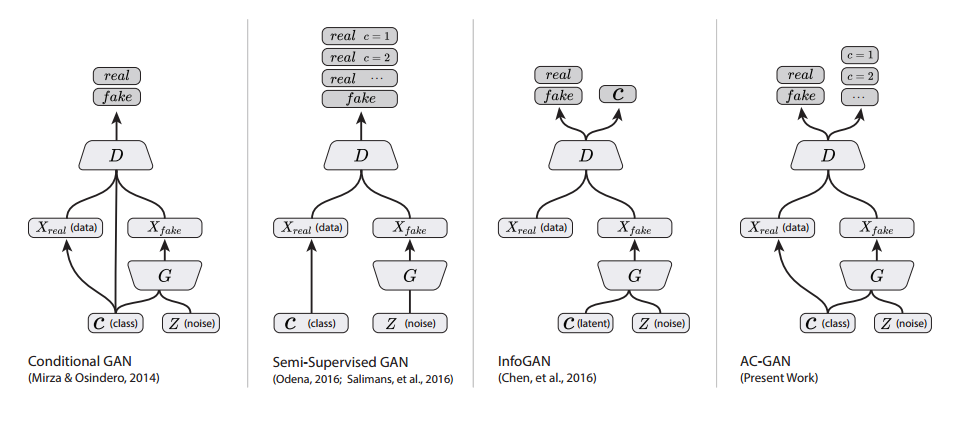
\includegraphics[width=1\textwidth]{Conditional_Architectures}
  \label{condGANs}
\end{figure}

\subsection{Generated Audio}

It was noted in the introduction that the application of generative neural network frameworks to the generation of raw audio waves has not yet received a similar intensity of research as the generation of images; despite speech synthesis being a common application that has great potential for improvement through new techniques.
The most common method of speech synthesis has been a concatentative text-to-speech method which strings together pre-recorded words or syllables in a manner that seems unnatural when compared to true speech.
\newline
\newline
A lack of suitable audio datasets for training undoubtedly retarded efforts to train effective deep neural networks for audio generation, but this is perhaps more a symptom rather than cause of the deficit of research in audio generation, given that there are two disadvantages that samples of audio have in comparison to images for deep learning.
\newline
\newline
Firstly, recordings that are meaningful to a listener need to be somewhat larger in data size than images which can equivalently be understood meaningfully.
Recordings less than a second long and with a sample rate lower than 4096 samples per second resemble little more than noise whereas the images of the \ac{MNIST} dataset are saved as only 784 pixels.
\newline
\newline
Secondly, images are quickly understood and evaluated by humans due to their instantaneous nature; the quality of an image is almost immediately discernible to an evaluator.
Images may also be printed for evaluation by readers and placed side-by-side for comparison.
In contrast, a recording needs to be listened to through a period of time to be evaluated; it is not possible to sensibly listen to multiple recordings in parallel and they cannot be printed for evaluation by readers of a journal.
\newline
\newline
The first notable application of a deep neural network to the generation of raw audio waves was DeepMind's WaveNet, this was not a \ac{GAN} but an autoregressive model \citep{DBLP:journals/corr/OordDZSVGKSK16}.
The original WaveNet could not be efficiently applied to real-time production due to the architecture requiring sequential generation of individual samples (a difficulty that \ac{GAN}s were designed to overcome) but the authors have since reported the design of an efficient Parallel WaveNet which is deployed in production for Google Assistant \citep{2017arXiv171110433V}.
\newline
\newline
There have been a small number of applications of \ac{GAN}s to raw audio since the development of WaveNet, including the \ac{SEGAN} which was created to demonstrate the application of \ac{GAN}s to the problem of denoising speech \citep{2017arXiv170309452P}; and VoiceGAN which demonstrated the application of the \ac{GAN} framework to 'style transfer' for human speech \citep{2018arXiv180206840G}.
\newline
\newline
The WaveGAN architecture which this project will explore extensions of is another recent application of the \ac{GAN} framework to raw audio; it was developed as a competitor to the WaveNet architecture and was initially reported as generating superior quality audio and having the advantage of parallel sample generation \citeauthor{2018arXiv180204208D}.
\newline
\newline
The second advantage has however been rendered void by the introduction of the more efficient Parallel WaveNet and WaveGAN has a disadvantage in comparison to WaveNet; it is currently only capable of generating audio samples of a preset length whereas WaveNet may generate audio of arbitrary length.
\citeauthor{2018arXiv180204208D} have however reported continuing work on an extension to WaveGAN that will allow for the generation of arbitrary length samples; so there is healthy competition currently in the development of generative audio.

\newpage

\section{Model Design}

Generative Adversarial Networks consist of two neural network models, a generator and discriminator, competing in a minimax game with the goal that the generator will be trained to produce new samples of data at a high standard.

\subsection{WaveGAN Model}

WaveGAN is a modified \ac{DCGAN} architecture adjused to train with 1-dimensional audio datasets instead of 2-dimensional image datasets \citep{2015arXiv151106434R}.
It follows the architectural recommendations of \citeauthor{2015arXiv151106434R}: replacing pooling layers with convolution layers; using \ac{ReLU} activation function in all generator layers other than the output; and using LeakyReLU activation function for all layers in the discriminator.

\subsubsection{Architecture}

The architecture for the WaveGAN model designed for this project was a modification of the original WaveGAN, the major difference being the reduction of the number of layers in both the generator and discriminator.
\newline
\newline
The generator had the lowest convolution layer removed as the original WaveGAN was generating samples of size 16,384; the modified version outputs layers of size 4,096.
Conversely, the discriminator had the uppermost convolution layer removed; in that case the layer was accepting input samples of size 16,384 but the modified WaveGAN accepts samples of size 4,096.
\newline
\newline
The reduction of the count of layers required an adjustment of the number of filters applied to the convolution layers at each level so that the generator and discriminator have the correct tensor dimension size at the input and output convolution layers.

\subsubsection{Generator}

The \textit{z} input to the generator is a length 100, 1-dimensional array of real numbers between -1 and 1, sampled from a uniform distribution.
This array passes through a dense layer that transforms it into a tensor with dimensions suitable for the first convolution layer; a layer with length of 16 and 256 filters.
\newline
\newline
The data then passes through a series of transposed convolution layers each with a larger length but a reduced count of filters; these layers use a kernel of size 25 and a stride distance of 4.
Each of the convolution layers is followed by a ReLU layer that retains only the positive aspect of the real numbered data.
\newline
\newline
The output layer of the generator is a tanh function which represents a hyperbolic tangent; the effect is to ensure that the data is mapped to the range -1 to 1.
The output of the tanh function is a generated raw audio waveform (Table \ref{tab:WGAN_Gen}).

\subsubsection{Discriminator}

An audio sample is passed into the discriminator as a parameter and enters the first convolution layer of length 4,096.
The data is then passed through a series of alternating layers: 1-dimensional convolution (with kernel size 25 and stride length 4), LeakyReLU, and phase shuffle.
Finally the data is reshaped then passed through a dense layer that outputs single digits (Table \ref{tab:WGAN_Dis}).

\subsubsection{Phase Shuffle}

The original WaveGAN experiment showed that audio generated by transposed convolution layers tends to produce artefacts at linear multiple frequencies of the sample rates of each convolution layer \citep{2018arXiv180204208D}.
Phase corresponds to the alignment of audio samples along the time dimension; in audio processing the phase is used in reference to the exact alignment of stereo tracks in relation to each other.
\newline
\newline
Shuffling the phase of the audio between convolution layers was shown by \citeauthor{2018arXiv180204208D} to reduce the occurrence of these artefacts in the sound.
This shuffling involves the shift of the 1-dimensional audio layer forwards or backwards by a random number of sample positions at each layer; for this project the a phase shuffle layer was placed between the convolution layers of the discriminator and the number of sample positions moved was a random number between -2 and 2, as recommended on the basis of the experimental results of the WaveGAN experiment.
\newline
\newline
This shifting of the entire data layer forwards or backwards results in some samples being moved out of the layer, and data being removed from other samples. This problem is resolved through 'reflection' where the samples that are moved out of the layer are placed back in at the opposite end, where there would now be missing samples.

\subsubsection{Adam Optimiser}

The Adam optimiser is an algorithm that is used in place of stochastic gradient descent to update network weights in a neural network.
It combines the advantages of two other variants of stochastic gradient descent, AdaGrad and RMSProp, to allow for the adaptation of parameter learning rates depending on both the mean and uncentered variance of the gradients.
\newline
\newline
Adam is generally considered the default optimisation algorithm for \ac{GAN} (perhaps influenced by the recommendations of \citeauthor{2015arXiv151106434R} in their paper introducing \ac{DCGAN}) and was chosen for the original WaveGAN model.
It is used to update both the generator and discriminator with variable learning rates depending on the selection of hyperparameters for each training run.

\subsubsection{Wasserstein Loss with Gradient Penalty}

The Wasserstein metric is a measure of the distance between two probability distributions that may be used to calculate the minimum cost of transforming a first probability distribution into a second.
This metric is colloquially known as the 'earth mover's distance' (EMD) due to the common conceit that the probability distributions are sets of piles of earth; one set being the piles of earth as they actually are, and the other set as we would like them to be, with the distance being the number of steps needed to effect the transformation from one to the other.
\newline
\newline
Loss functions based on the Wasserstein metric transform the discriminator in a \ac{GAN} from being a critic of the generator to an assistant that helps the generator estimate the distance between the real and generated distributions.
Unfortunately, these functions require a method called 'clipping' to enforce a Lipschitz constraint on the output, with the consequence that the capacity of the models and their ability to model complex functions is reduced.
\newline
\newline
The original WaveGAN used a loss function that is a modification of the Wasserstein GAN loss function but which also avoids the necessity for clipping through the introduction of a gradient penalty that ensures the Lipschitz constraint remains close to the target norm value of 1.
It has been demonstrated that the Wasserstein loss function with gradient penalty for \ac{GAN}s increases the stability of training \citep{2017arXiv170400028G}.

\subsection{Conditional WaveGAN Model}

There are a variety of methods for conditioning the inputs to \ac{GAN}s; this report has previously noted that major methods include simple concatenation, a semi-supervised architecture, the InfoGAN architecture, and the auxiliary classifier architecture.
The current project will attempt two different methods of conditioning; the first is the simple concatenation of \citeauthor{2014arXiv1411.1784M} and the second is the auxiliary classifier method devised by \citeauthor{2016arXiv161009585O}.
\newline
\newline
The concatenation method is chosen as it is the first and simplest of the methods to apply and requires very little change to the original WaveGAN architecture.
The auxiliary classifier architecture has been chosen as it was deliberately devised to include the best features of both the semi-supervised and InfoGAN architectures.

\subsubsection{Concatenation}

The concatenation method requires the introduction of labels specifying the class of each sample into both the generator and the discriminator.
The labels are passed as parameters to the neural networks and then concatenated onto the \textit{z} within the generator and the true data sample in the discriminator.
\newline
\newline
In order to concatenate this extra labelling information onto the tensors within the generator and discriminator, the labels (which are originally created as one-hot labels) are transformed into embedding layers.
An embedding layer is similar in structure to a one-hot label but is transformed so that the 'zeroes' and 'ones' do not only fill a single point within a tensor, they instead fill an entire dimension.
\newline
\newline
The embedding layer for the generator matches on multiple dimensions the size of the \textit{z} random input after it has been transformed by the initial dense layer; except that the dimension on which it will be concatenated has a length matching the number of modes of data within the dataset (Table \ref{tab:CWGAN_Gen}).
These layers that match the modes of the data are ordered to represent those modes; the first layer will match the first mode, the second layer will match the second mode, and so forth.
Each of these layers then completely fills the entire dimension with 'zeroes' or 'ones'; the layer with 'ones' representing the mode of data on which the generator should be conditioned.
\newline
\newline
The discriminator is similarly conditioned with an embedding layer which matches the dimensions of the input samples; the length of the embedding layers is 4,096 but the embedding layers are placed in separate channels and concatenated onto the true samples (Table \ref{tab:CWGAN_Dis}).
\newline
\newline
The introduction of the embedding layers also required changes to the Wasserstein-GP loss function; the discriminator call within the function was adapted to also accept the embedding layers for the true data samples.
\newline
\newline
A second simpler loss function was also tested with the concatenation method of conditioning; this second loss function calculated the loss via the mean of the sigmoid cross entropy of raw logits being provided by the discriminator (in this case the final dense layer from the baseline WaveGAN was bypassed and an extra convolutional layer was introduced to output the logits.)
\newline
\newline
A novel method of conditioning the discriminator was also tested; in this case the embedding layers were not concatenated onto the true data sample but were instead multiplied with the true data sample.
The result of this operation is to produce a new tensor that has the same dimensionality as the original embedded layer tensor but with the dimension that would be filled with 'ones' instead containing the data samples that represent the true data.
In this case the data sample is conditioned by the channel that it has been multiplied into rather than an extra layer of 'ones'.

\subsubsection{Auxiliary Classifier}

The second method to be used to introduce conditioning to WaveGAN was the \ac{ACGAN} framework developed by researchers at Google Brain.
This method was designed to take advantage of two different strategies that had been introduced in previous conditional \ac{GAN} architectures: class conditioning via concatenation and the introduction of an auxiliary decoder tasked with reconstructing class labels \citep{2016arXiv161009585O}.
\newline
\newline
The class conditioning via concatenation occurs only within the generator of the \ac{ACGAN} framework (Table \ref{tab:ACGAN_Gen}).
There is no difference in methodology here in comparison to the simpler concatenation model of conditioning; an embedding layer is passed into the generator along with each random \textit{z} array and is concatenated onto the output of the dense layer that transforms the noise into a tensor of the correct dimensionality.
\newline
\newline
The discriminator however is unlike the conditional GANs discriminator as it doesn't accept an embedding layer for concatenation conditioning and it also outputs two different probabilities (Table \ref{tab:ACGAN_Dis}).
The first probability to be output is identical to that produced by the baseline WaveGAN discriminator; a probability that the audio sample tested is either from the real dataset or is instead a sample output by the generator.
The second probability however is the probability that the sample is sampled from any of the modes of data existing within the dataset:
\newline
%
\begin{equation}
  P(S|X), P(C|X) = D(X)
\end{equation}
%
\newline
The loss function for the \ac{ACGAN} has two components; firstly a calculation of the loss via the mean of the sigmoid cross entropy of the logits, identical to the loss function that has previously been described as having been tested with the concatenation method of conditioning; and secondly, the calculation of the mean of the softmax cross entropy of the categorical logits and one-hot arrays representing the classes defined for the real dataset and generated samples.
The sum of both of these component losses for the generator and discriminator are then output as the final loss.

\subsection{Hyperparameter Search}

A key difficulty in training \ac{GAN}s is finding a set of hyperparameter values that allow the networks to converge and successfully train the generator to produce interesting samples.
Much research into the properties of \ac{GAN}s is driven by the desire to understand how the hyperparameters influence the training and how they may be selected via automatic methods.
\newline
\newline
Initial testing of the baseline WaveGAN framework developed for this project showed that the hyperparameters used for the original WaveGAN model were not transferable to the downsized model, despite being trained on the same data and differing only in the number of layers in the generator and discriminator.
These tests showed early divergence within the loss function with the discriminator loss falling rapidly to negative infinity and the generator loss increasing rapidly to positive infinity; suggestive of the discriminator overpowering the generator.
\newline
\newline
A series of tests of the various hyperparameters were therefore run so as to discover the effect each had on the likelihood of the networks diverging and no longer being able to learn.
The results of a number of these tests are produced as tables in the appendices.
\newline
\newline
Testing proceeded on three different versions of the models; the baseline WGAN and two versions of the conditional WGAN model each with slightly different implementations of the conditional Wasserstein-GP loss.
These models were also reduced versions of those that would eventually be used for the final experiments; they tested and generated audio samples of size 1,024, a convolution layer smaller than the final networks.
\newline
\newline
The parameters initially tested were the batch size, the Adam optimiser learning rate, the Wasserstein-GP loss lambda variable, and the relative proportion of discriminator to generator updates per iteration of the model.
The parameters were tested over a series of values for five thousand iterations; early stopping was introduced for the models when either the absolute discriminator or generator loss value passed 100 (chosen based on previous tests showing this value was only ever passed when the networks started to diverge).
\newline
\newline
Each model was tested with every chosen value for each parameter ten times and the number of iterations reached before divergence (rounded down to the nearest thousand) were recorded, unless the number of iterations reached 5,000, at which point the test was complete. 
During the testing of values for each hyperparameter, all other hyperparameter values were maintained at the values which were reported as successful for the original WaveGAN model.
\newline
\newline
The tests were adapted throughout the process as some parameter values were quickly revealed to be unusable and then dropped from further tests.
Early results also showed that one of the implementations of the conditional Wasserstein-GP function was superior to the other and from that point onwards the inferior implementation was dropped from testing.
A small number of tests were also run on the larger network models that dealt with audio sample rates of 4,096 samples per second; these confirmed that the trends in the values were relatively consistent across the models of different sizes.
\newline
\newline
Results showed that the values chosen for each of the tested hyperparameters had varying effects on whether and how early the generator and discriminator losses were likely to diverge; although it was also clear that there was a large degree of randomness determining how quickly any particular test would result in divergence.
\newline
\newline
Batch size had a clear effect on the likelihood of a model diverging but it was not initially clear whether this was evidence that smaller batch sizes resulted in more stable training, or whether this was the result of a slow down in the overall training of the models, with the training of each epoch simply taking more iterations.
\newline
\newline
The Adam optimiser learning rate had a clear effect on whether a model was likely to diverge early; the initial value used for the original WaveGAN model (1e-4) was found to be too high for the tested models as they all diverged very early.
The tests showed that lower values (from 1e-5) were far more likely to avoid early stopping.
\newline
\newline
The lambda variable within the Wasserstein-GP loss function also displayed a noticeable effect on the number of iterations passed before the divergence of the loss function.
Higher lambda values tended to prolong the training and avoid early stopping whereas any lambda value less than 10 with the original WaveGAN model hyperparameters was very likely to diverge early.
\newline
\newline
The proportion of discriminator to generator updates was tested with the number of discriminator updates either equal to or larger than the number of generator updates; this choice was made with consideration that the original WaveGAN model used a rate of five discriminator updates to each generator update.
The tests showed that with even an equal number of iterations the models only avoided diverging before 5,000 iterations approximately half of the time; suggesting that the discriminator was relatively more powerful than the generator.
\newline
\newline
Tests of larger proportions of generator to discriminator updates were not completed at this stage as consideration was first given to other methods that might decrease the power of the discriminator, such as the addition of Gaussian noise to the discriminator input layer and the use of soft and noisy labels in the loss functions.
\newline
\newline
The hyperparameter search was extremely useful as it revealed the tendencies of each parameter to effect the likelihood of divergence.
Unfortunately it did not however reveal any parameter values as having a dominant and stabilising effect on the training and further testing was required during the experimentation stage of the project.

\newpage

\section{Data}

The architecture and functions of a neural network model are to some degree determined by the dataset chosen for training; in this case a dataset has already been created for experiments with digital audio, the \textit{Speech Commands Dataset} \citep{speechcommands} but we will see how it has been adapted for \ac{GAN} experiments.

\subsection{Characteristics of Digital Audio}

The major characteristic of audio data is that it is 1-dimensional and is understood only through passage in the time dimension.
Audio data may be mono or stereo, or may have even more channels than stereo (such as audio used with surround sound systems) but this experiment focuses on mono audio only with 1 channel only.
\newline
\newline
Digital audio separates the single time dimension into points of measurement that are referred to as samples; these samples each describe a point on a complex sound wave which is the result of multiple intermixed frequencies.
For digital audio to be heard as sound, the digital stream of these measurements must be converted into analogue at the point where sound is introduced into the environment, such as via speakers, headphones or audio monitors.

\subsubsection{Comparison with Images}

This report has already noted that audio has disadvantages compared to images when being considered as a dataset for \ac{GAN} training but these disadvantages are worth further consideration as they have some consequences for the training process.
\newline
\newline
Images are static and can be evaluated almost instantaneously; they have an immediacy that audio recordings do not.
A human evaluator only needs to look at an image and can almost immediately judge whether it is a realistic representation of a figure or not; but to evaluate the quality of an audio recording the human evaluator must listen for a set period of time.
\newline
\newline
A consequence of audio requiring a set period of listening time is that it is more difficult to compare audio recordings to each other than it is to compare images.
When comparing images the evaluator may have both images available in their vision and may quickly move their focus between them; when comparing audio however they must first fully listen to one sample before they may then consider the other, and must retain in memory the segments they wish to compare.
\newline
\newline
This time taken to switch between audio samples and the need to hold the evaluation of one sample in mind while listening to another makes comparison difficult.
Long samples increase the difficulty of retaining in memory the section of the sample the evaluator wishes to compare; slicing the samples into small sections may help but introduces the difficulty of trying to understand slices of audio outside of the context of the recording.
\newline
\newline
There is also a difference in the size (in terms of data) of an image that can be comprehended by a human evaluator and the size of an audio sample that can be comprehended; very small images may be easily understood, especially if they contain symbolic representations such as letters or numerals.
Small audio files are however less easily understood by an evaluator; they cannot be resized as images can without fundamentally changing the nature of the sound being represented.
\newline
\newline
For example, the shortening of a sound may have two consequences: if done naively the pitch of the audio recording will increase until it bears little resemblance to the original recording; at moderate levels this produces a 'chipmunk' effect but beyond that the sound becomes unrecognisable; however, if the recording is shortened with an algorithm that maintains the original pitch, then the sound still becomes unrecognisable because it passes at a speed beyond comprehension.
\newline
\newline
Another method of reducing the size of an audio sample is to lower the sample rate; this may be effective to a certain degree as audio often contains frequencies which are not essential for human comprehension of the sounds.
However, this method may reduce the size of the recording in terms of the amount of data used for storage but it doesn't reduce the time required for a human listener to evaluate it.

\subsection{Graphical Representation of Audio}

The difficulty in evaluating audio samples during the training process required the introduction of visual feedback to facilitate monitoring, and especially to assist in deciding whether training should continue or be stopped and restarted.
Graphs showing the wave and spectogram of the real and generated audio samples were therefore output to the tensorboard monitoring dashboard.
\newline
\newline
The first plot type shows the wave of the audio files with the time dimension displayed on the \textit{x} axis and amplitude of the audio shown on the \textit{y} axis.
The peaks and troughs in the graph correspond to the changes in the amplitude of the frequencies over the time period of the audio recording; these plots can show how the shape of the generated samples changes from random noise to something similar to a true recording.
\newline
\begin{figure}[ht]
  \caption{Example of an audio waveform plot}
  \centering
  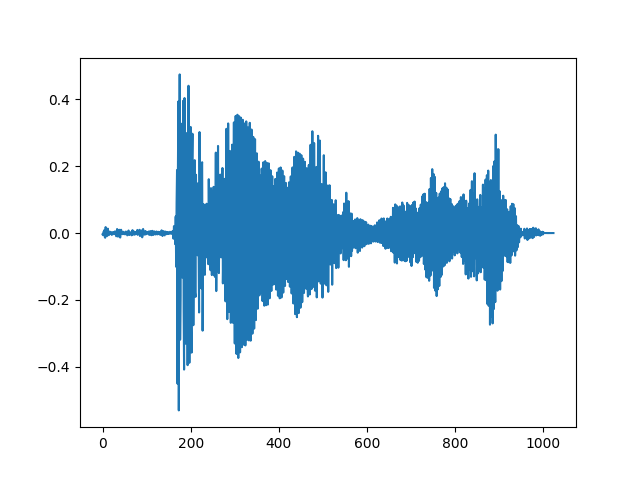
\includegraphics[width=0.75\textwidth]{AudioWave}
\end{figure}
\newline
The second plot type is a spectogram which shows how the frequencies of the audio samples vary over the time dimension: the \textit{x} axis displays the time dimension separated into bins that group frequencies over a period of time together; the \textit{y} axis represents the pitch of the frequencies, with lower frequencies near the bottom and higher frequencies near the top.
The spectogram also has a third dimension; the colour represents the amplitude and intensity of the frequencies.
\newline
\newline
The spectogram was useful to monitor how the generated samples were transforming over the epochs of training; the vertical distribution of the frequencies was particularly revealing as it showed whether or not actual frequencies within the audio rather than amplitude only were being learned by the generator.
\newline
\begin{figure}[ht]
  \caption{Example of a spectogram}
  \centering
  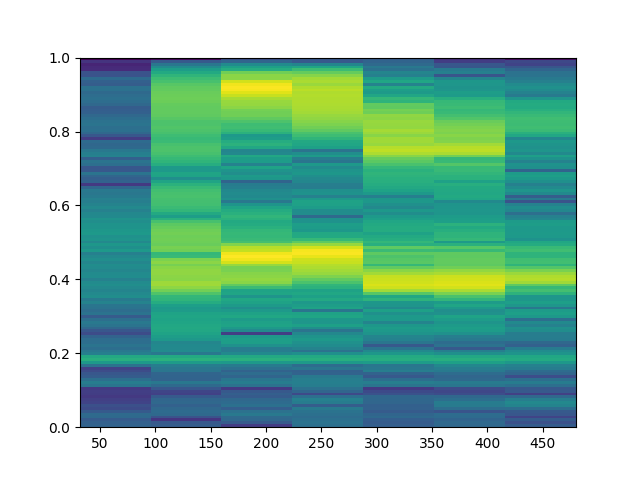
\includegraphics[width=0.75\textwidth]{AudioSpec}
\end{figure}

\subsection{Sample Rates}

The sample rate of a recording defines the count of samples that are used per second to represent sounds; higher sample rates require more data but allow higher frequencies to be captured; lower sample rates however result in smaller file sizes and lower training times.
\newline
\newline
Recordings within the \textit{Speech Commands Dataset} are approximately one second long with a sample rate of 16,000 hertz (Hz), or cycles per second.
The most recognisable features of human speech lie in the range from 30 Hz to 5,000 Hz so there is an element of redundancy in the \textit{Speech Commands Dataset}; the higher sample rate recordings sound more natural but lower sample rate audio is still recognisable as speech.
\newline
\newline
Reduction of the sample rate of audio is called 'downsampling'; this operation allows the higher sample rate recording to be reduced in size with a consequent reduction in the number of frequencies represented.
Downsampling was used for this project to reduce the computational requirements for training; the subjective quality of the downsampled audio however was still suitable for evaluation of spoken words.

\subsection{Dataset Selection}

The \ac{SC09} dataset is a subset of the \textit{Speech Commands Dataset} which includes only the ten spoken words for the numbers zero through nine; each word being represented by approximately 2,370 recordings.
This dataset contains recordings from a wide variety of alignments, spoken by a wide range of speakers, and recorded under a wide range of conditions \citep{2018arXiv180204208D}.
\newline
\newline
This dataset was used for the training of the original WaveGAN model but results in long training times; given that a minimum of two different words are required for the demonstration of conditioning, it was decided that a subset of \ac{SC09} would be used for the experiments within this project.

\subsubsection{Speech Commands Binary Dataset}

A new \textit{Speech Commands Binary Dataset} containing only the spoken words for numbers 'zero' and 'one' was therefore selected for the project.
This dataset has words of different syllable counts, with no shared syllables, and the words are easily distinguishable; the dataset also has consistency with the subject matter by representing the numbers used for digital computation.
\newline
\newline
The training set is derived from the training sets recommended for the \textit{Speech Commands Dataset} and there are 1,850 utterances of each word.
A single epoch passing through the sets of recordings for both spoken words therefore requires iteration through 3,700 samples.

\subsection{Data Manipulation}

A tool named 'Downsample.py' was written in Python to assist in the downsampling of the audio files to be used in these experiments.
It is capable of downsampling to various different sample rates and allows a listed collection of the folders (hence words) to be resampled at any time; this allows for the saving of space as it ensures only the necessary files are saved.
\newline
\newline
A function was added to check that the each resampled file originally had the expected sample rate of 16,384 samples per second so that resampling would be as clean as possible; if the sample rate is higher than expected the excess samples are trimmed off the end; if the sample rate is lower than expected then zero-valued samples are added to the end to ensure the final length of the resampled recording is one-second.

\newpage

\section{Experiments}

Experiments reported in the WaveGAN paper showed that the model converges within 700 epochs on a wide variety of datasets including spoken words, bird vocalizations, and drum and piano recordings \citep{2018arXiv180204208D}.
Given that these datasets were more complex than the \textit{Speech Commands Binary Dataset}, particularly with more modes of data in the \ac{SC09} dataset, the experiments for this project were run for approximately 700 epochs then stopped for comparison.

\subsection{WaveGAN}

Early testing and the hyperparameter search already showed that the baseline WaveGAN would fail to converge when trained using the hyperparamters reported as successfully used in the original WaveGAN experiment.
Training was therefore preceded by further tests on variations in the values of the hyperparameters to find a set that would allow for convergence.
\newline
\newline
Variations in the values for the batch size, learning rate and the ratio of discriminator to generator updates were all found to stabilize training, but only at relatively extreme values.
For example, the original WaveGAN model was capable of converging with a batch size of 64, a learning rate of 1e-4 and a discriminator to generator update ratio of 5 to 1; one of the few hyperparameter settings capable of converging with the baseline WaveGAN used for these experiments was a batch size of 8, a learning rate of 1e-5 and a discriminator to generator update ratio of 1 to 1.
\newline
\newline
Further experimentation showed that the ratio of discriminator to generator updates was key to the stabilization of the training for the baseline WaveGAN; despite recommendations that Wasserstein-GP loss be used with a discriminator to generator update ratio of 5 to 1, only the reverse ratio of 5 generator updates to each discriminator update was capable of avoiding early divergence with the recommended batch size of 64 and learning rate of 1e-4.
\newline
\newline
The discrepancy between the values that result in convergence for the original WaveGAN and the baseline WaveGAN used in this experiment needs further investigation; the discriminator is far more powerful in the downsized model compared to the original; ten times more powerful given that the ratio of updates changes from 5 to 1 with the original model to 1 to 5 with this modified model.
\newline
%
\begin{figure}[ht]%
  \caption{The discriminator loss for WGAN}
  \centering
  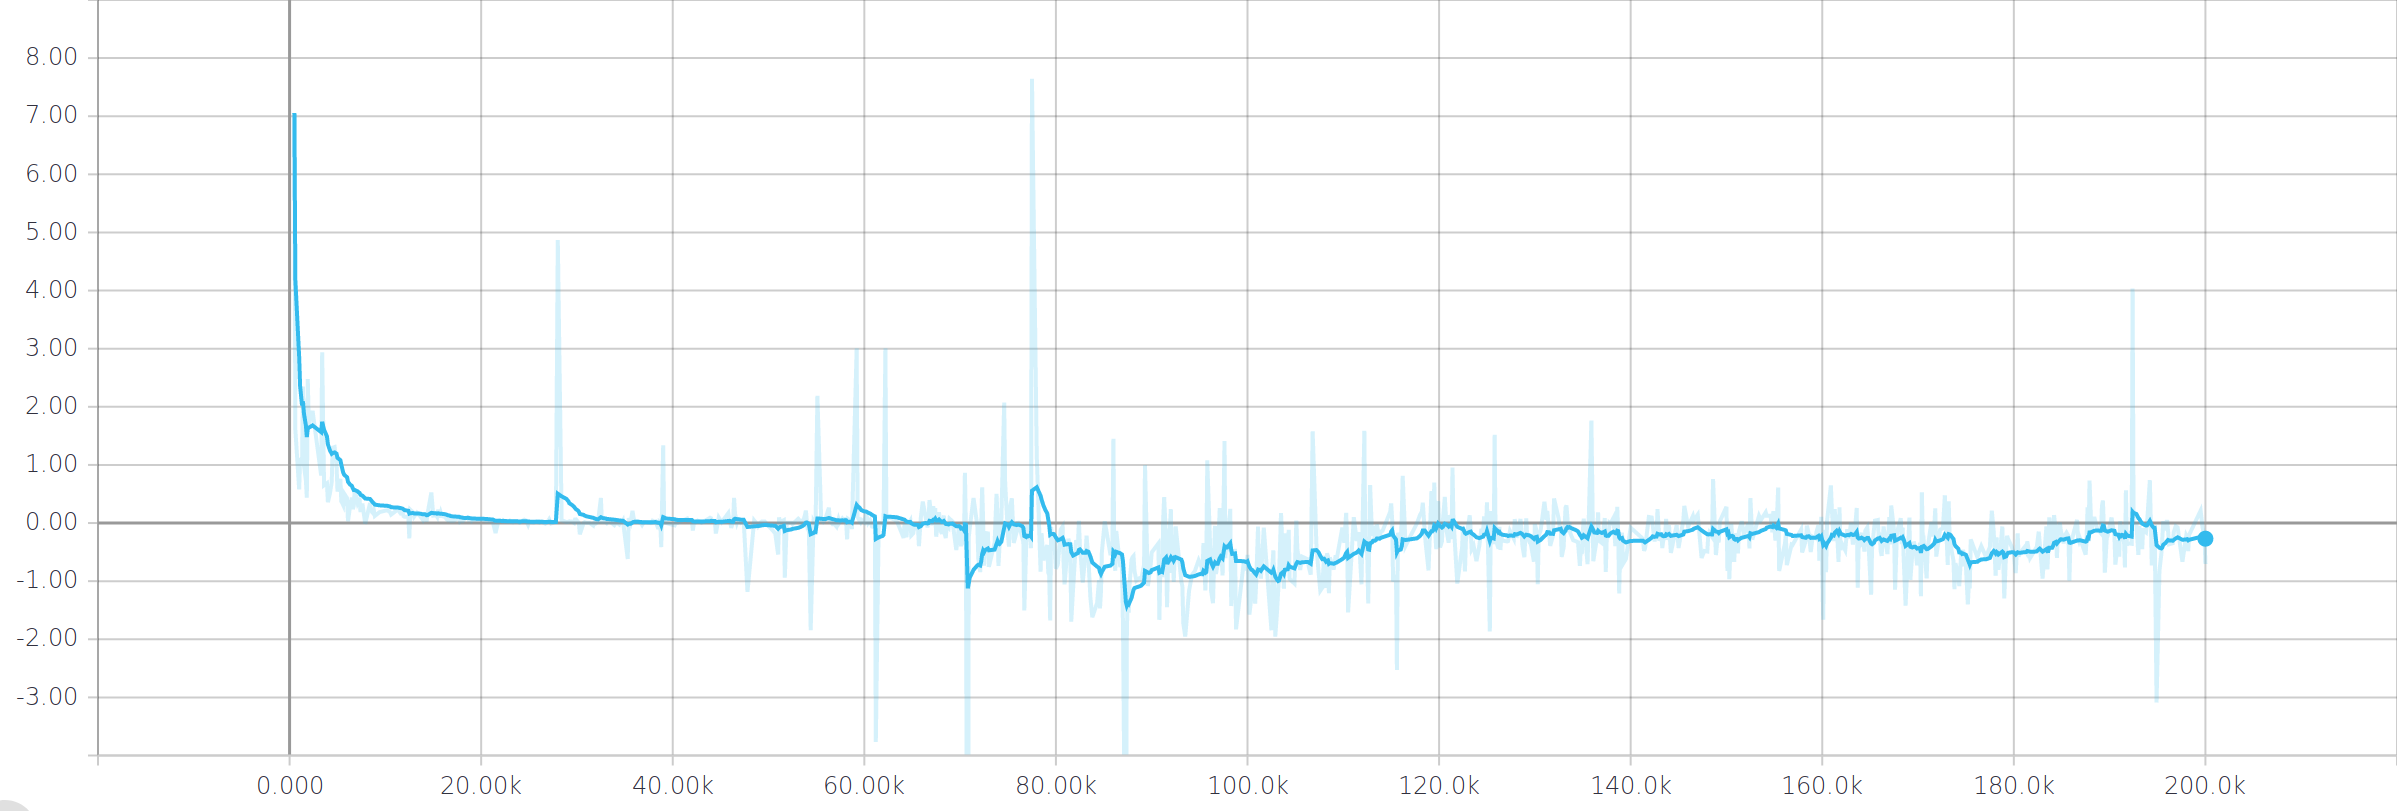
\includegraphics[width=1\textwidth, clip]{WGAN-Dis-Loss}
  \label{fig:WGAN-Dis-Loss}%
\end{figure}
%
\newline
The architecture was checked multiple times for errors that might be causing the discriminator to be overpowered but the implementation appears sound.
Since the model was ultimately capable of generating samples that were distinguishable as words, further investigation on the effect of the number of layers \textit{and the number of filters available for the transposed convolution} is a possible direction of research that might reveal the cause of this imbalance of power between the discriminator and generator.
\newline
\newline
Within the limitations of the experiment, training of approximately 700 epochs, the baseline WaveGAN was not generating high quality audio samples although they were distinguishable as spoken words.
The samples were very noisy with buzzing sounds that suggest the generator had not been able to capture the more complex interactions between the frequencies that constitute a sound.
\newline
\newline
Visual examination of the plots of the audio waves show that the generator was able to capture the shape of the amplitude of the sounds, relating to the change of the volume of the audio over the period of the sound.
These changes in amplitude were shown to be generated very early in the training and seem straightforward for the generator to learn.
The wave plots also show that mode collapse has not occurred and that the generator was capable of creating a variety of different sounds (Figure \ref{fig:WGAN-Waves}).
\newline
%
\begin{figure}[ht]%
    \centering
    \subfloat[Generated]{{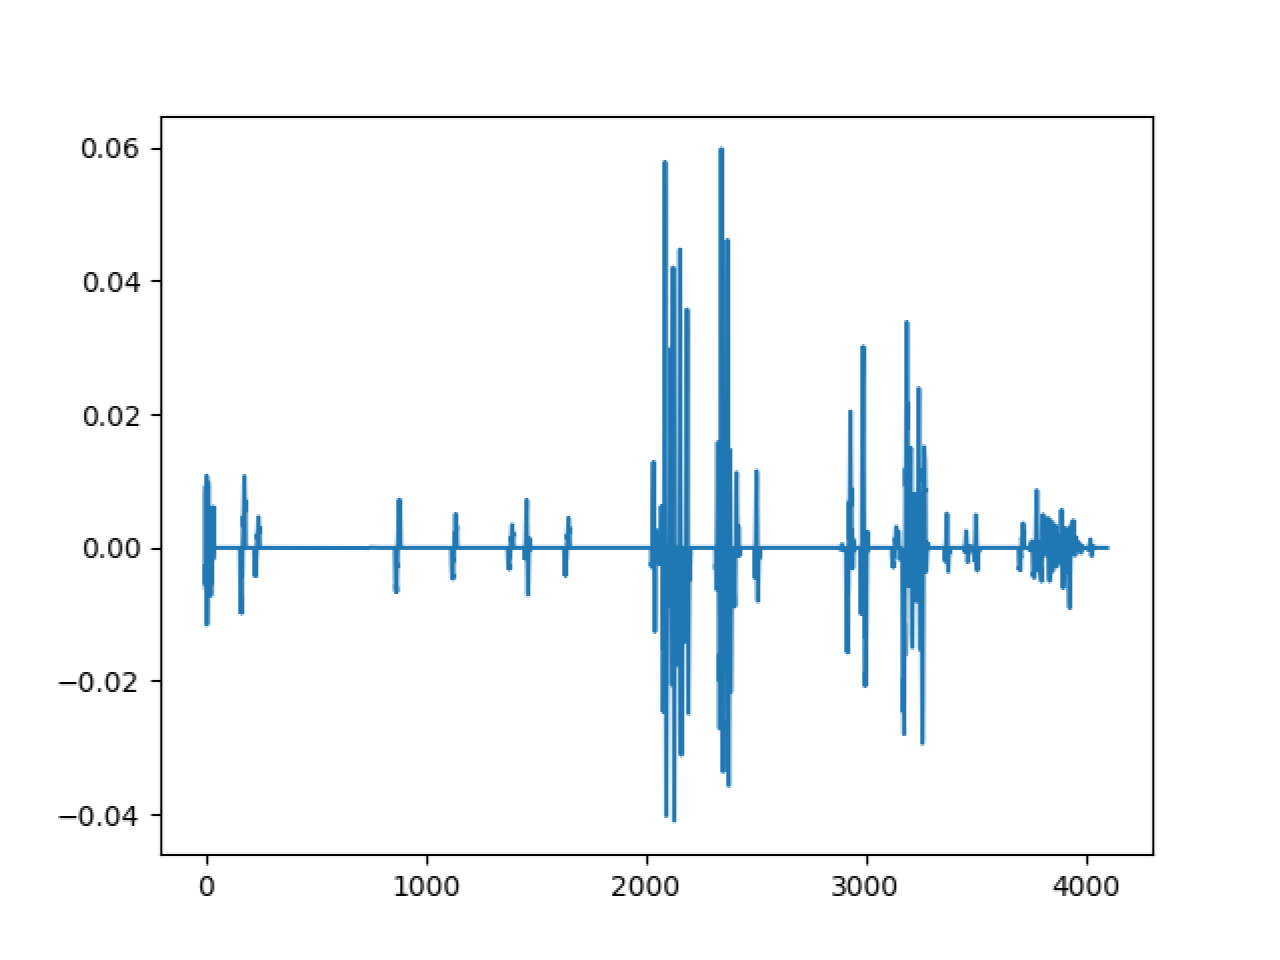
\includegraphics[width=5cm]{WGAN-Gen-Wave-1} }}%
    \qquad
    \subfloat[Generated]{{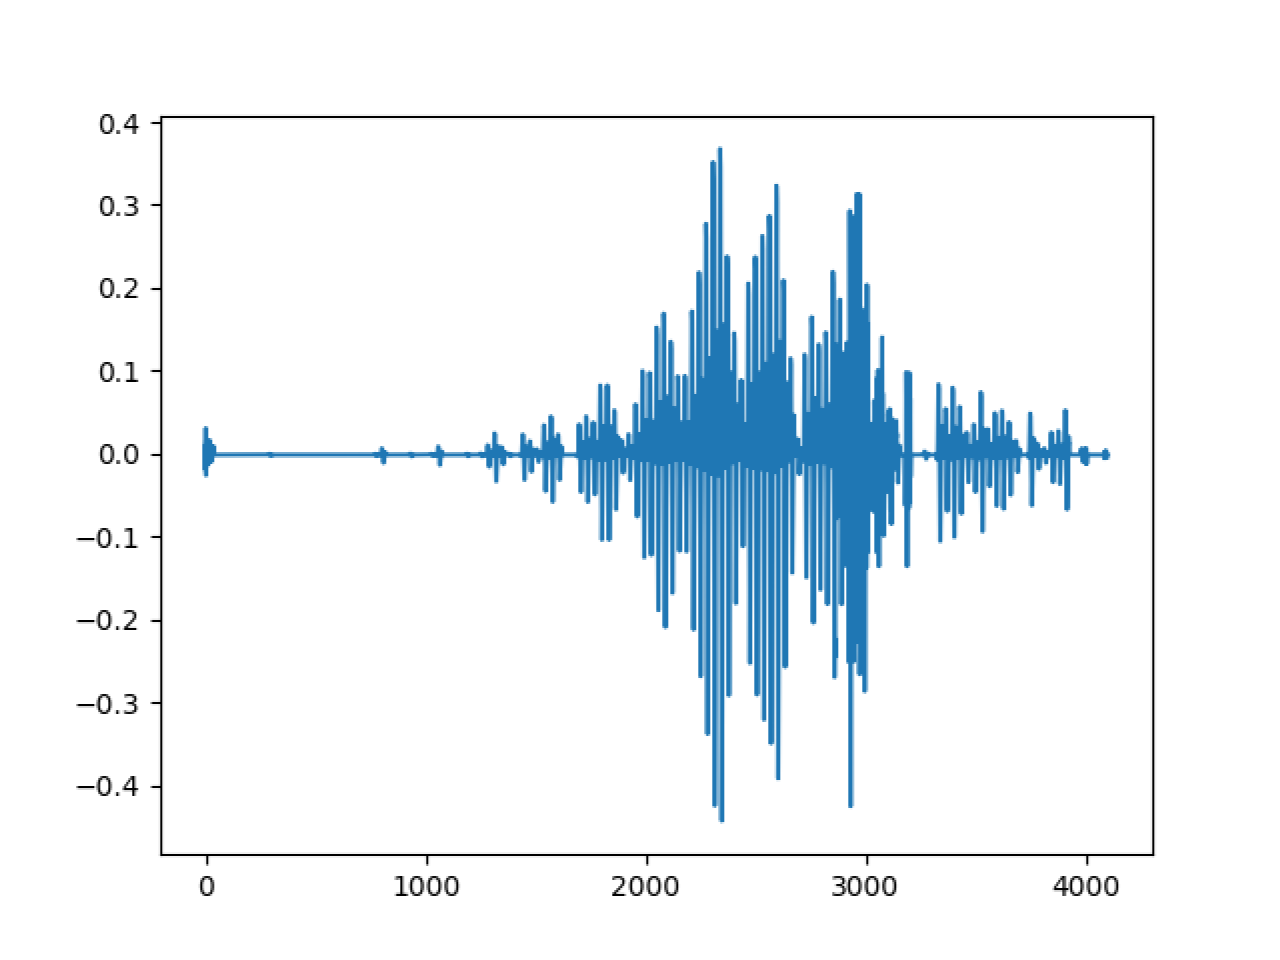
\includegraphics[width=5cm]{WGAN-Gen-Wave-2} }}%
    \qquad
    \subfloat[Real]{{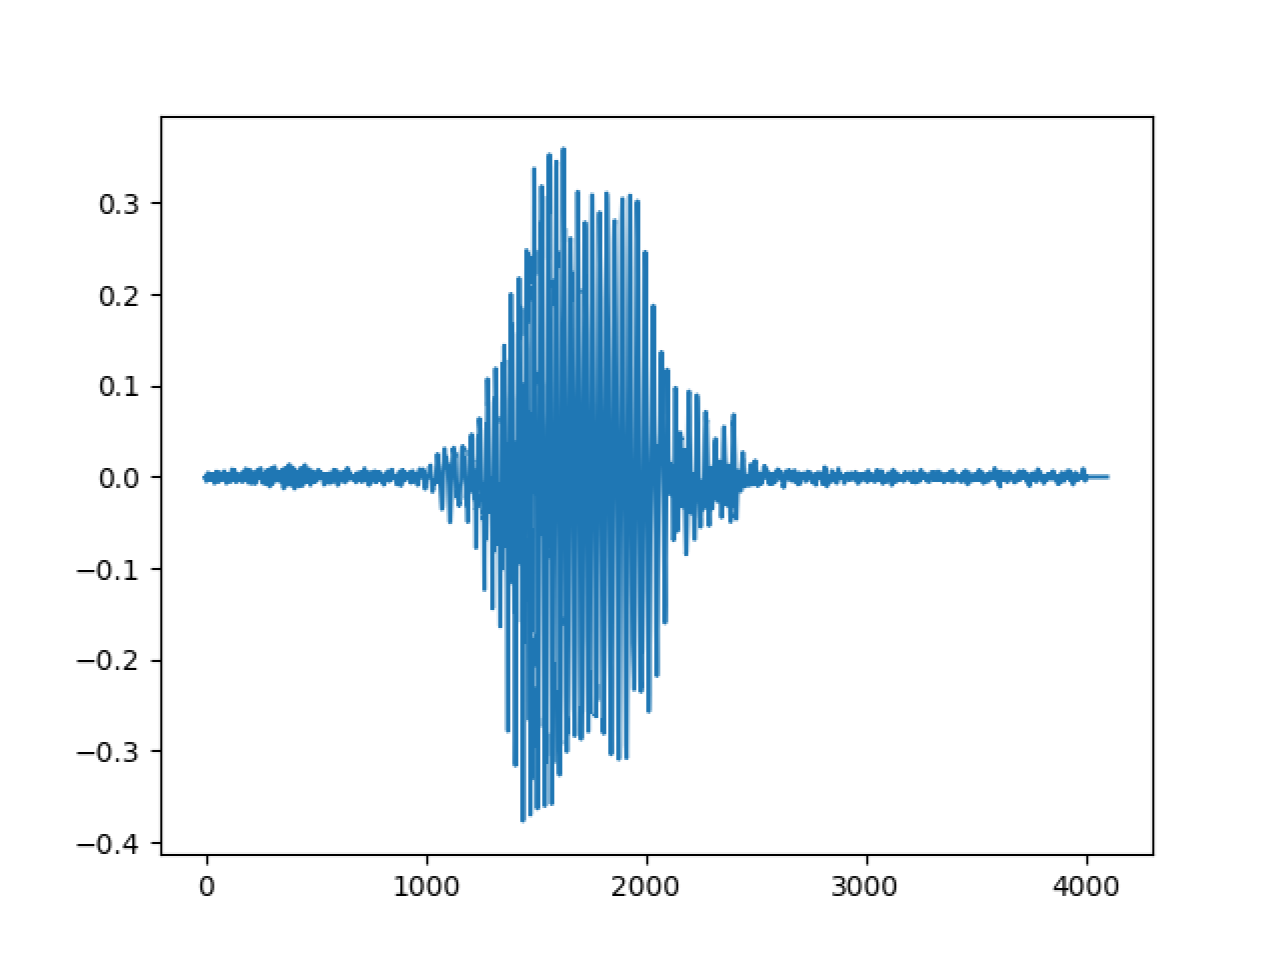
\includegraphics[width=5cm]{WGAN-Real-Wave-1} }}%
    \qquad
    \subfloat[Real]{{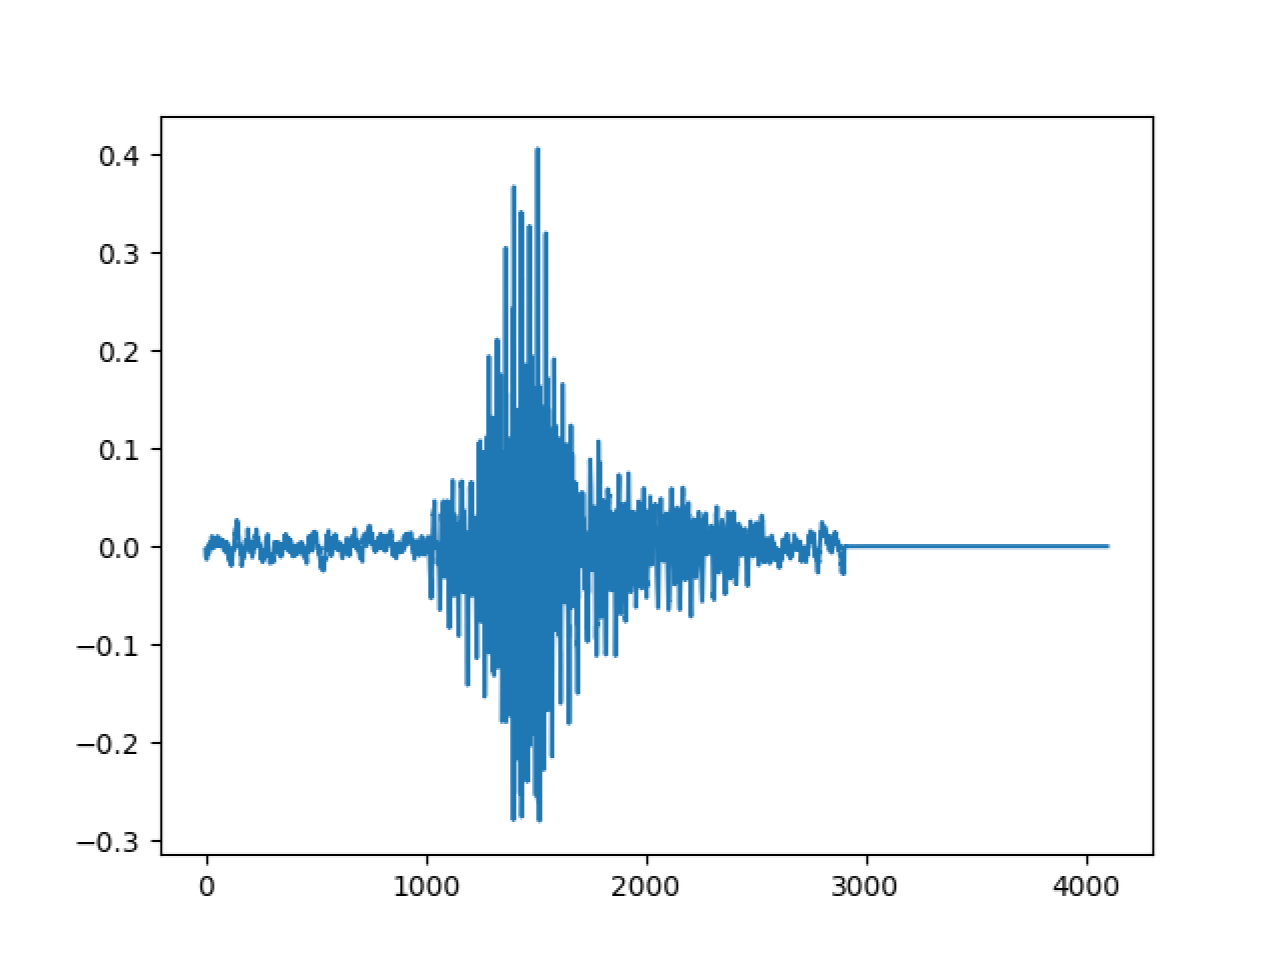
\includegraphics[width=5cm]{WGAN-Real-Wave-2} }}%
    \caption{Wave plots of WGAN generated and real samples}%
    \label{fig:WGAN-Waves}%
\end{figure}
%
\newline
The spectogram plots also show that the baseline WaveGAN is capable of generating a varied set of samples and has avoided mode collapse.
Horizontal lines of high intensity also divide the plots vertically; this shows that the model has started to capture the frequencies of the sound, but unlike the true audio samples, the lines are straight rather than curved.
Again, this suggests that high level interactions between the frequencies are not being learned (Figure \ref{fig:WGAN-Specs}).
%
\newline
\begin{figure}[ht]%
    \centering
    \subfloat[Generated]{{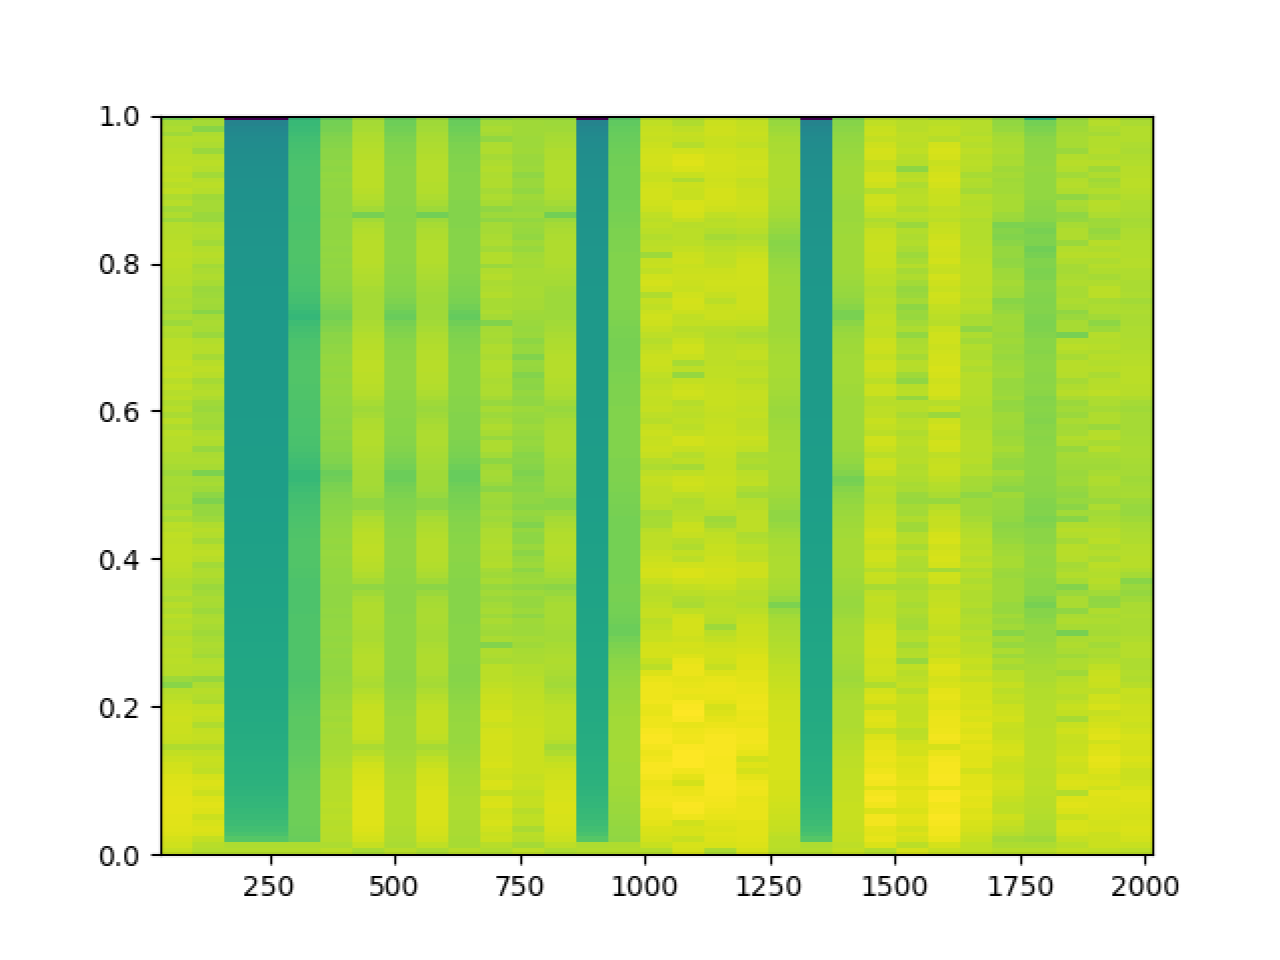
\includegraphics[width=5cm]{WGAN-Gen_Spec1} }}%
    \qquad
    \subfloat[Generated]{{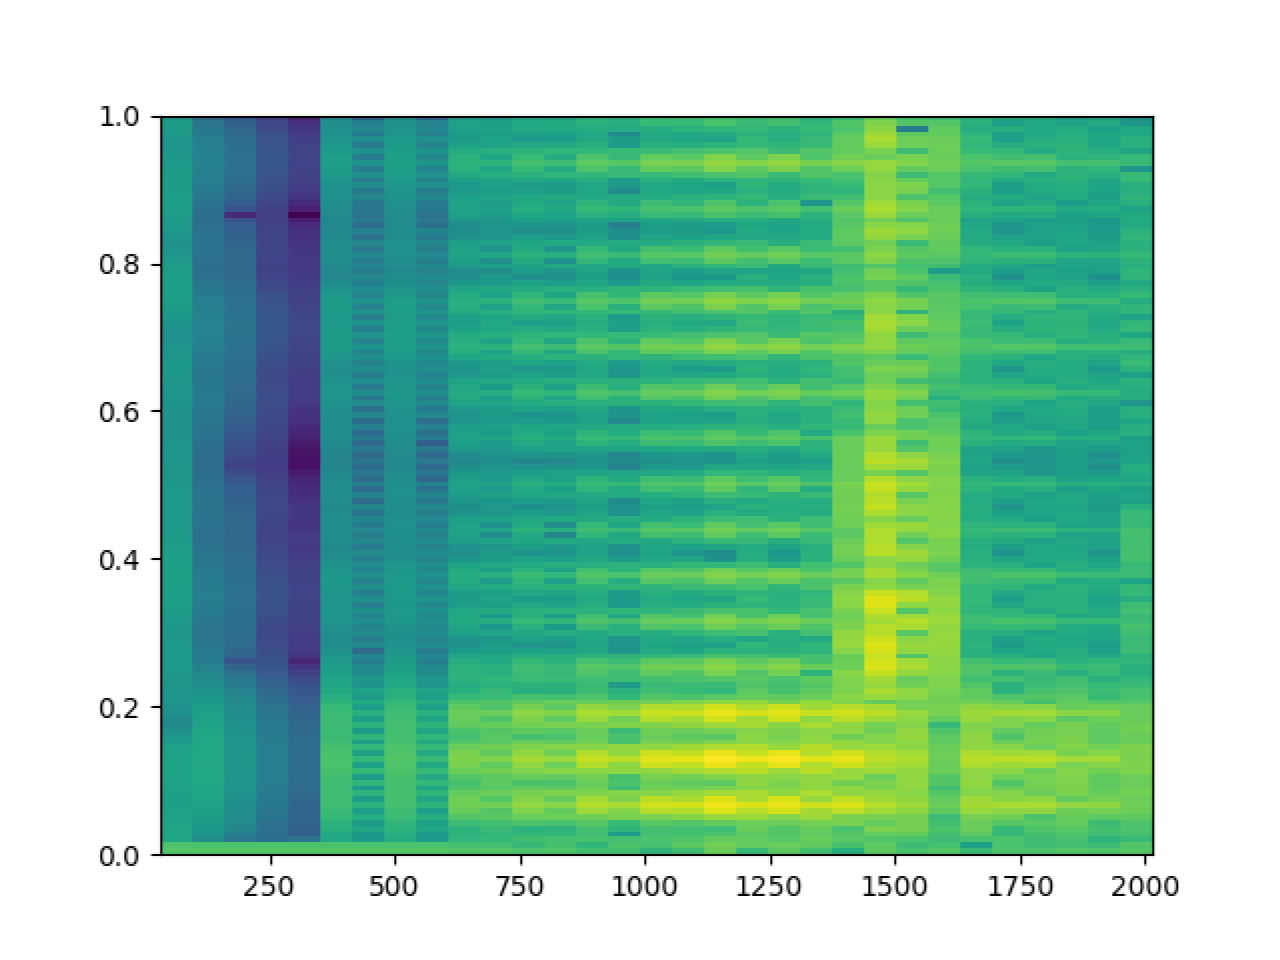
\includegraphics[width=5cm]{WGAN-Gen_Spec2} }}%
    \qquad
    \subfloat[Real]{{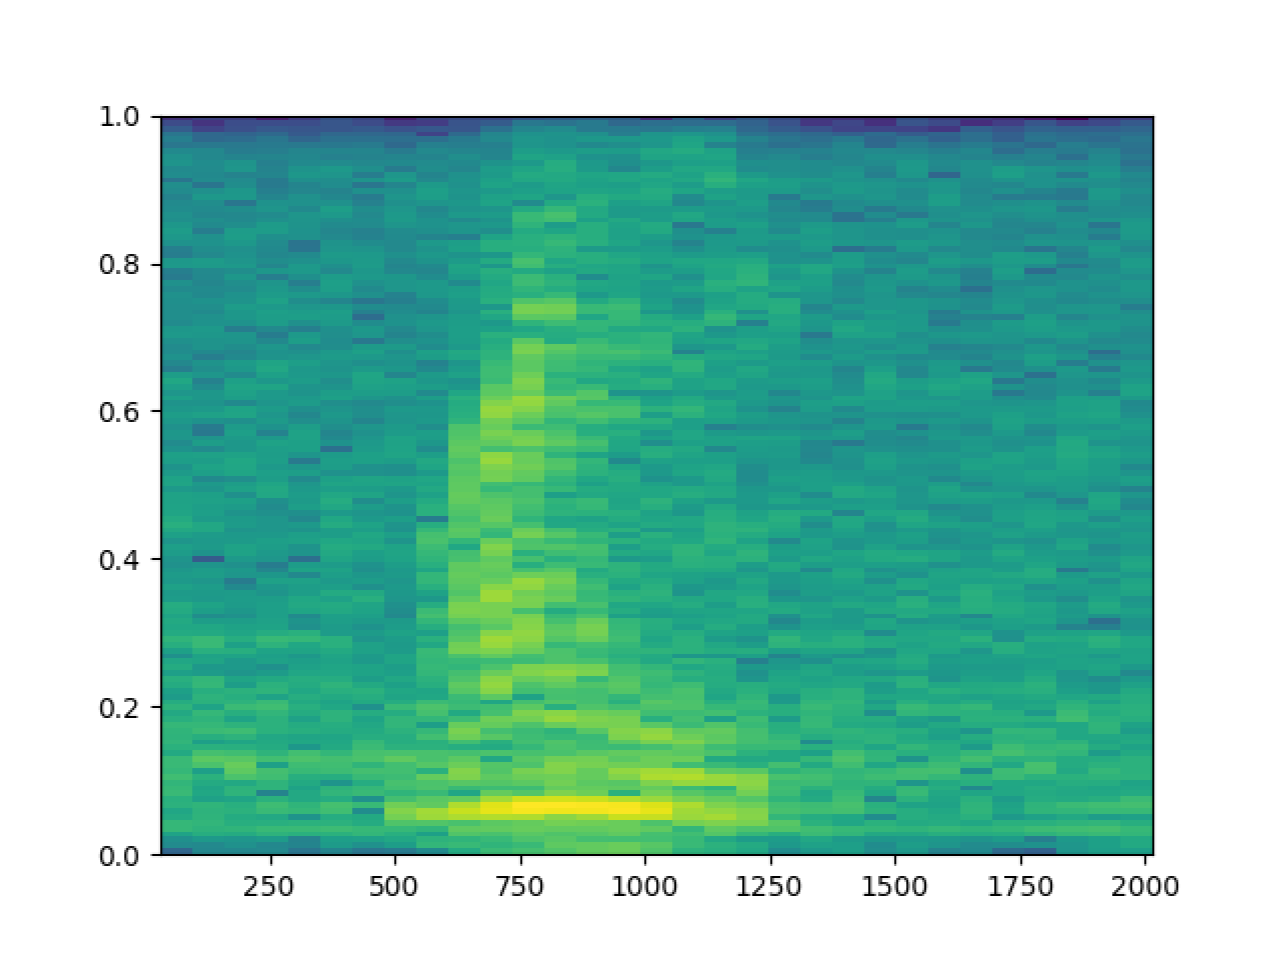
\includegraphics[width=5cm]{WGAN-Real_Spec1} }}%
    \qquad
    \subfloat[Real]{{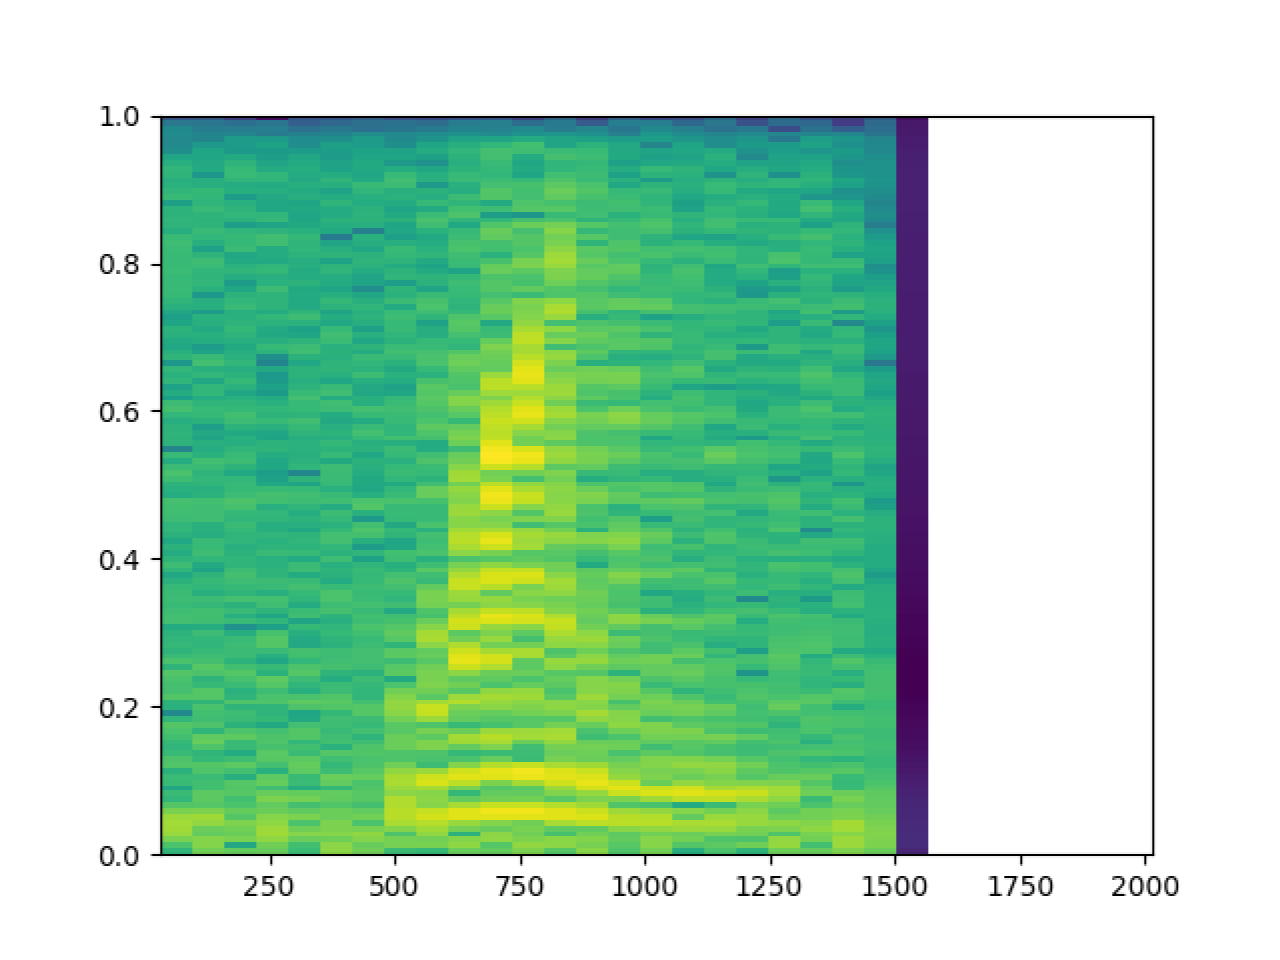
\includegraphics[width=5cm]{WGAN-Real_Spec2} }}%
    \caption{Spectograms of WGAN generated and real samples}%
    \label{fig:WGAN-Specs}%
\end{figure}
%
\newline
A review of the spectogram plots suggest that the discriminator and generator were repeating the same learning process in a cycle and the generator was unable to ultimately capture the more complex movement of frequencies over time.
Still, the baseline WaveGAN shows that it is capable of converging slowly; further training or adjusted hyperparameters that favour the generator should result in a model that generates acceptable samples.
\newline
%
\begin{figure}[ht]%
  \caption{The generator loss for WGAN}
  \centering
  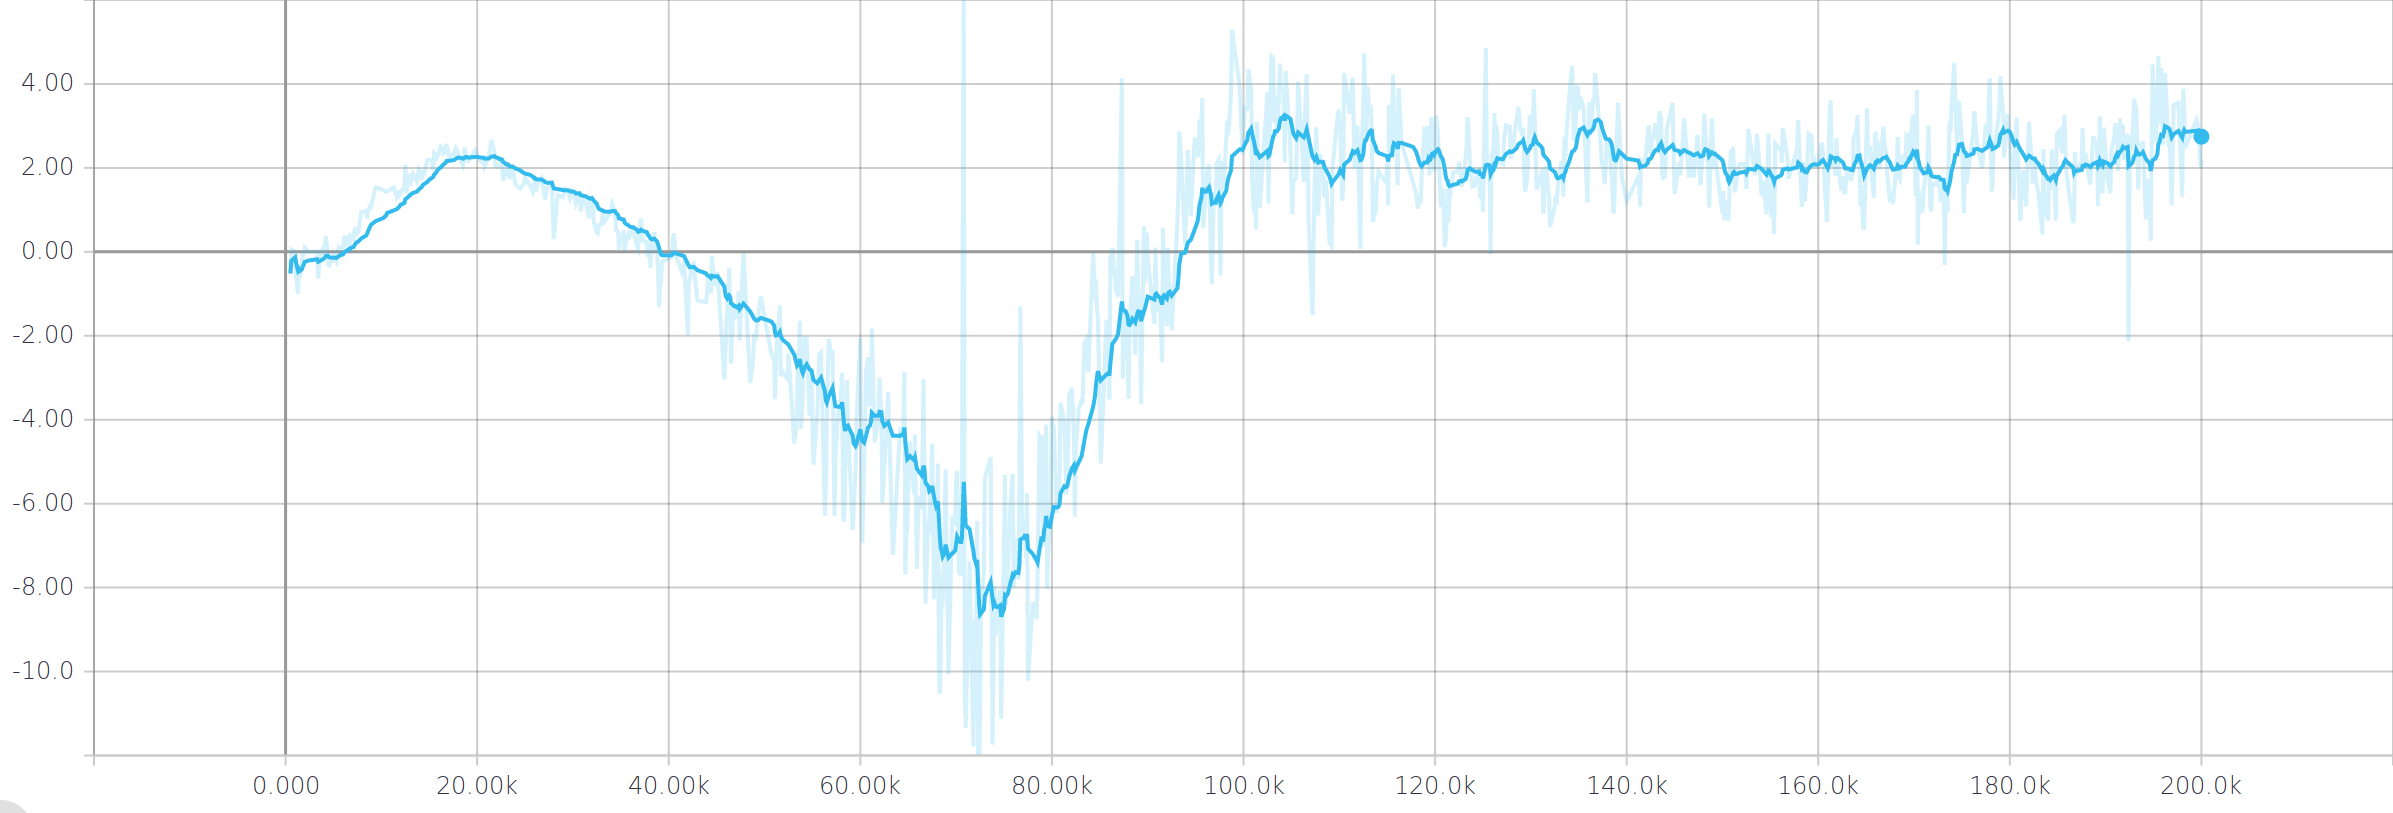
\includegraphics[width=1\textwidth, clip]{WGAN-Gen-Loss}
  \label{fig:WGAN-Gen-Loss}%
\end{figure}

\subsection{Conditional WaveGAN with Concatenation}

This methodology was unable to train the WaveGAN model successfully; the discriminator loss consistently dropped to zero within a very few epochs.
Even when the ratio of generator to discriminator updates was increased to relatively extreme values such as 8 or even 16 the generator was still unable to counteract the early drop of the discriminator loss to zero.
\newline
\newline
Using the tensor channels as signifiers of the label for each sample had a similar result as the concatenation of labels; the discriminator would still consistently drop to zero within very few epochs.
However, the removal of the embedding layer of 'ones' did seem to enable the training to take place more quickly even though it would also ultimately fail; monitoring the wave plots during training showed that the samples would arrive at a sensible shape more quickly than with the simple concatenation method.
\newline
\newline
Two different loss functions were tested with this concatenation method; the first was the conditional Wasserstein-GP loss and the second was a simpler loss calculating from the mean of the sigmoid cross entropy of the logits; neither resulted in an advantage.
The introduction of noise to samples entering the discriminator before they were passed to the first convolution layer also had no effect on the tendency of the discriminator to rapidly overpower the generator.
\newline
\newline
The concatenation method of conditioning the output of the WaveGAN model developed for this project was ultimately a total failure.
Even testing with high ratios of generator to discriminator updates, and with the ratio of generator updates increasing each time the discriminator loss dropped below set values, even to extreme values such as 60, the discriminator loss would still drop to zero within a very epochs.

\subsection{Conditional WaveGAN with Auxiliary Classifier}

The \ac{ACGAN} method was more stable than the concatenation method of conditioning but was also ultimately unable to produce high quality samples within the constraints of the experiment.
It does show some promise however and unlike the concatenation method there may be some advantage gained from training further epochs or further refining the hyperparameter choices.
\newline
%
\begin{figure}[ht]%
  \caption{The generator loss for ACGAN}
  \centering
  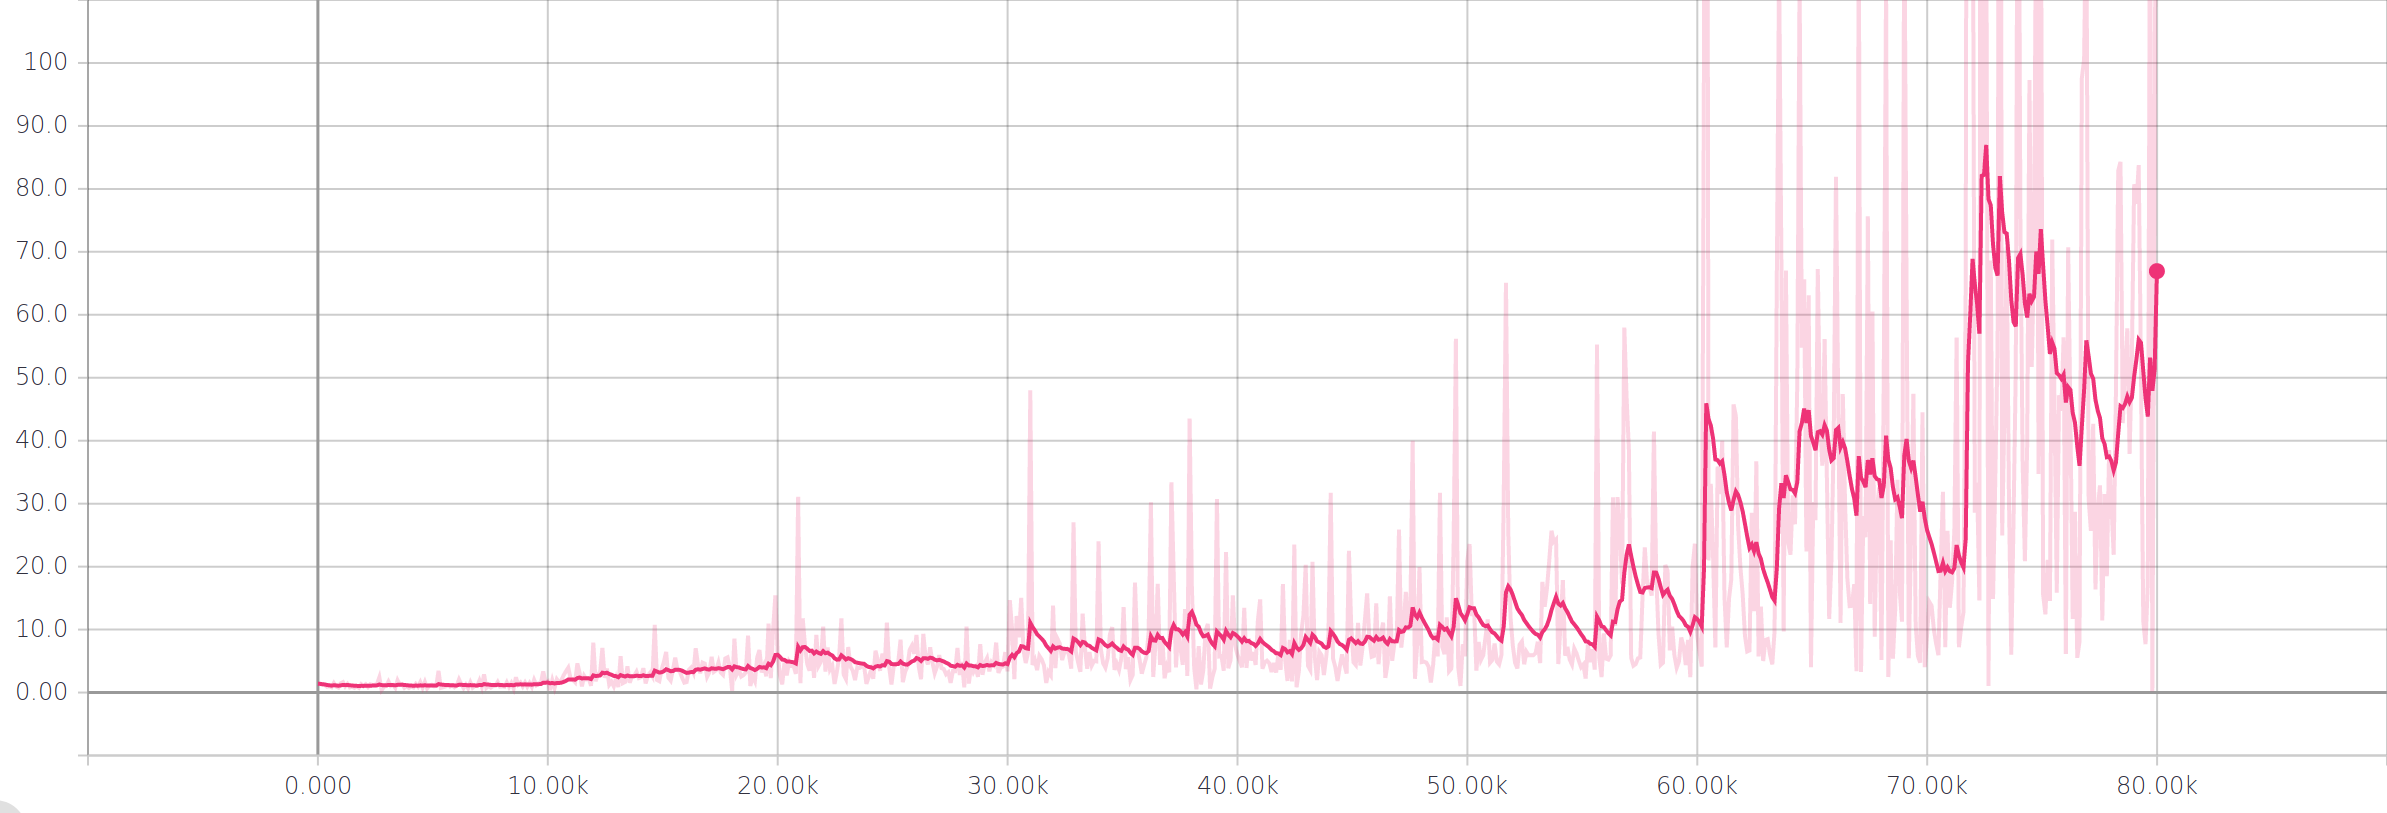
\includegraphics[width=1\textwidth, clip]{ACGAN-Gen-Loss}
  \label{fig:ACGAN-Gen-Loss}%
\end{figure}
%
\newline
The best results with the auxiliary classifier were achieved with a learning rate of 1e-3, faster than was possible with the baseline WGAN, and a generator to discriminator update ratio of 2 to 1.
This trial run also had label smoothing applied to the labels being compared in the discriminator loss function.
\newline
%
\begin{figure}[ht]%
  \caption{The discriminator loss for ACGAN}
  \centering
  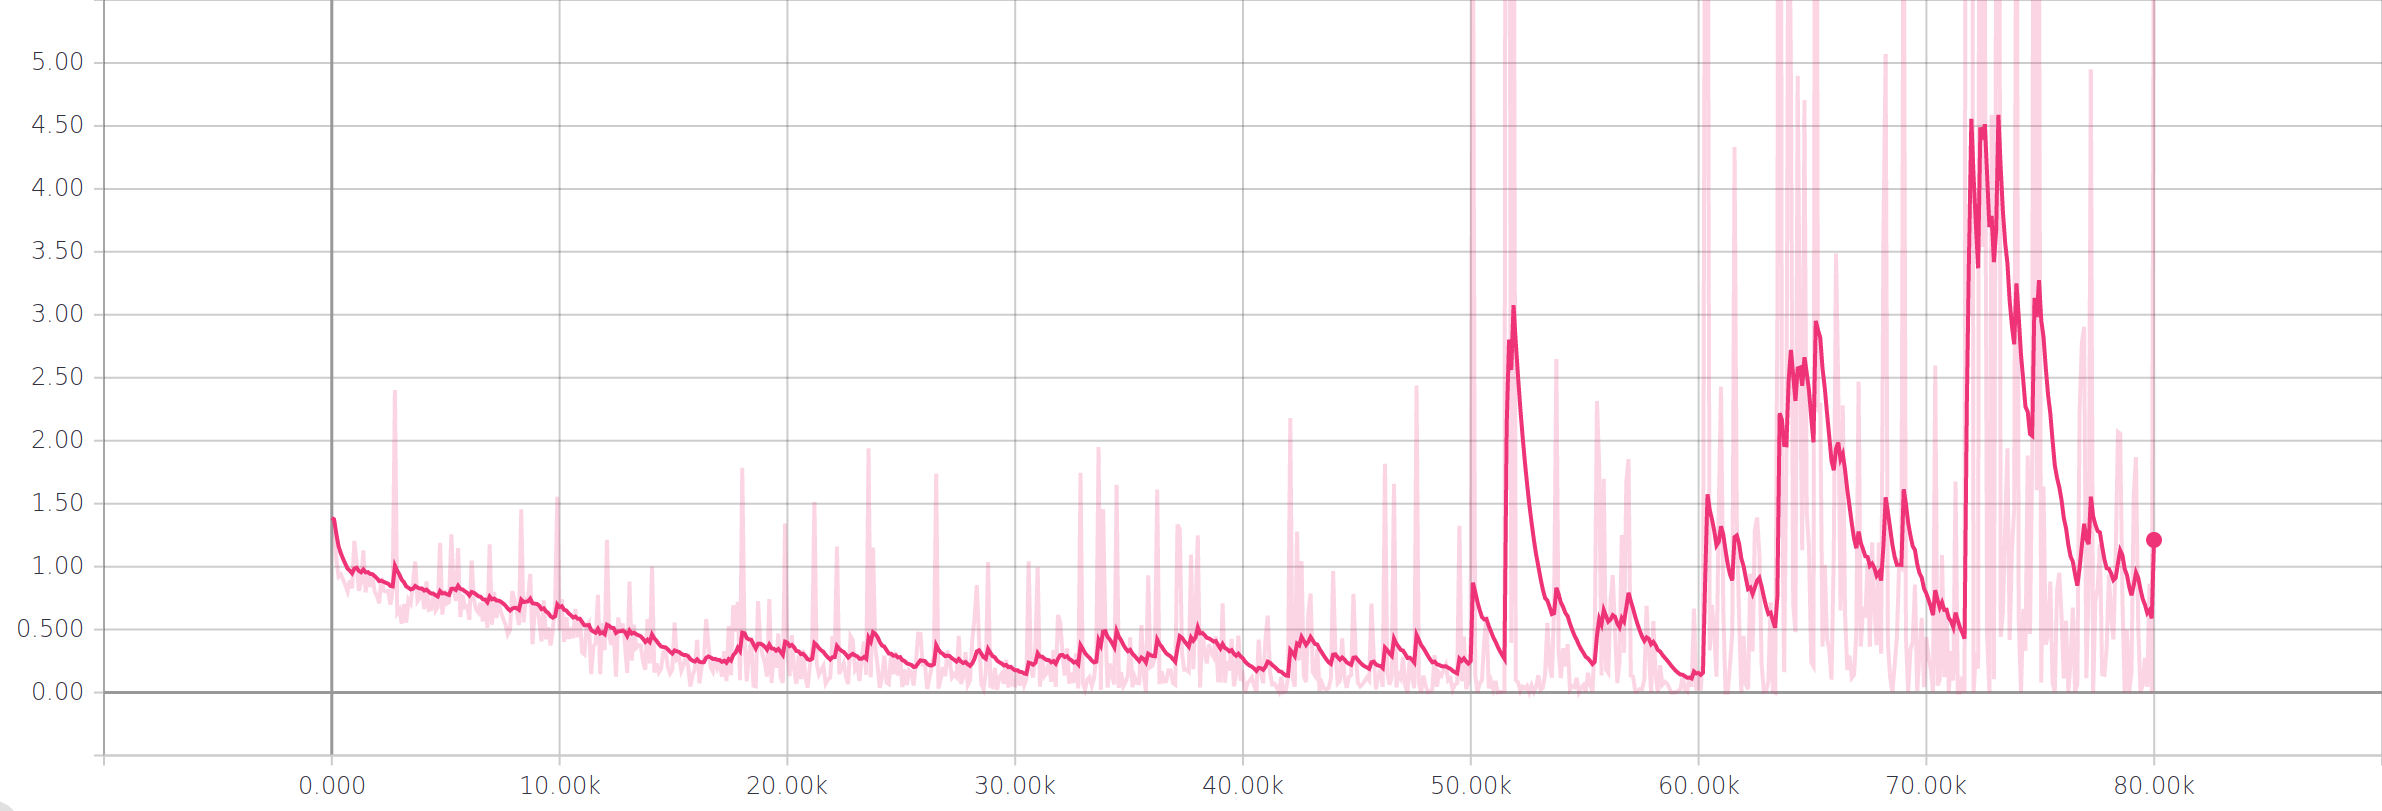
\includegraphics[width=1\textwidth, clip]{ACGAN-Dis-Loss}
  \label{fig:ACGAN-Dis-Loss}%
\end{figure}
%
\newline
The results from this experiment showed that two modes of data were being generated but there was very little variability within those modes.
This would seem to be a form of manifold mode collapse as the discrete modes are still being generated but only a very narrow range of each manifold is generated.
The two generated samples in Figure \ref{fig:ACGAN-Waves} are representative of nearly all the samples being generated.
\newline
%
\begin{figure}[ht]%
    \centering
    \subfloat[Generated]{{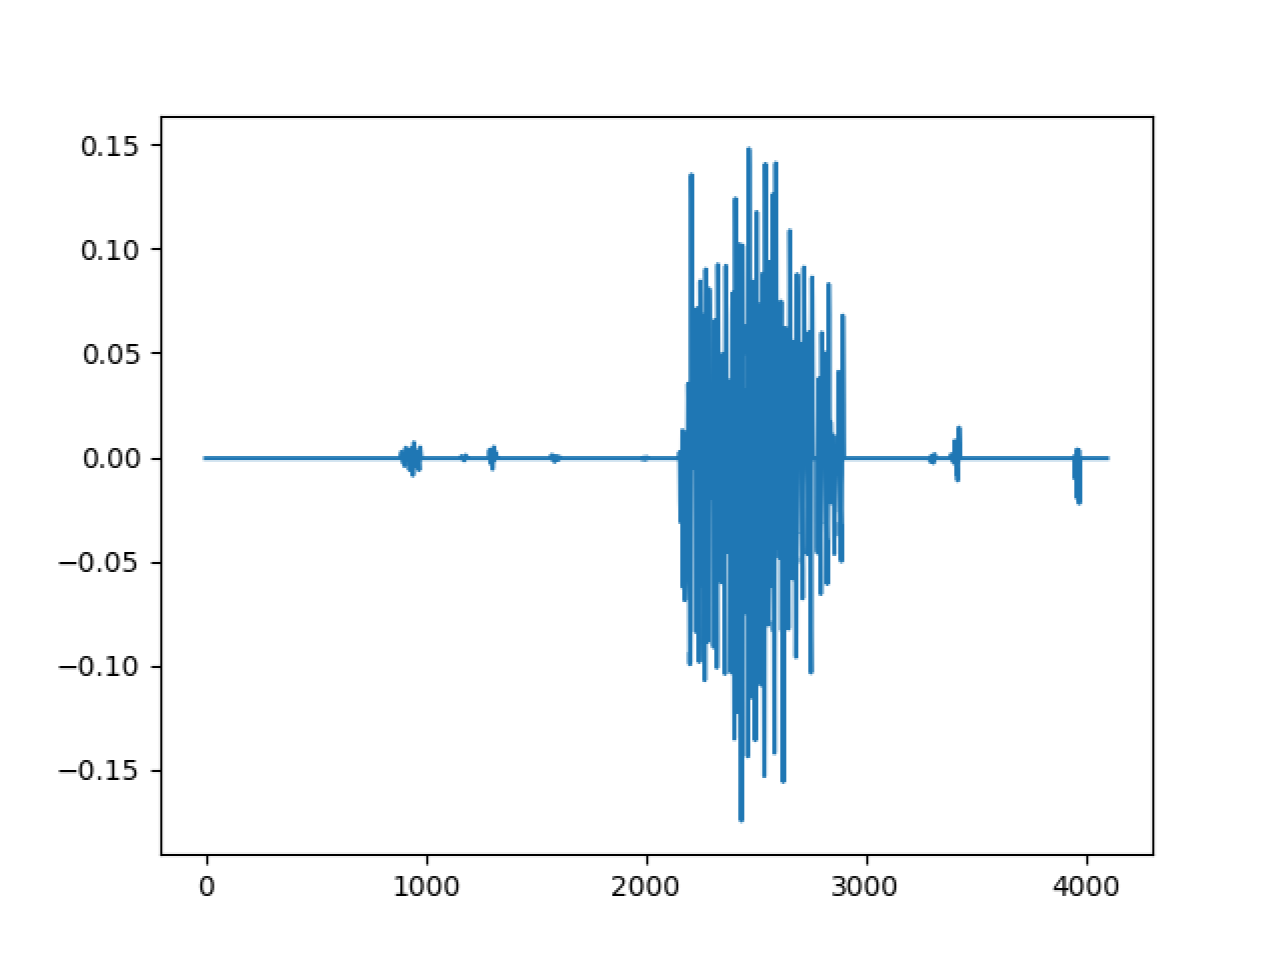
\includegraphics[width=5cm]{ACGAN-GenWave1} }}%
    \qquad
    \subfloat[Generated]{{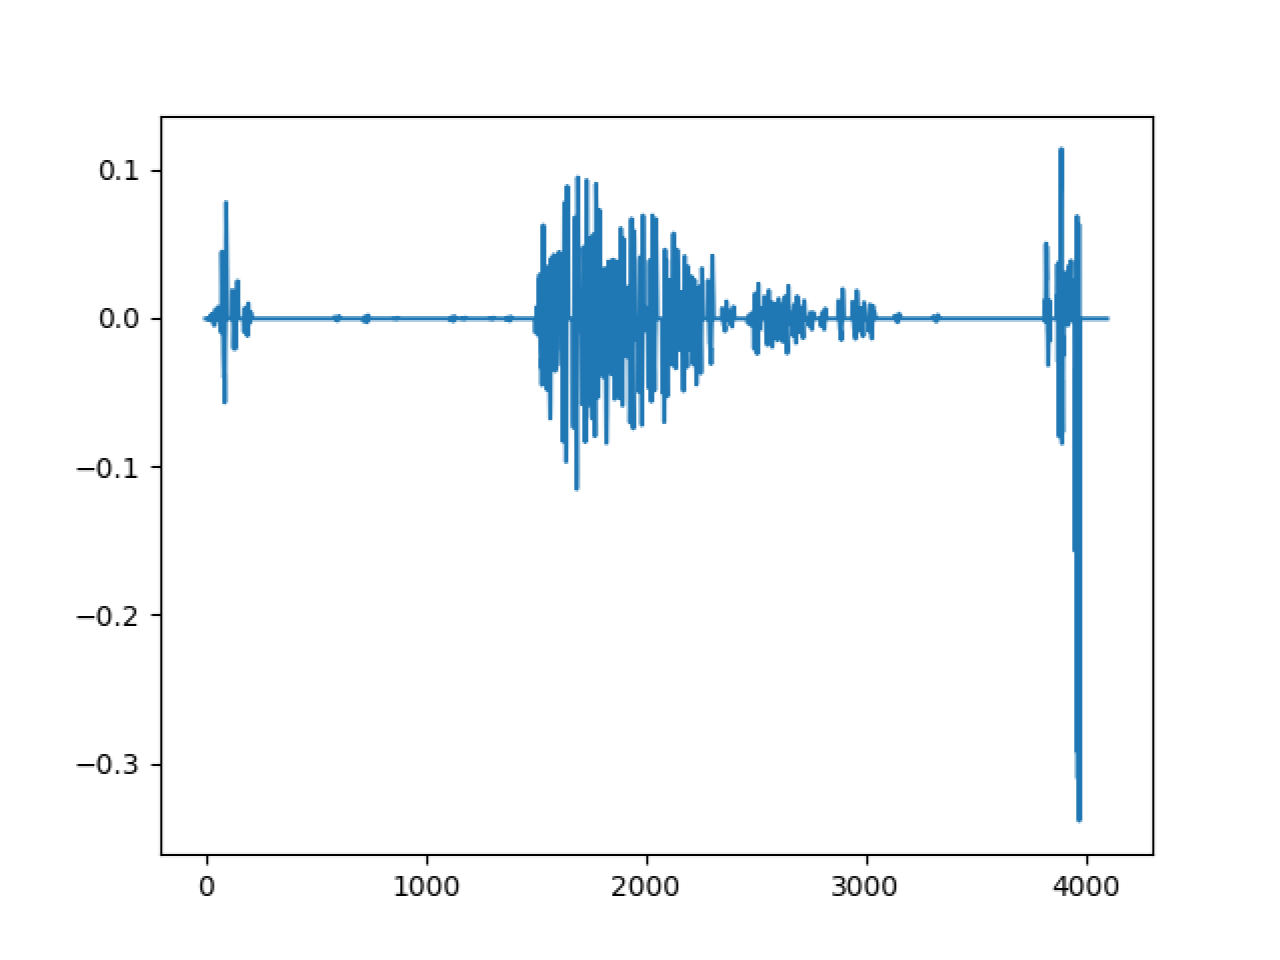
\includegraphics[width=5cm]{ACGAN-GenWave2} }}%
    \qquad
    \subfloat[Real]{{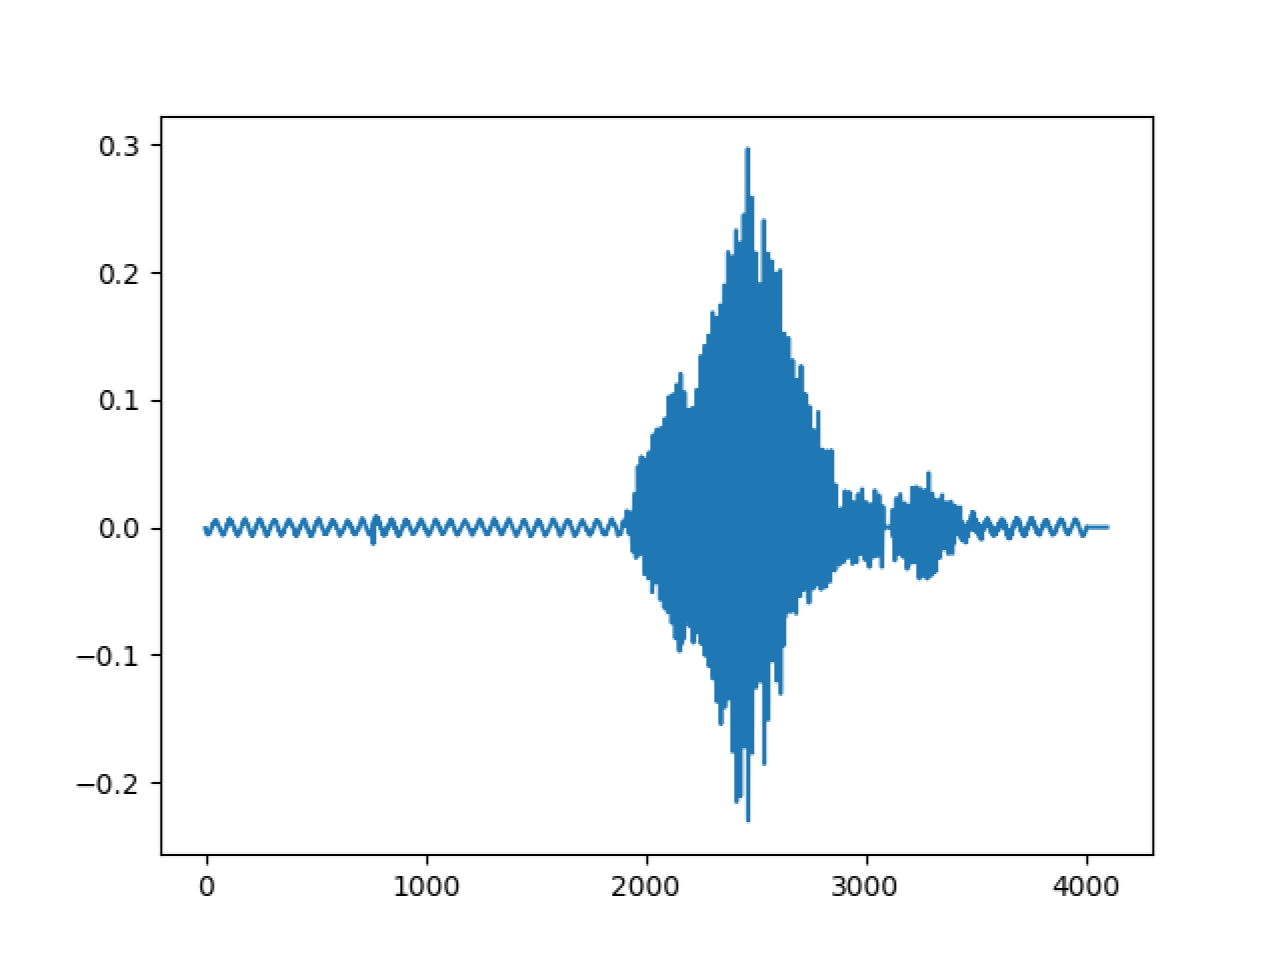
\includegraphics[width=5cm]{ACGAN-RealWave1} }}%
    \qquad
    \subfloat[Real]{{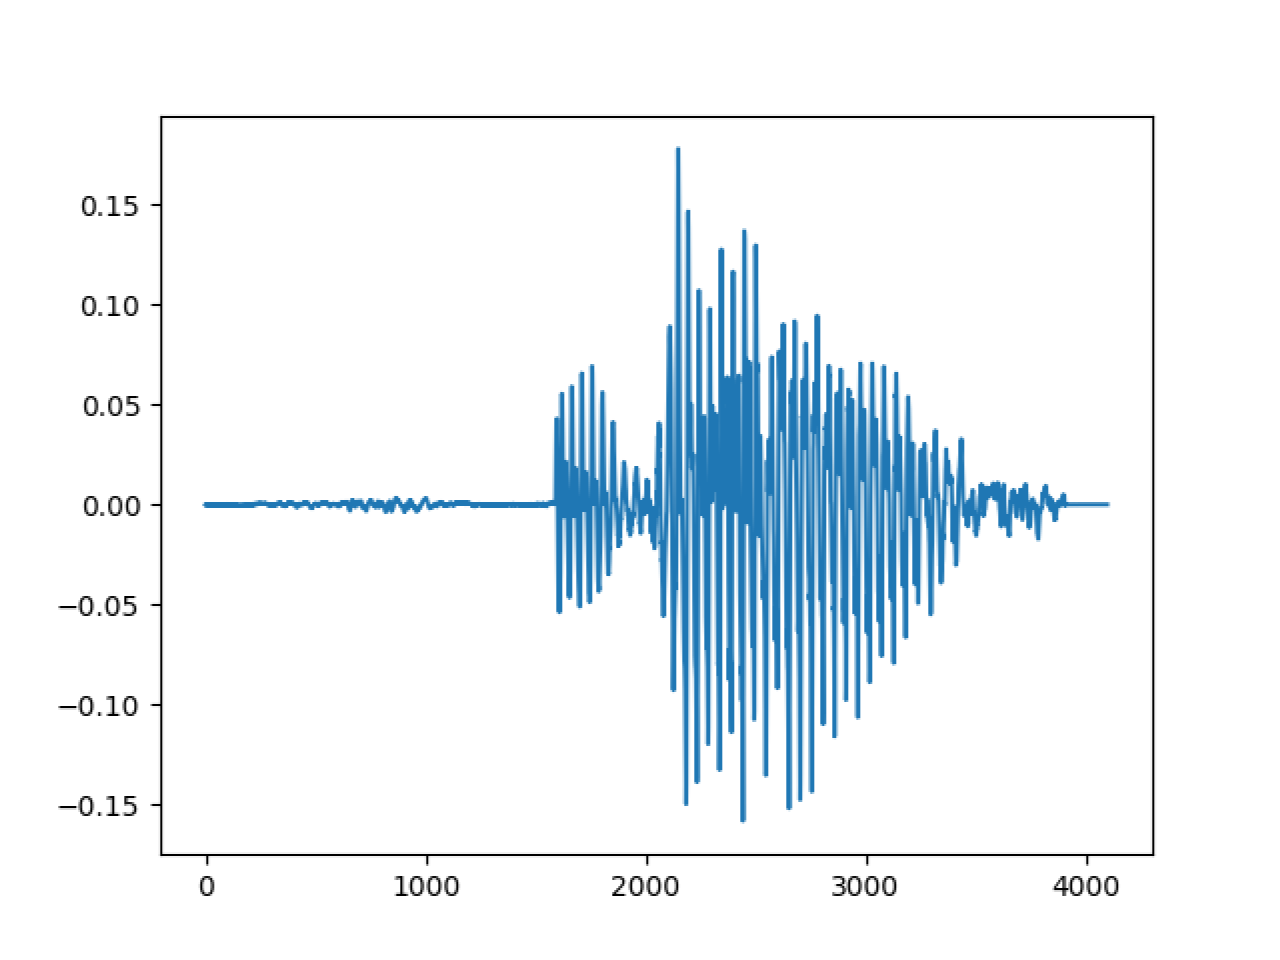
\includegraphics[width=5cm]{ACGAN-RealWave2} }}%
    \caption{Wave plots of ACGAN generated and real samples}%
    \label{fig:ACGAN-Waves}%
\end{figure}
%
\newline
While the amplitude of the generated waveforms seems superficially similar to those of the real data samples, the spectogram plots in Figure \ref{fig:ACGAN-Specs} show that the relationships between the frequencies over time have not been captured in a sophisticated manner.
%
\newline
\begin{figure}[ht]%
    \centering
    \subfloat[Generated]{{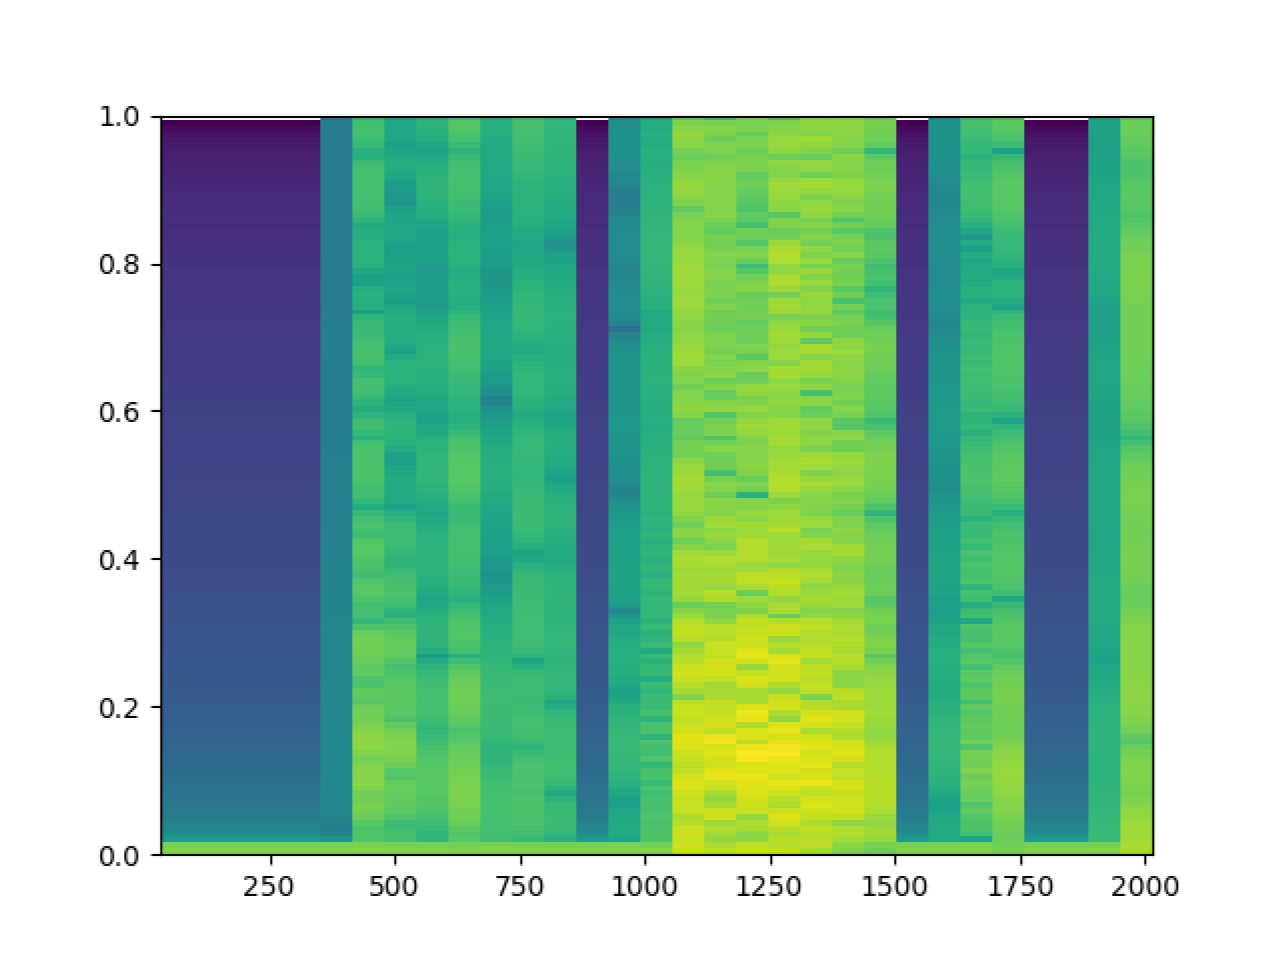
\includegraphics[width=5cm]{ACGAN-GenSpec1} }}%
    \qquad
    \subfloat[Generated]{{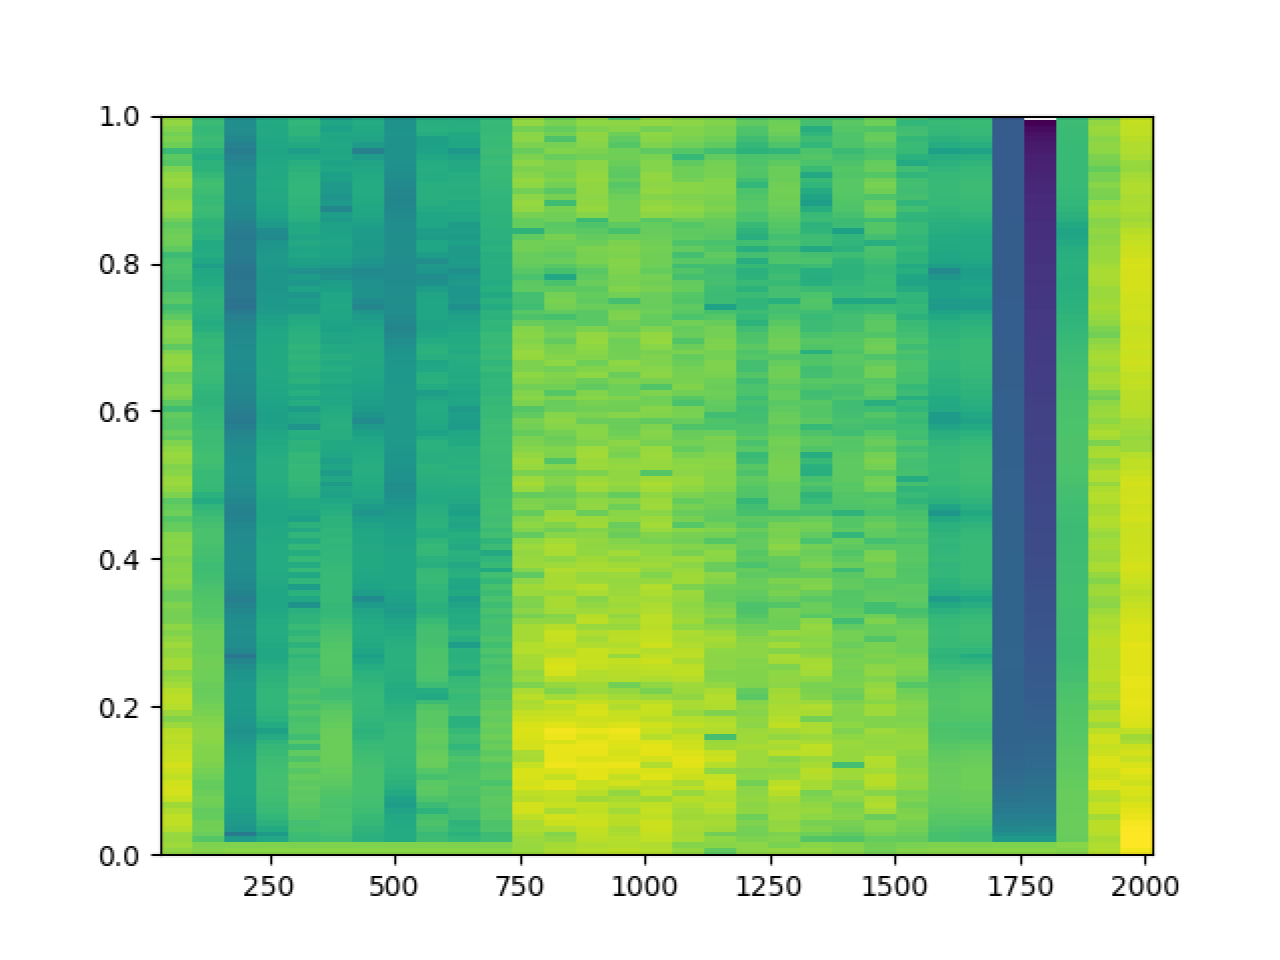
\includegraphics[width=5cm]{ACGAN-GenSpec2} }}%
    \qquad
    \subfloat[Real]{{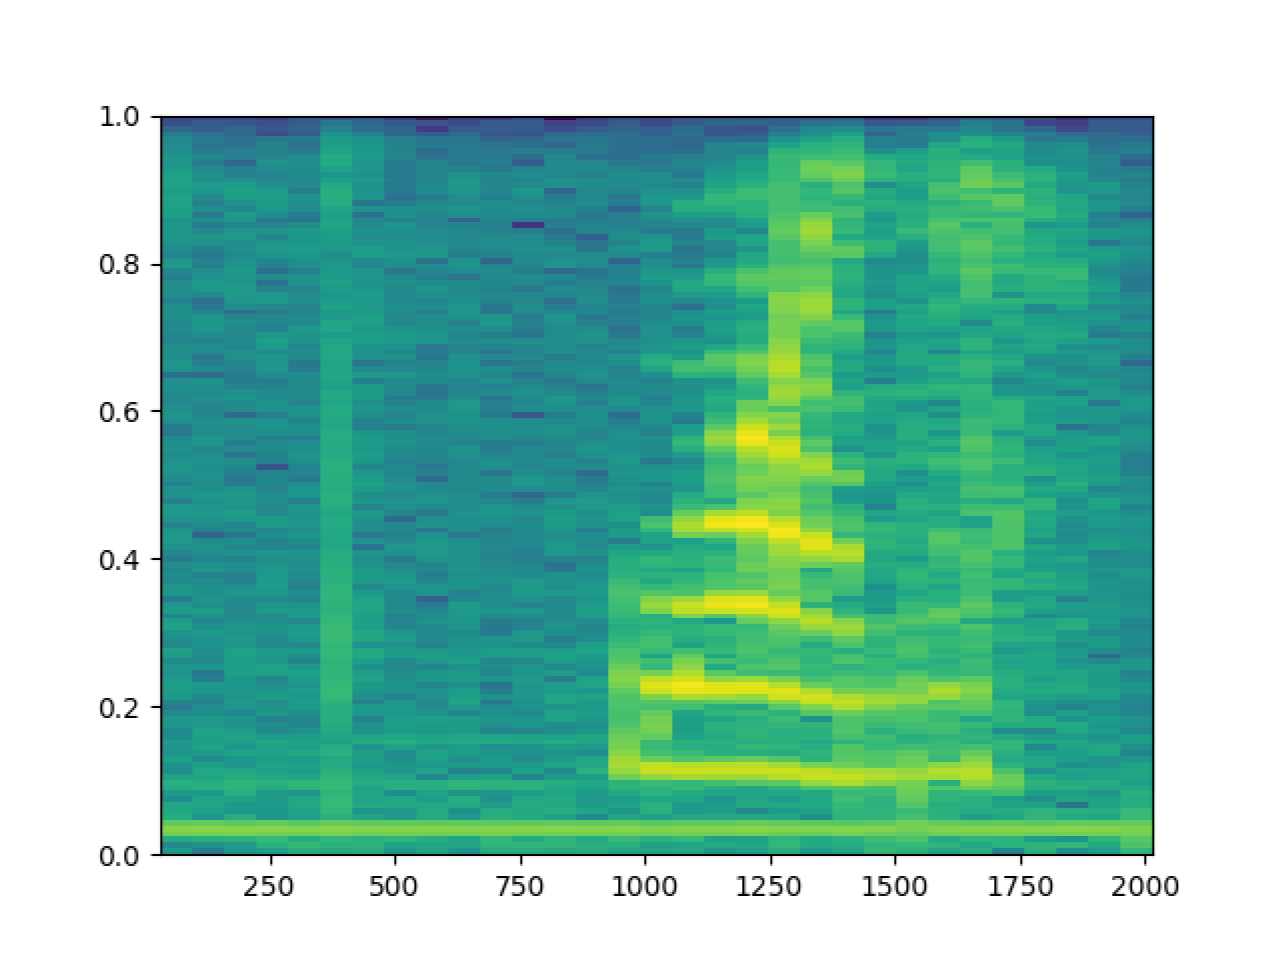
\includegraphics[width=5cm]{ACGAN-RealSpec1} }}%
    \qquad
    \subfloat[Real]{{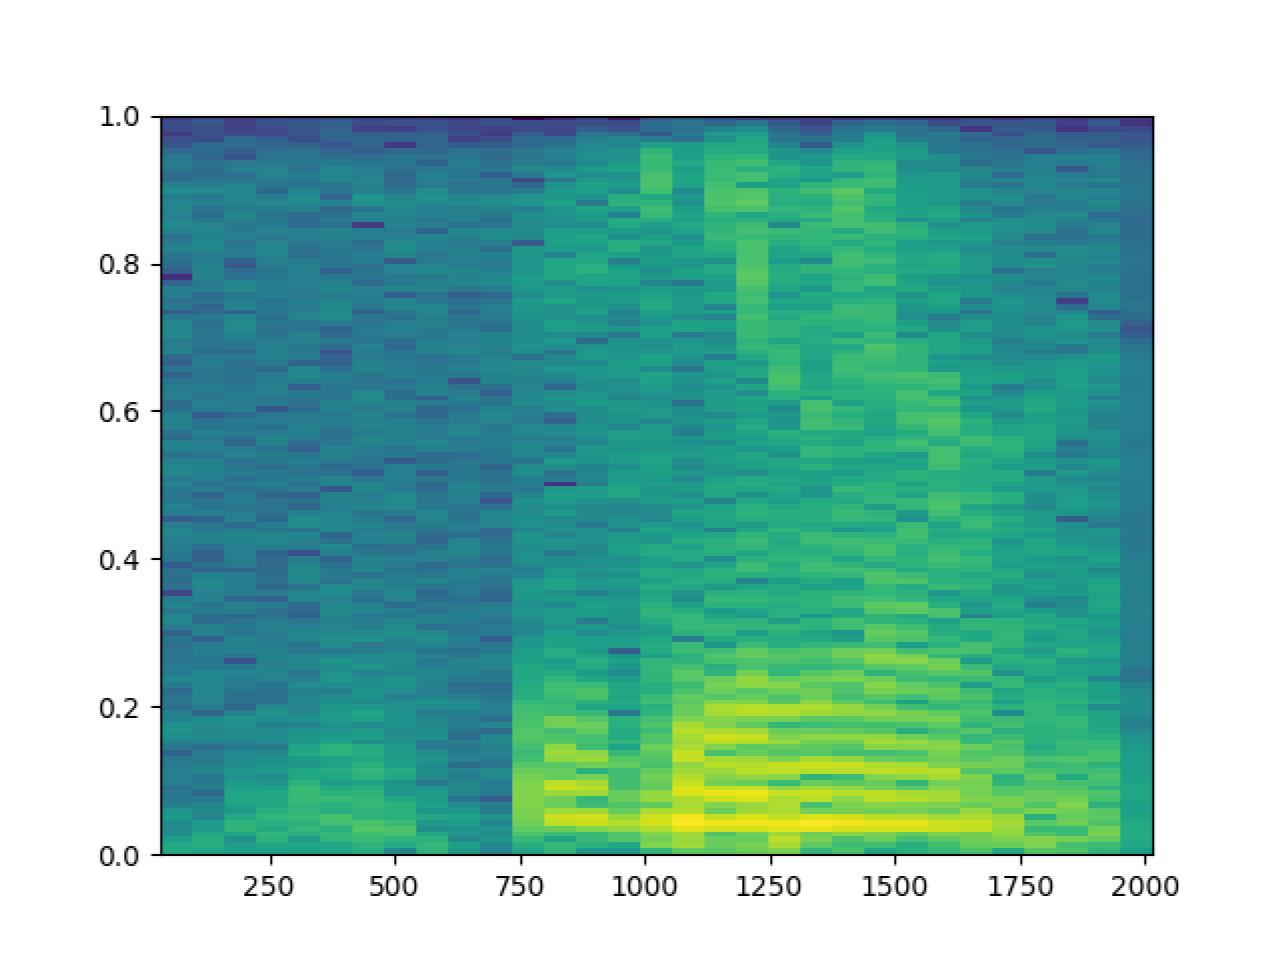
\includegraphics[width=5cm]{ACGAN-RealSpec2} }}%
    \caption{Spectograms of ACGAN generated and real samples}%
    \label{fig:ACGAN-Specs}%
\end{figure}
%
\clearpage

\section{Conclusion}

WaveGAN is a difficult model to replicate and train to convergence; the hyperparameters reported by \citeauthor{2018arXiv180204208D} do not result in successful training with downsized models and the search for a working set of hyperparameters required a large amount of testing.
A greater budget would have allowed the replication of the original WaveGAN experiment and may have freed time to focus on finding the correct architecture and hyperparameters for a conditional model.
\newline
\newline
The project did however reveal that there are difficulties modifying the number of layers in the WaveGAN model and this way have an impact on the feasibility of designing a WaveGAN with the capability of generating audio of arbitrary lengths.
Further research is needed into the relationship between the number of layers in the model, the number of filters that are used in the convolution layers, and the values of hyperparameters that result in convergence.
\newline
\newline
Designing and training a conditional WaveGAN model upon the already unstable downsized WaveGAN model required significant testing of variations in the architecture and hyperparameters.
Two different methods of conditioning were attempted with variations on the cost functions used and with the addition of noise to the discriminator input and label smoothing in the cost functions.
Further attempts at producing a stable conditional WaveGAN are not recommended without first researching further the problems with the implementation of the baseline WaveGAN. 
\newline
\newline
Nevertheless, we can at least state that the concatenation method of conditioning is unlikely to be the simplest to develop into a stable functioning model; even extreme values for the parameters had little impact on the time taken for the loss to diverge.
The auxiliary classifier method of conditioning showed some promise, even though it was not entirely successful within the limitations of the experiment; a better understanding of the relationship between the original and downsized WaveGAN models will hopefully give an insight into how this method may be improved so as to avoid mode collapse and train more quickly.
\newline
\newline
During the testing of the concatenation method of conditioning there was an attempt at bypassing the one-hot style embedding layer and instead placing the audio wave data directly into a channel to label the class of data being passed in as a parameter.
This is a minor change to the simple concatenation of the embedding layers onto the original data but monitoring showed that this seemed to result in faster training with the generated waveforms taking a form similar to that of the real data more quickly.
A minor program of research to review previous conditional \ac{GAN} experiments and compare results generated with this new method may be worthwhile.

\newpage

% Bibliography
\setlength{\bibhang}{0pt}
\bibliography{Bibliography}
\bibliographystyle{agsm}

\newpage

% Appendix
\begin{appendices}

  % Code font
  \lstset{
    basicstyle=\footnotesize\ttfamily,
    breaklines=true
  }

  \section{Development Environment}

  \subsection{Software}

  \subsubsection{Tensorflow}

  Tensorflow (version 1.9.0) is an open source machine learning framework created by Google with an emphasis on the design and training of graph models, particularly neural networks.
  The discriminator and generator models for this project were both written and run with TensorFlow.

  \subsubsection{Tensorboard}

  Tensorboard (version version 1.9.0) is a visualization dashboard tool built to accompany Tensorflow that allows for live monitoring of experiments.
  A number of features of Tensorboard was greatly important in the training of the models used in this project; particularly the ability to monitor the discriminator and generator loss, visualize the plotted output of the audio samples; and also listen to the audio samples as they are being generated. 

  \subsubsection{Python}

  All code was written in Python (version 3.6.5.) while utilising a number of libraries, such as: NumPy (version 1.13.3), a library allowing more efficient writing of code for processing array; (version Librosa 0.6.0), a library for the processing and plotting of digital audio; (version Soundfile 0.10.1), another library for audio processing; and matplotlib, a visualization library.
  \newline
  \newline
  Another library tf-matplotlib was imported to allow integration between Tensorboard and matplotlib, a mathematical plotting library for Python.
  This library allows for diverse and richer plotting functions than is currently available within TensorBoard to be visualized during training.
  It is itself dependent on the library matplotlib (version 2.2.0).

  \subsection{Cloud Infrastructure}

  The original WaveGAN model implemented by \citeauthor{2018arXiv180204208D} required four days of training with a top-of-the-range NVIDIA Tesla P100 GPU.
  At the time of writing, this GPU is available from Amazon for US \$5,500, beyond an acceptable budget for a student project.
  Without physical access to a powerful GPU the experiments were instead run on cloud service GPUs.

  \subsubsection{Amazon EC2}

  Amazon Elastic Compute Cloud 2 is a web service that providing computing power in the cloud.
  Users have a choice over the development environment that they want to use in the cloud; these are called Amazon Machine Images (AMIs)
  AMIs exist for common tasks; the Ubuntu Deep Learning AMI used for these experiments provides a Ubuntu server interface, Tensorflow, Tensorboard, CUDA and Python.
  \newline
  \newline
  AWS also includes the choice of 'instances' which are physical configurations of GPUs that the user can compute with.
  The 'instance' type used for these experiments was the p2.xlarge instance which gives access to only a single GPU, an NVIDIA K80 GPU.

  \newpage

  \section{Instructions for Using the Software}

  There are two programs; the first prepares data for training; and the second is for training the model, testing hyperparameters and generating data.

  \subsection{Data Preparation}

  Preparation of the data takes place through the command line by calling the file 'Downsampler.py'.
  \newline
  \newline
  The first command is 'divider' which can accept values of '1', '4', and '16'; this commands the program to divide the sample rate of approximately 16k with either of these numbers to obtain a downsampled dataset.
  \newline
  \newline
  The second and third commands 'inPath' and 'outPath' accept the path where your data is held and the path where you would like to save your downsampled data.
  \newline
  \newline
  The third command is 'words' which takes a list of strings representing the words from the \ac{SC09} dataset that will be downsampled; the default is 'zero' and 'one'.
  \newline
  \newline
  Following is an example of how to use this command:
  \newline
\begin{lstlisting}[language=bash]
    python3 Downsampler.py 4 '/path/to/my/data/' '/path//I/am/downsampling/to/'
\end{lstlisting}

  \subsection{Training and Generating}

  Training and generation with the models is through the command line by calling the file 'Manager.py'.
  \newline
  \newline
  The 'mode' command tells the program whether it should 'train' or 'gen' (generate data).
  \newline
  \newline
  The 'model' command tells the program whether to train or generate from a 'WGAN' (WaveGAN), 'CWGAN' (concatenated WaveGAN), or 'ACGAN' (auxiliary classifier GAN).
  \newline
  \newline
  The 'wave' command tells the program which wave length (sample size) to use, default is 4096.
  \newline
  \newline
  The 'runName' argument gives an extra textual name by which the trained model can be identified.
  \newline
  \newline
  The 'checkpointNum' argument tells the program which checkpoint to use when generating new samples.
  \newline
  \newline
  The 'genMode' argument tells the program which mode of the data to generate samples from when generation is through a conditional model.
  \newline
  \newline
  The 'genLength' argument tell the generator how many samples to generate; the default is 100.
  \newline
  \newline
  The 'lamb' argument pass the gradient penalty lambda number to the Wasserstein loss; the default is 10.
  \newline
  \newline
  The 'batch' argument tells the program which batch size to use during model training; the default is 64.
  \newline
  \newline
  The 'iterations' argument tells the program how many iterations through batches need to be completed before training is complete.
  \newline
  \newline
  The 'D\_updates' argument tells the program how many updates to the discriminator should take place per iteration; the default is 1.
  \newline
  \newline
  The 'G\_updates' argument tells the program how many updates to the generator should take place per iteration; the default is 1.
  \newline
  \newline
  The 'learnRate' argument passes a learning rate into the Adam optimizer; the default is 0.0001.
  \newline
  \newline
  The 'words' argument accepts a list of words to include in the training; the default is 'zero' and 'one'.
  \newline
  \newline
  An example of a command that would train the model:
  \newline
  \begin{lstlisting}[language=bash]
  python3 Manager.py -mode=train -model=WGAN -wave=4096 -iterations=2 -lamb=10 -D_updates=1 -G_updates=1 -runName=TestA -batch=64 -learnRate=0.0001 -words zero one
\end{lstlisting}
  %
  An example of a command that generate from the model created with the previous command:
  \newline
  \begin{lstlisting}[language=bash]
  python3 Manager.py -mode=gen -model=WGAN -wave=4096 -checkpointNum=0 -genLength=100 -runName=TestA
\end{lstlisting}

  \newpage

  \section{Model Architecture Tables}

  \subsection{WaveGAN}

  \begin{table}[ht]
    
    \caption{Layers of the WGAN Discriminator}
    \label{tab:WGAN_Dis}
    
    \begin{center}
      \begin{tabular}{ l | l | l}
        
        Operation & Kernel Size & Output Shape \\
        \hline
        Input {\it x} or {\it G}({\it z}) & & ({\it n}, 4096, 1) \\
        % to 1024
        Conv1D (Stride=4) & (25, {\it d}, 2{\it d}) & ({\it n}, 1024, 32) \\
        LReLU (\textalpha \, = 0.2) & & ({\it n}, 1024, 32) \\
        Phase Shuffle ({\it n} = 2) & & ({\it n}, 1024, 32) \\
        % to 256
        Conv1D (Stride=4) & (25, 2{\it d}, 4{\it d}) & ({\it n}, 256, 64) \\
        LReLU (\textalpha \, = 0.2) & & ({\it n}, 256, 64) \\
        Phase Shuffle ({\it n} = 2) & & ({\it n}, 256, 64) \\
        % to 64
        Conv1D (Stride=4) & (25, 4{\it d}, 8{\it d}) & ({\it n}, 64, 128) \\
        LReLU (\textalpha \, = 0.2) & & ({\it n}, 64, 128) \\
        Phase Shuffle ({\it n} = 2) & & ({\it n}, 64, 128) \\
        % to 16
        Conv1D (Stride=4) & (25, 8{\it d}, 16{\it d}) & ({\it n}, 16, 256) \\
        LReLU (\textalpha \, = 0.2) & & ({\it n}, 16, 256) \\
        % Output
        Reshape & & ({\it n}, 4096) \\
        Dense & (4096, 1) & ({\it n}, 1)\\
        
      \end{tabular}
    \end{center}
    
  \end{table}

  \begin{table}[ht]
    
    \caption{Layers of the WGAN Generator}
    \label{tab:WGAN_Gen}
    
    \begin{center}
      \begin{tabular}{ l | l | l}
        
        Operation & Kernel Size & Output Shape \\
        \hline
        Input {\it z} $\sim$ Uniform(-1, 1) & & ({\it n}, 100) \\
        Dense 1 & (100, 4096) & ({\it n}, 4096) \\
        Reshape & & ({\it n}, 16, 256) \\
        %
        ReLU & & ({\it n}, 16, 256) \\
        Trans Conv1D (Stride=4) & (25, 8{\it d}, 4{\it d}) & ({\it n}, 64, 128) \\
        %
        ReLU & & ({\it n}, 64, 128) \\
        Trans Conv1D (Stride=4) & (25, 4{\it d}, 2{\it d}) & ({\it n}, 256, 64) \\
        %
        ReLU & & ({\it n}, 256, 64) \\
        Trans Conv1D (Stride=4) & (25, 2{\it d}, {\it d}) & ({\it n}, 1024, 32) \\
        %
        ReLU & & ({\it n}, 1024, 32) \\
        Trans Conv1D (Stride=4) & (25, {\it d}, {\it c}) & ({\it n}, 4096, 1) \\
        Tanh & & ({\it n}, 4096, 1) \\

      \end{tabular}
    \end{center}
    
  \end{table}

  \clearpage

  \subsection{Conditional WaveGAN with Concatenation}

  \begin{table}[ht]
    
    \caption{Layers of the Concatenated Conditional WaveGAN Discriminator}
    \label{tab:CWGAN_Dis}
    
    \begin{center}
      \begin{tabular}{ l | l | l}
        
        Operation & Kernel Size & Output Shape \\
        \hline
        Concat {\it x} and {\it y} & & ({\it n}, 4096, 3) \\
        % to 1024
        Conv1D (Stride=4) & (25, {\it d}, 2{\it d}) & ({\it n}, 1024, 32) \\
        LReLU (\textalpha \, = 0.2) & & ({\it n}, 1024, 32) \\
        Phase Shuffle ({\it n} = 2) & & ({\it n}, 1024, 32) \\
        % to 256
        Conv1D (Stride=4) & (25, 2{\it d}, 4{\it d}) & ({\it n}, 256, 64) \\
        LReLU (\textalpha \, = 0.2) & & ({\it n}, 256, 64) \\
        Phase Shuffle ({\it n} = 2) & & ({\it n}, 256, 64) \\
        % to 64
        Conv1D (Stride=4) & (25, 4{\it d}, 8{\it d}) & ({\it n}, 64, 128) \\
        LReLU (\textalpha \, = 0.2) & & ({\it n}, 64, 128) \\
        Phase Shuffle ({\it n} = 2) & & ({\it n}, 64, 128) \\
        % to 16
        Conv1D (Stride=4) & (25, 8{\it d}, 16{\it d}) & ({\it n}, 16, 256) \\
        LReLU (\textalpha \, = 0.2) & & ({\it n}, 16, 256) \\
        % Output
        Conv1D (Stride=1) & (16, 16, 256) & ({\it n}, 1, 1) \\
        
      \end{tabular}
    \end{center}
    
  \end{table}

  \begin{table}[ht]
    
    \caption{Layers of the Concatenated Conditional WaveGAN Generator}
    \label{tab:ACGAN_Gen}
    
    \begin{center}
      \begin{tabular}{ l | l | l}
        
        Operation & Kernel Size & Output Shape \\
        \hline
        Dense & (100, 4096) & ({\it n}, 4094) \\
        Reshape {\it as z} & & ({\it n}, 16, 254) \\
        Concat {\it z} and {\it y} & & ({\it n}, 1, 4096) \\
        %
        ReLU & & ({\it n}, 1, 4096) \\
        Trans Conv1D (Stride=1) & (16, 8{\it d}, 4{\it d}) & ({\it n}, 16, 256) \\
        %
        ReLU & & ({\it n}, 16, 256) \\
        Trans Conv1D (Stride=4) & (25, 8{\it d}, 4{\it d}) & ({\it n}, 64, 128) \\
        %
        ReLU & & ({\it n}, 64, 128) \\
        Trans Conv1D (Stride=4) & (25, 4{\it d}, 2{\it d}) & ({\it n}, 256, 64) \\
        %
        ReLU & & ({\it n}, 256, 64) \\
        Trans Conv1D (Stride=4) & (25, 2{\it d}, {\it d}) & ({\it n}, 1024, 32) \\
        %
        ReLU & & ({\it n}, 1024, 32) \\
        Trans Conv1D (Stride=4) & (25, {\it d}, {\it c}) & ({\it n}, 4096, 1) \\
        Tanh & & ({\it n}, 4096, 1) \\

      \end{tabular}
    \end{center}
    
  \end{table}

  \clearpage

  \subsection{Conditional WaveGAN with Auxiliary Classifier}

  \begin{table}[ht]
    
    \caption{Layers of the Auxiliary Classifier Conditional WaveGAN Discriminator}
    \label{tab:ACGAN_Dis}
    
    \begin{center}
      \begin{tabular}{ l | l | l}
        
        Operation & Kernel Size & Output Shape \\
        \hline
        % to 1024
        Conv1D (Stride=4) & (25, {\it d}, 2{\it d}) & ({\it n}, 1024, 32) \\
        LReLU (\textalpha \, = 0.2) & & ({\it n}, 1024, 32) \\
        Phase Shuffle ({\it n} = 2) & & ({\it n}, 1024, 32) \\
        % to 256
        Conv1D (Stride=4) & (25, 2{\it d}, 4{\it d}) & ({\it n}, 256, 64) \\
        LReLU (\textalpha \, = 0.2) & & ({\it n}, 256, 64) \\
        Phase Shuffle ({\it n} = 2) & & ({\it n}, 256, 64) \\
        % to 64
        Conv1D (Stride=4) & (25, 4{\it d}, 8{\it d}) & ({\it n}, 64, 128) \\
        LReLU (\textalpha \, = 0.2) & & ({\it n}, 64, 128) \\
        Phase Shuffle ({\it n} = 2) & & ({\it n}, 64, 128) \\
        % to 16
        Conv1D (Stride=4) & (25, 8{\it d}, 16{\it d}) & ({\it n}, 16, 256) \\
        LReLU (\textalpha \, = 0.2) & & ({\it n}, 16, 256) \\
        % Output
        \hline
        Conv1D (Stride=1) & (16, 16, 256) & ({\it n}, 1, 1) \\
        \hline
        Flatten & (64, 16, 256) & ({\it n}, 4096) \\
        Dense & (4096) & ({\it n}, 2) \\
        
      \end{tabular}
    \end{center}
    
  \end{table}

  \begin{table}[ht]
    
    \caption{Layers of the Auxiliary Classifier Conditional WaveGAN Generator}
    \label{tab:CWGAN_Gen}
    
    \begin{center}
      \begin{tabular}{ l | l | l}
        
        Operation & Kernel Size & Output Shape \\
        \hline
        Dense & (100, 4096) & ({\it n}, 4094) \\
        Reshape {\it as z} & & ({\it n}, 16, 254) \\
        Concat {\it z} and {\it y} & & ({\it n}, 1, 4096) \\
        %
        ReLU & & ({\it n}, 1, 4096) \\
        Trans Conv1D (Stride=1) & (16, 8{\it d}, 4{\it d}) & ({\it n}, 16, 256) \\
        %
        ReLU & & ({\it n}, 16, 256) \\
        Trans Conv1D (Stride=4) & (25, 8{\it d}, 4{\it d}) & ({\it n}, 64, 128) \\
        %
        ReLU & & ({\it n}, 64, 128) \\
        Trans Conv1D (Stride=4) & (25, 4{\it d}, 2{\it d}) & ({\it n}, 256, 64) \\
        %
        ReLU & & ({\it n}, 256, 64) \\
        Trans Conv1D (Stride=4) & (25, 2{\it d}, {\it d}) & ({\it n}, 1024, 32) \\
        %
        ReLU & & ({\it n}, 1024, 32) \\
        Trans Conv1D (Stride=4) & (25, {\it d}, {\it c}) & ({\it n}, 4096, 1) \\
        Tanh & & ({\it n}, 4096, 1) \\

      \end{tabular}
    \end{center}
    
  \end{table}

  \clearpage

  \section{Model Graphs}

  The following pages contain the graph structures for the baseline and conditional WaveGAN models as displayed through Tensorboard.
  The 'Main Graph' segments show the high level architecture of the models; the 'Auxiliary Nodes' segments show the names and structures of various other components.

  \begin{figure}[ht]
    \caption{WaveGAN Model Main Graph}
    \centering
    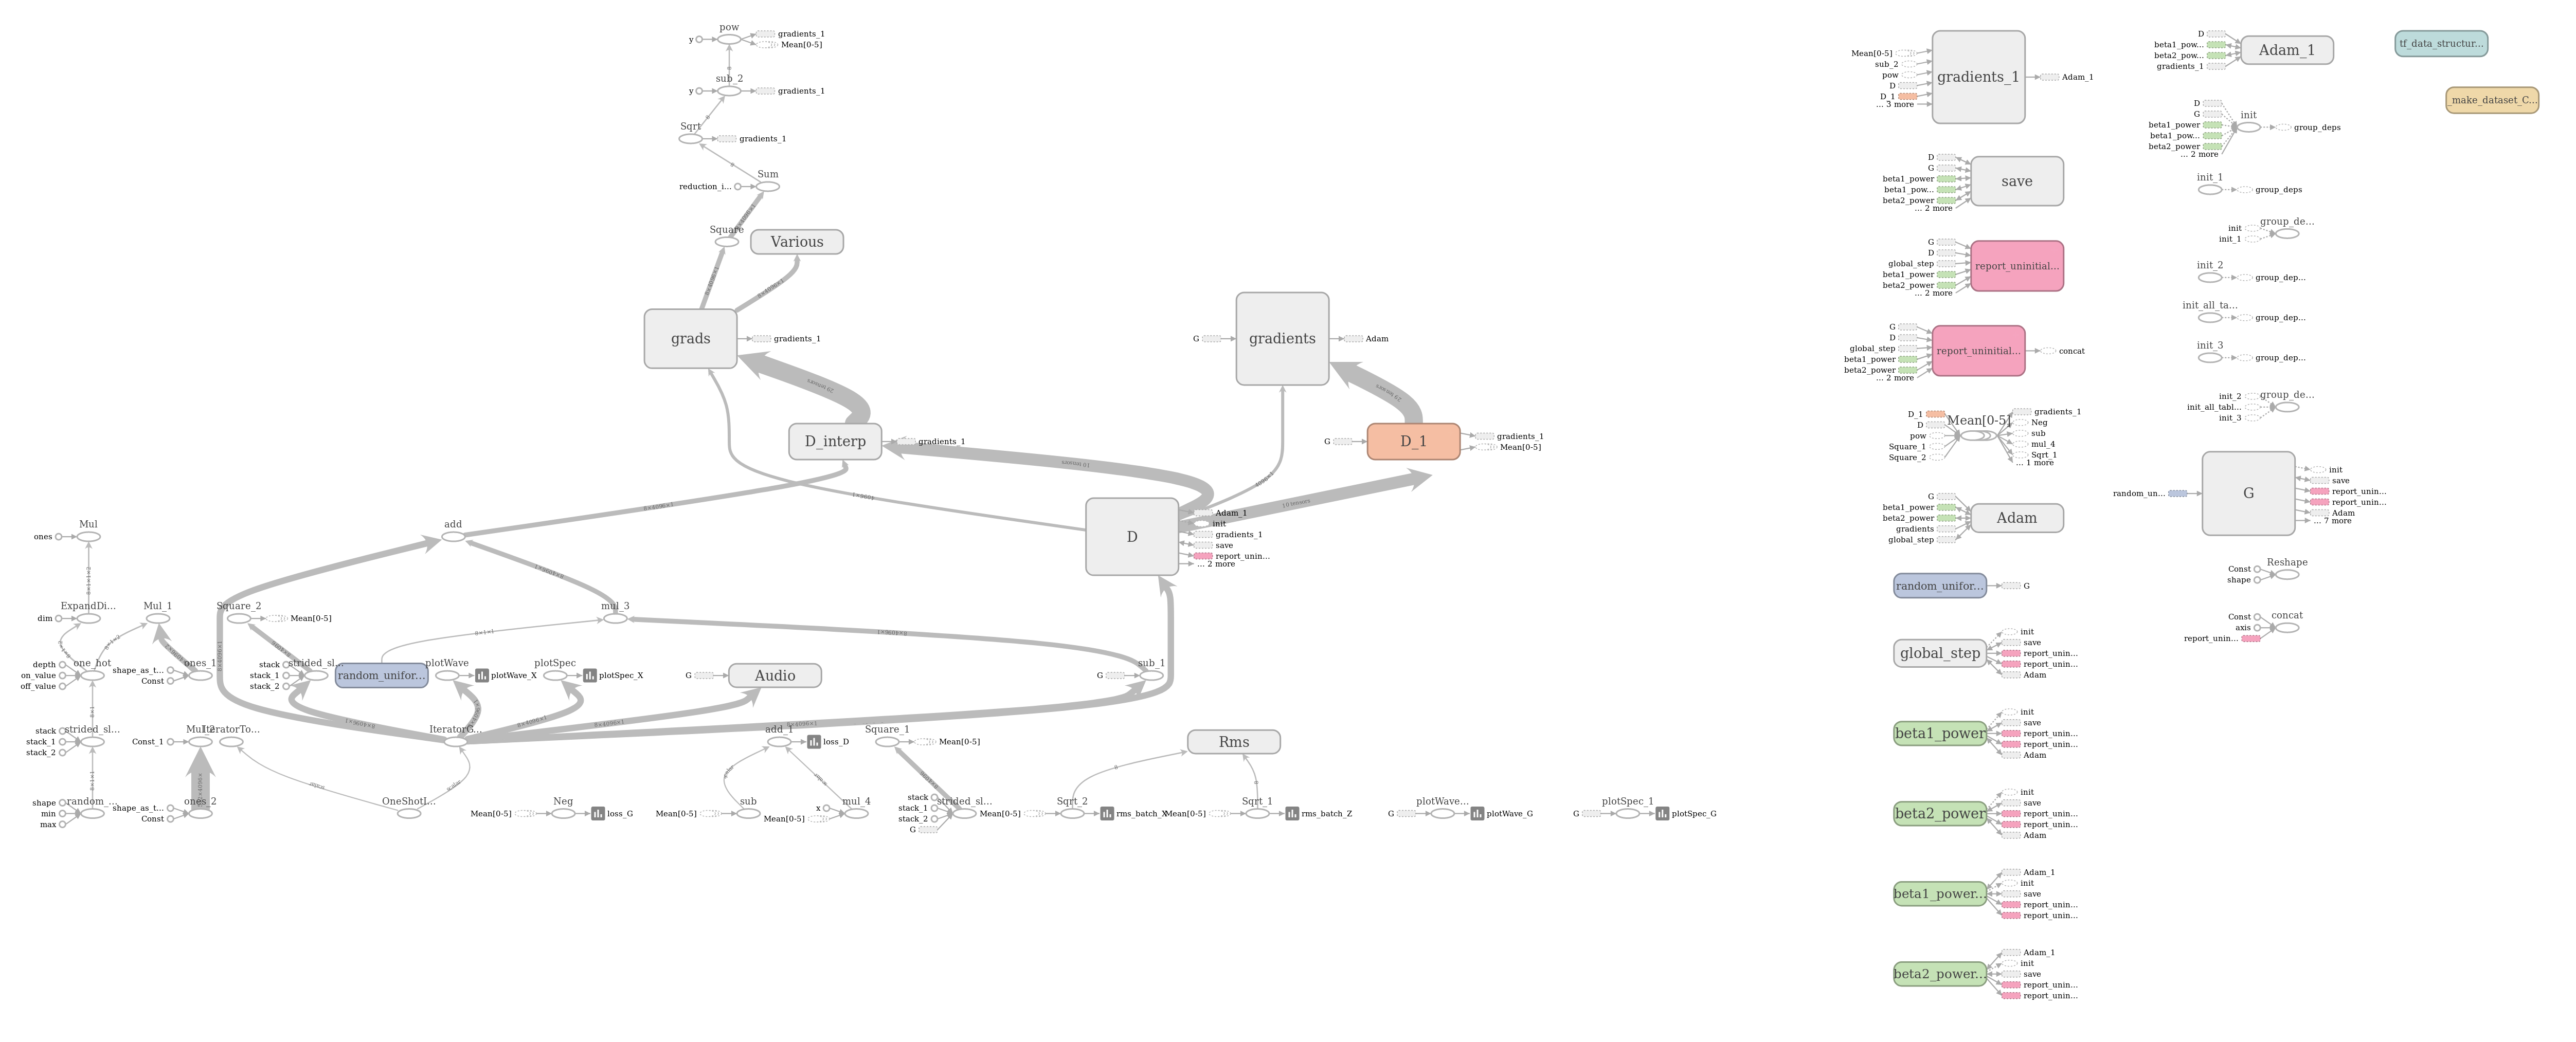
\includegraphics[width=1.25\textwidth, angle=90, trim={0 0 55cm 0}, clip]{WGAN}
  \end{figure}
  
  \clearpage

  \begin{figure}[ht]
    \caption{WaveGAN Model Auxiliary Nodes}
    \centering
    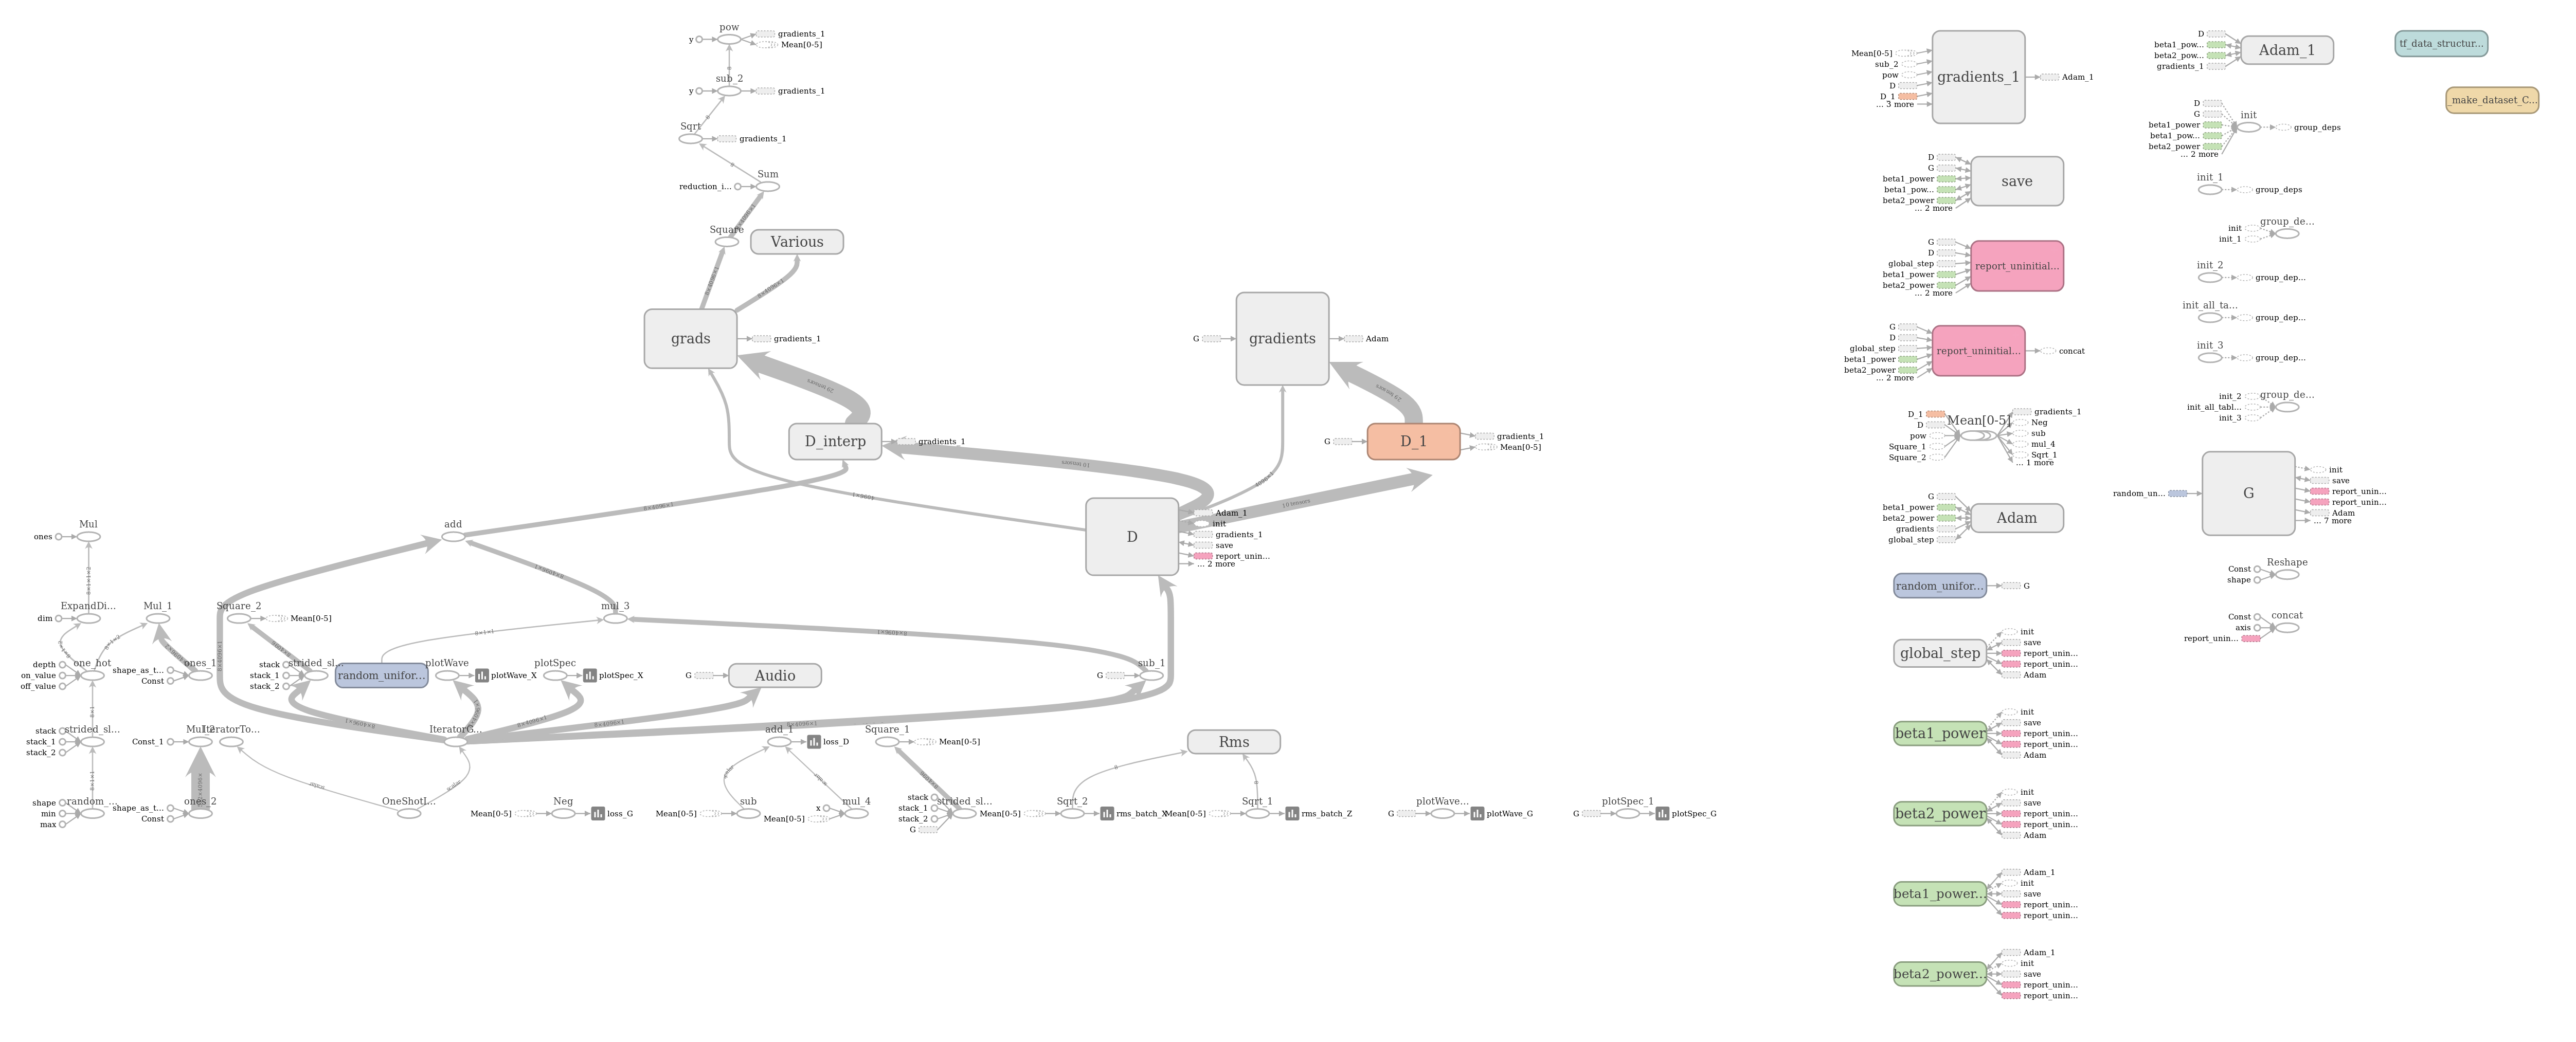
\includegraphics[width=1\textwidth, trim={120cm 0 0 0}, clip]{WGAN}
  \end{figure}
  \clearpage

  \begin{figure}[ht]
    \caption{Concatenated Conditional WaveGAN Model Main Graph}
    \centering
    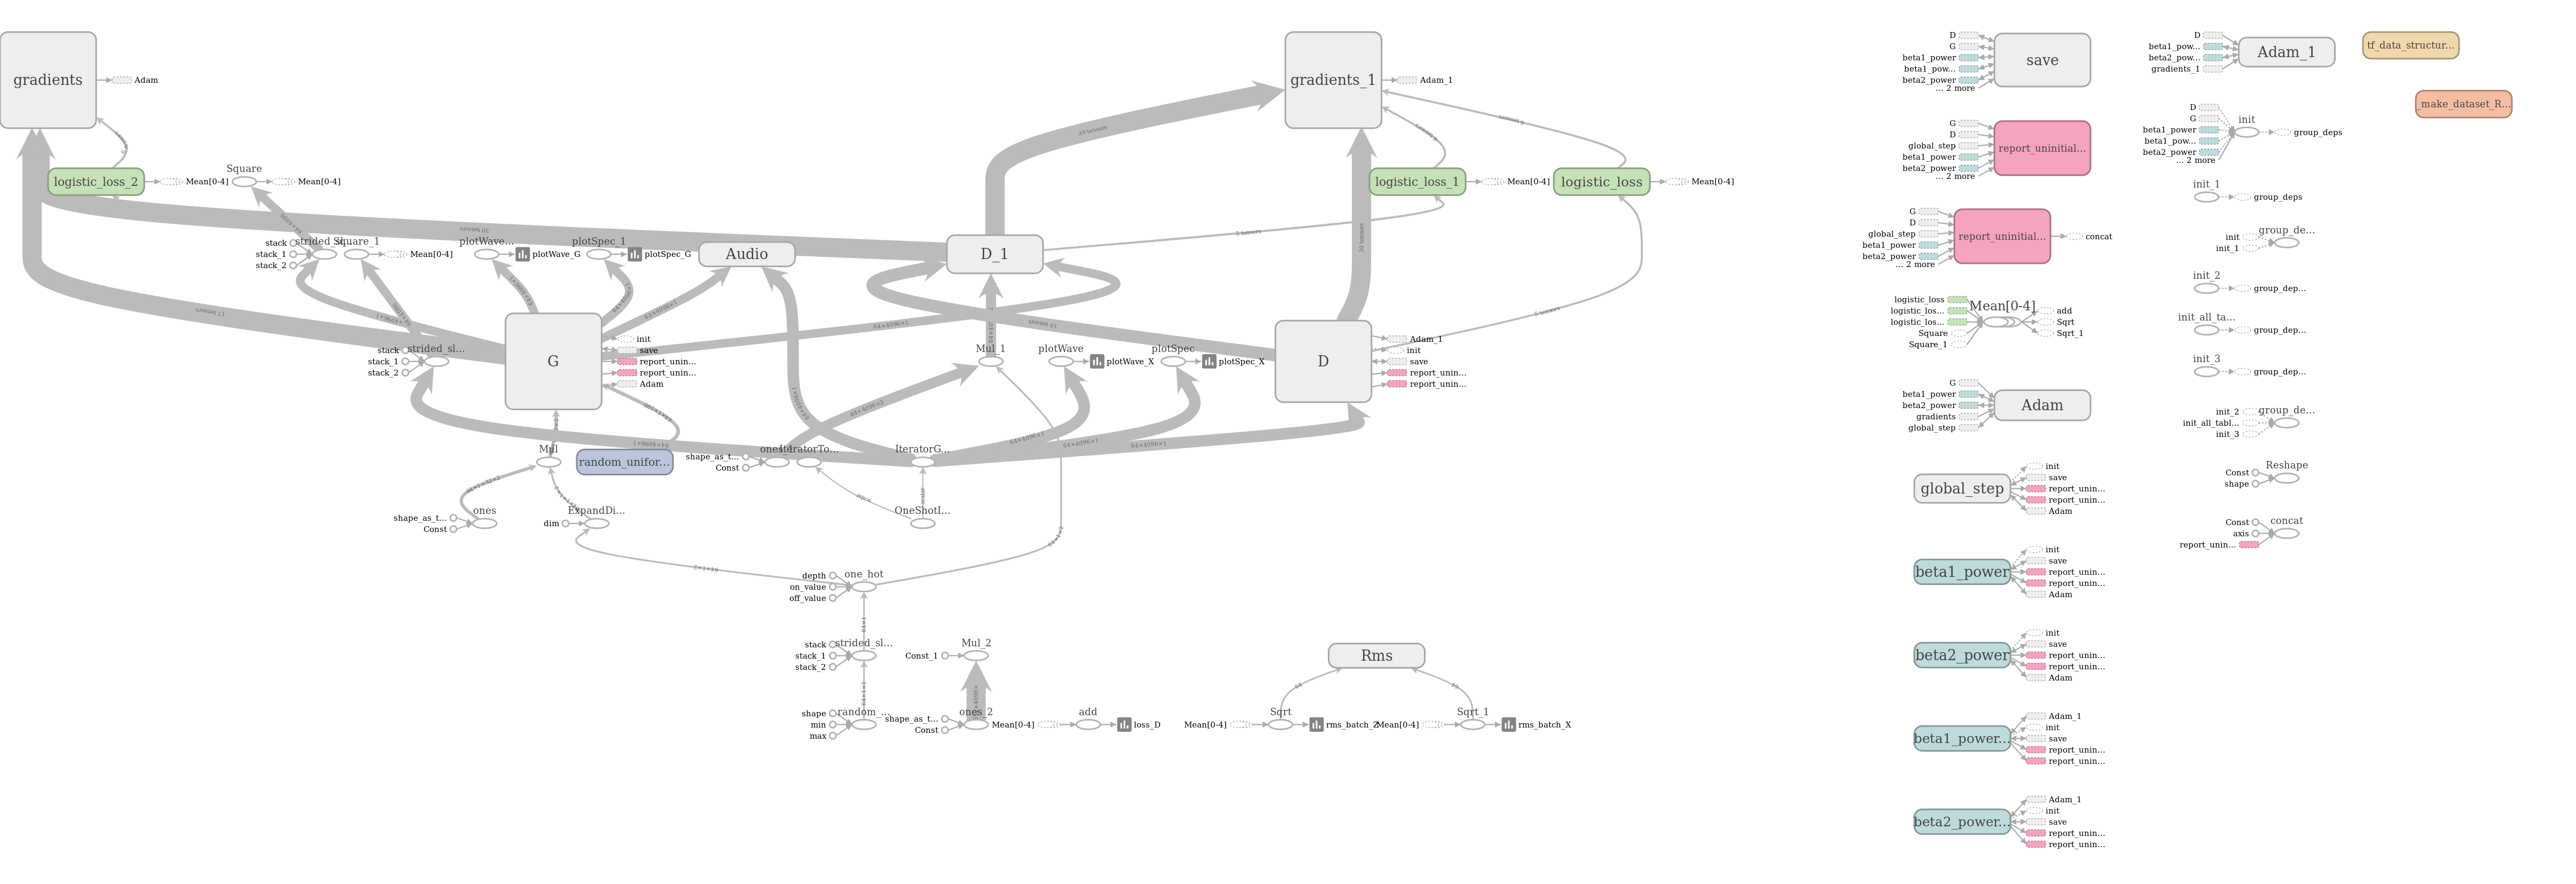
\includegraphics[width=1.25\textwidth, angle=90, trim={0 0 50cm 0}, clip]{cWGAN}
  \end{figure}
  
  \clearpage

  \begin{figure}[ht]
    \caption{Concatenated Conditional WaveGAN Model Auxiliary Nodes}
    \centering
    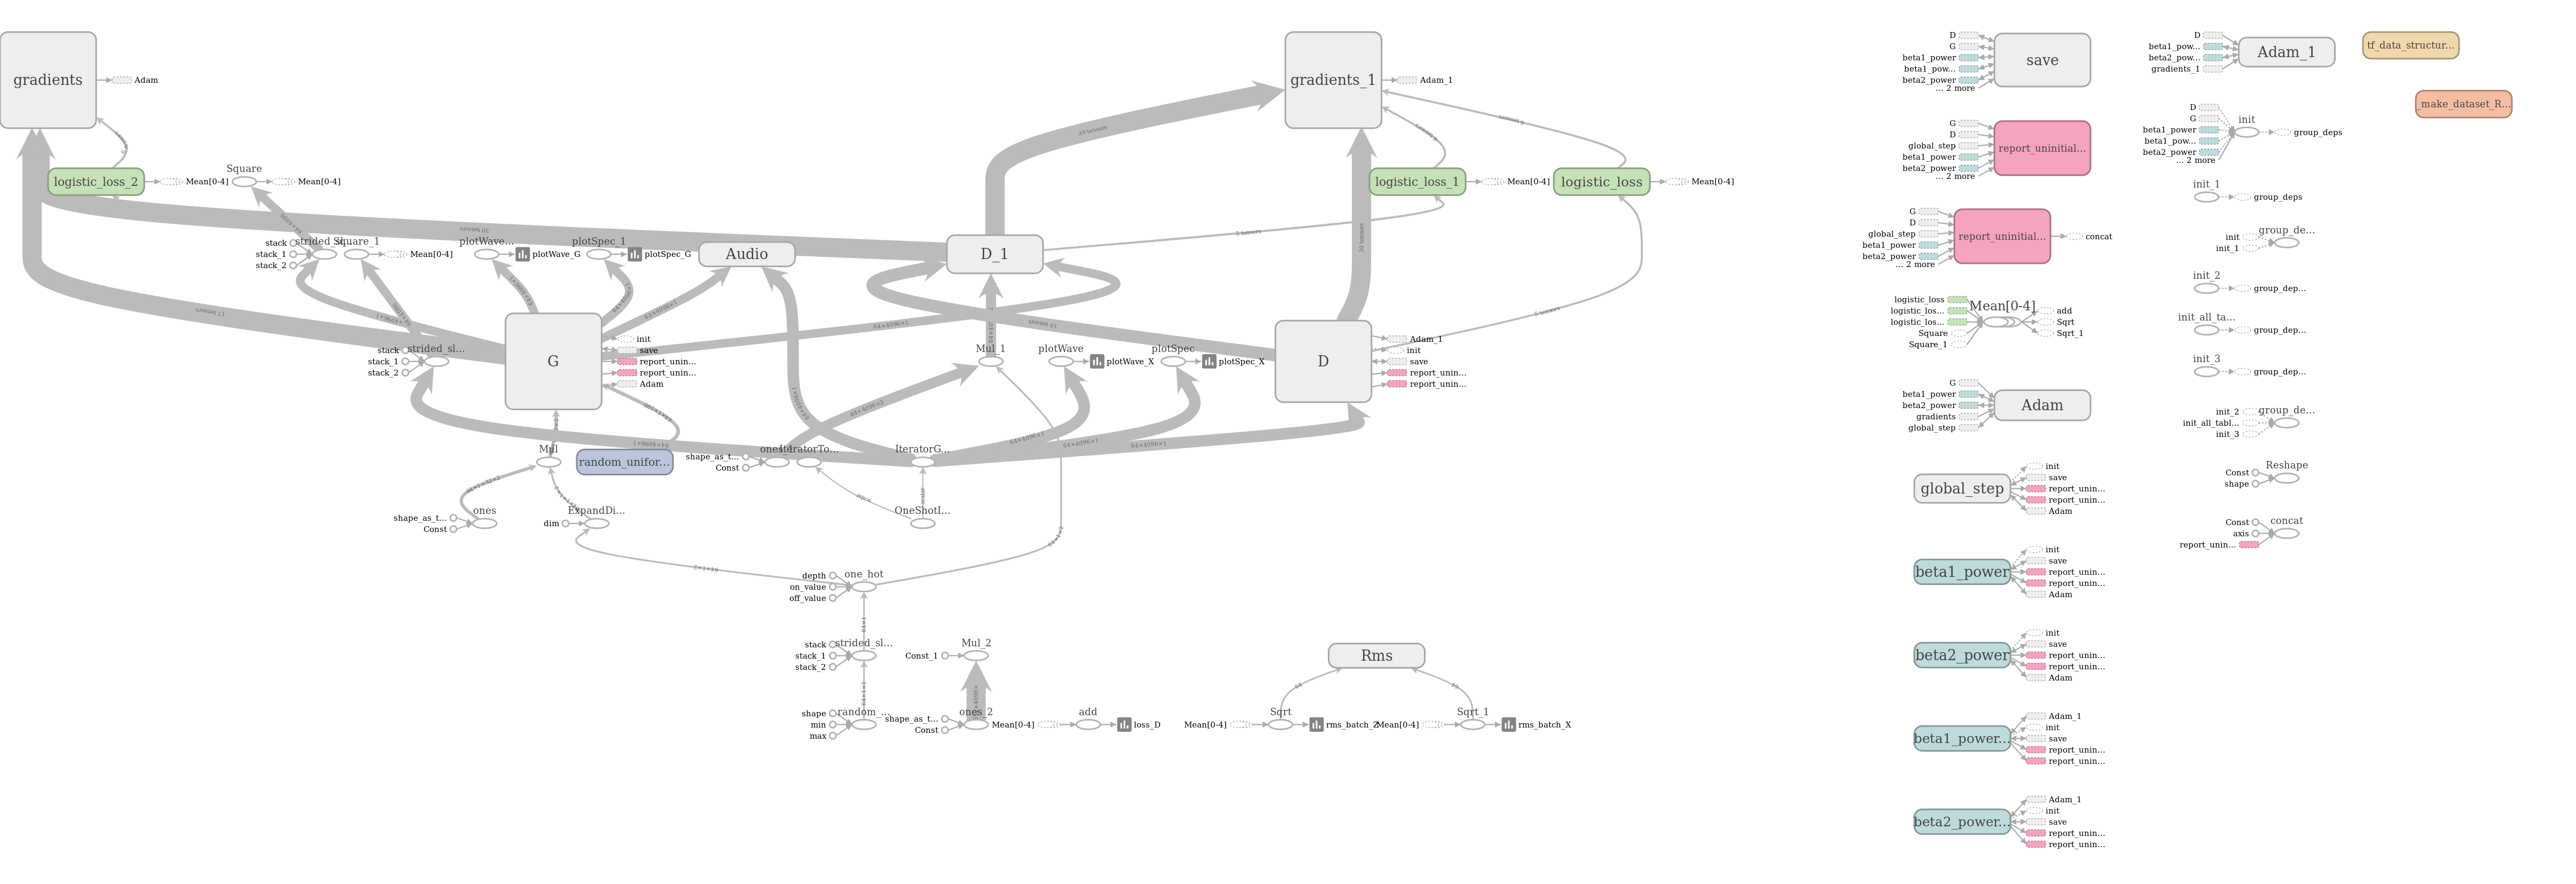
\includegraphics[width=1\textwidth, trim={120cm 0 0 0}, clip]{cWGAN}
  \end{figure}
  \clearpage

  \begin{figure}[ht]
    \caption{Auxiliary Classifier Conditional WaveGAN Model Main Graph}
    \centering
    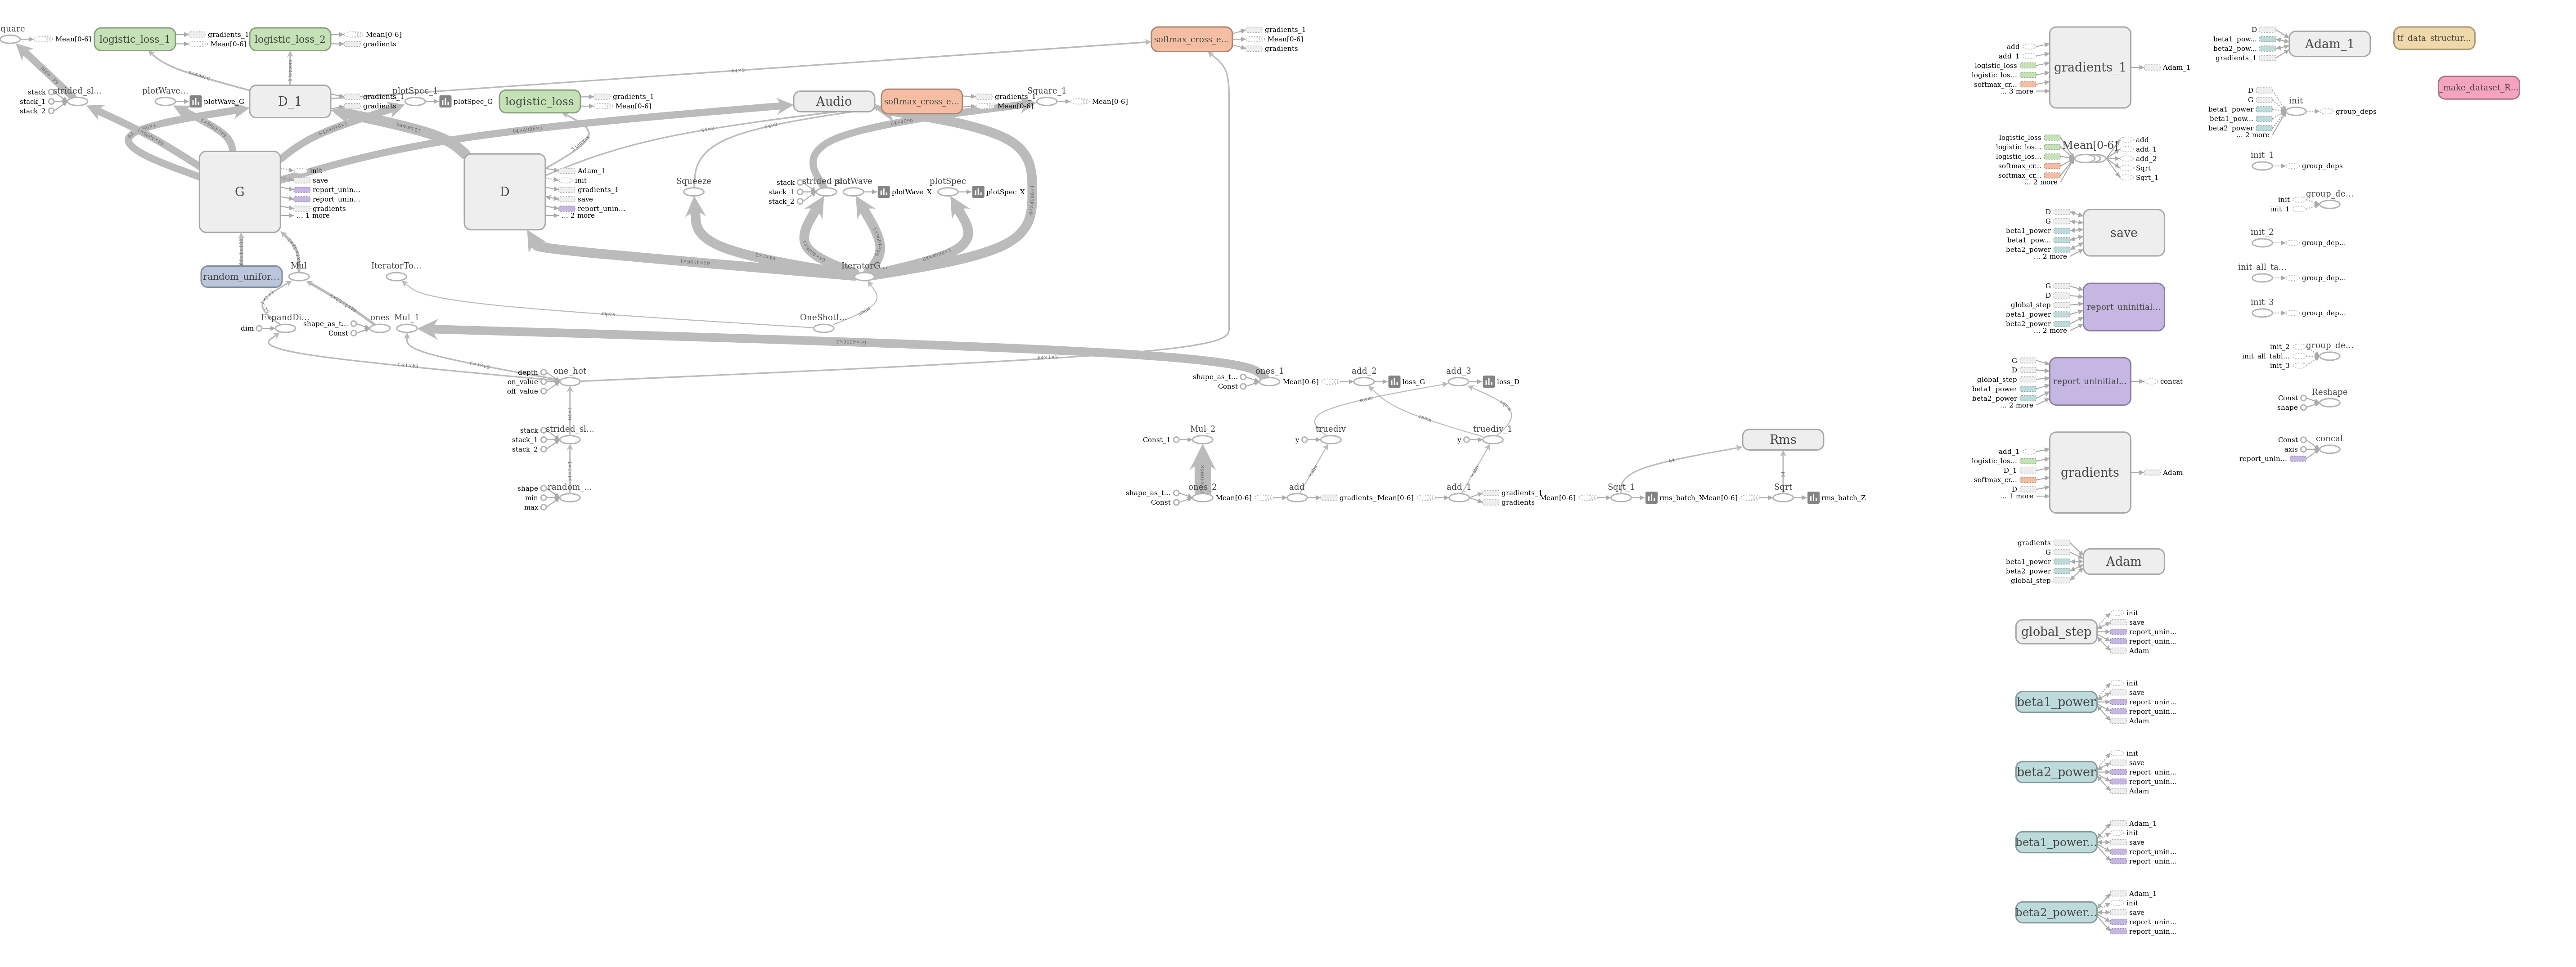
\includegraphics[width=1.25\textwidth, angle=90, trim={0 0 50cm 0}, clip]{ACGAN}
  \end{figure}
  
  \clearpage

  \begin{figure}[ht]
    \caption{Auxiliary Classifier Conditional WaveGAN Model Auxiliary Nodes}
    \centering
    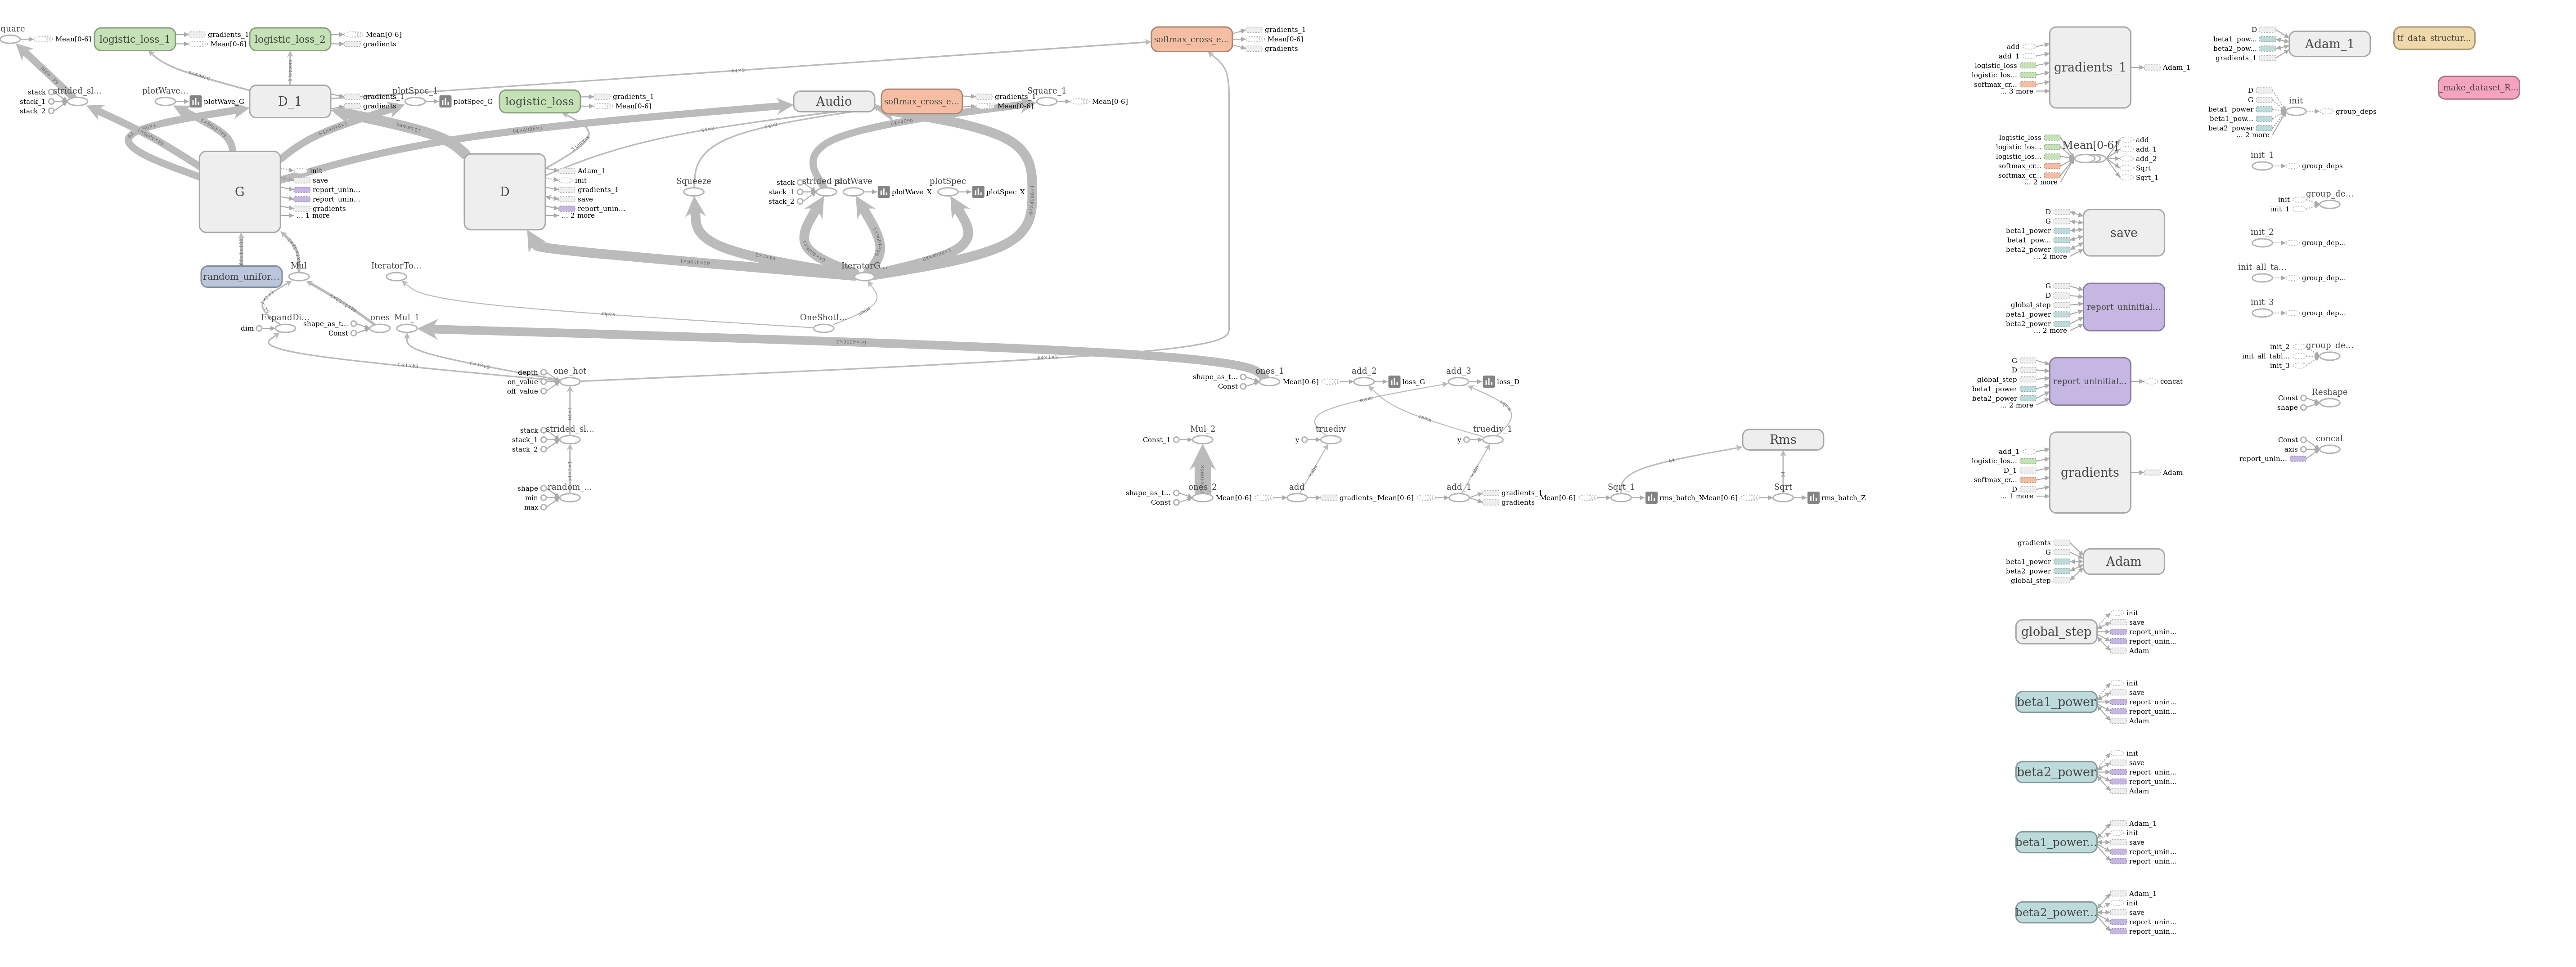
\includegraphics[width=1\textwidth, trim={150cm 0 0 0}, clip]{ACGAN}
  \end{figure}
  \clearpage
  
  \section{Hyperparameter Search Test Results}

  The following tables show the results of various tests that were used to reveal the potential best hyperparameters for the model.
  \newline
  \newline
  Test were initially run with two different conditional WaveGAN models but I've only included results from the better of the two as it consistently produced better results.
  The number of iterations are rounded down to the nearest thousand.
  
  \begin{table}[ht]
    
    \caption{Table of WaveGAN Learning Rate Experiments}
    \label{tab:WGAN_LR}
    
    \begin{center}
      \begin{tabular}{ r | r | r }
        
        Runs & 0.0001 & 0.00001 \\
        \hline
        1 & 2k & 5k \\
        2 & 5k & 5k \\
        3 & 4k & 5k \\
        4 & 4k & 5k \\
        5 & 4k & 5k \\
        6 & 3k & 5k \\
        7 & 3k & 5k \\
        8 & 5k & 5k \\
        9 & 4k & 5k \\
        10 & 3k & 5k \\
        \hline
        Avg. & 3.7k & 5k \\
        
      \end{tabular}
    \end{center}
    
  \end{table}

  \begin{table}[ht]
    
    \caption{Table of Conditional WaveGAN Learning Rate Experiments}
    \label{tab:CWGAN_LR}
    
    \begin{center}
      \begin{tabular}{ r | r | r }
        
        Runs & 0.0001 & 0.00001 \\
        \hline
        1 & 1k & 5k \\
        2 & 0 & 5k \\
        3 & 0 & 4k \\
        4 & 0 & 5k \\
        5 & 1k & 5k \\
        6 & 0 & 5k \\
        7 & 0 & 5k \\
        8 & 0 & 3k \\
        9 & 0 & 5k \\
        10 & 0 & 4k \\
        \hline
        Avg. & 0.2k & 4.5k \\
        
      \end{tabular}
    \end{center}
    
  \end{table}

  \begin{table}[ht]
    
    \caption{Table of WaveGAN Batch Size Experiments}
    \label{tab:WGAN_BS}
    
    \begin{center}
      \begin{tabular}{ r | r | r | r | r }
        
        Runs & 8 & 16 & 32 & 64 \\
        \hline
        1 & 5k & 5k & 3k & 3k \\
        2 & 5k & 5k & 5k & 4k \\
        3 & 4k & 4k & 4k & 3k \\
        4 & 5k & 4k & 4k & 3k \\
        5 & 5k & 5k & 5k & 3k \\
        6 & 4k & 5k & 5k & 3k \\
        7 & 4k & 3k & 5k & 5k \\
        8 & 5k & 5k & 5k & 3k \\
        9 & 5k & 5k & 4k & 4k \\
        10 & 5k & 3k & 5k & 5k \\
        \hline
        Avg. & 4.7k & 4.4k & 4.6k & 3.6k \\
        
      \end{tabular}
    \end{center}
    
  \end{table}

  \begin{table}[ht]
    
    \caption{Table of Conditional WaveGAN Batch Size Experiments}
    \label{tab:CWGAN_BS}
    
    \begin{center}
      \begin{tabular}{ r | r | r | r | r }
        
        Runs & 8 & 16 & 32 & 64 \\
        \hline
        1 & 2k & 0 & 1k & 0 \\
        2 & 0 & 0 & 0 & 0 \\
        3 & 0 & 0 & 0 & 0 \\
        4 & 0 & 0 & 0 & 2k \\
        5 & 0 & 0 & 0 & 1k \\
        6 & 0 & 0 & 3k & 0 \\
        7 & 0 & 0 & 0 & 0 \\
        8 & 0 & 5k & 0 & 1k \\
        9 & 0 & 0 & 0 & 0 \\
        10 & 1k & 0 & 0 & 0k \\
        \hline
        Avg. & 0.3k & 0.5k & 0.4k & 0.4k \\
        
      \end{tabular}
    \end{center}
    
  \end{table}

  \begin{table}[ht]
    
    \caption{Table of WaveGAN Lambda Experiments}
    \label{tab:WGAN_LAM}
    
    \begin{center}
      \begin{tabular}{ r | r | r | r | r }
        
        Runs & 10 & 100 \\
        \hline
        1 & 3k & 5k \\
        2 & 3k & 4k \\
        3 & 5k & 3k \\
        4 & 4k & 5k \\
        5 & 4k & 5k \\
        6 & 3k & 5k \\
        7 & 5k & 5k \\
        8 & 3k & 5k \\
        9 & 4k & 5k \\
        10 & 4k & 5k \\
        \hline
        Avg. & 3.7k & 4.5k \\
        
      \end{tabular}
    \end{center}
    
  \end{table}

  \begin{table}[ht]
    
    \caption{Table of Conditional WaveGAN Lambda Experiments}
    \label{tab:CWGAN_LAM}
    
    \begin{center}
      \begin{tabular}{ r | r | r | r | r }
        
        Runs & 10 & 100 \\
        \hline
        1 & 0 & 0 \\
        2 & 0 & 1k \\
        3 & 0 & 1k \\
        4 & 0 & 1k \\
        5 & 0 & 3k \\
        6 & 0 & 0 \\
        7 & 0 & 0 \\
        8 & 0 & 1k \\
        9 & 0 & 3k \\
        10 & 0 & 0 \\
        \hline
        Avg. & 0 & 1k \\
        
      \end{tabular}
    \end{center}
    
  \end{table}

  \begin{table}[ht]

  \caption{Table of WaveGAN Number of Discriminator Updates Experiments}
    \label{tab:WGAN_Ds}
    
    \begin{center}
      \begin{tabular}{ r | r | r | r | r | r }
        
        Runs & 1 & 2 & 3 & 4 & 5 \\
        \hline
        1 & 3k & 1k & 5k & 5k & 0 \\
        2 & 5k & 1k & 0 & 5k & 0 \\
        3 & 3k & 1k & 1k & 0 & 0 \\
        4 & 5k & 5k & 0 & 0 & 0 \\
        5 & 5k & 1k & 0 & 0 & 0 \\
        6 & 3k & 2k & 1k & 0 & 0 \\
        7 & 4k & 1k & 1k & 0 & 0 \\
        8 & 5k & 5k & 0 & 1k & 0 \\
        9 & 4k & 1k & 5k & 0 & 0 \\
        10 & 3k & 1k & 0 & 0 & 0 \\
        \hline
        Avg. & 4k & 1.9k & 1.3k & 1.1k & 0 \\
        
      \end{tabular}
    \end{center}
    
  \end{table}

  \begin{table}[ht]

  \caption{Table of Conditional WaveGAN Number of Discriminator Updates Experiments}
    \label{tab:CWGAN_Ds}
    
    \begin{center}
      \begin{tabular}{ r | r | r | r | r | r }
        
        Runs & 1 & 2 & 3 & 4 & 5 \\
        \hline
        1 & 0 & 0 & 0 & 0 & 0 \\
        2 & 0 & 0 & 0 & 0 & 0 \\
        3 & 0 & 2k & 0 & 0 & 0 \\
        4 & 0 & 0 & 0 & 0 & 0 \\
        5 & 2k & 0 & 0 & 0 & 0 \\
        6 & 0 & 0 & 0 & 0 & 0 \\
        7 & 0 & 0 & 0 & 0 & 0 \\
        8 & 0 & 0 & 0 & 0 & 0 \\
        9 & 0 & 0 & 0 & 0 & 0 \\
        10 & 1k & 0 & 0 & 0 & 0 \\
        \hline
        Avg. & 0.3k & 0.2k & 0 & 0 & 0 \\
        
      \end{tabular}
    \end{center}
    
  \end{table}

  \clearpage

  \section{Code}

  The following pages include the code for the GAN high-level architecture and training functions (Manager.py), code for the neural networks (Networks-WGAN-4096.py, Networks-CWGAN-4096.py, and Networks-ACGAN-4096.py), and other code that was necessary to complete the project (audioDataLoader.py and Downsampler.py). 

  \subsection{Manager.py}

  \lstinputlisting[language=Python]{\CodePath/Experiment/Manager.py}

  \newpage

  \subsection{Networks-WGAN-4096.py}

  \lstinputlisting[language=Python]{\CodePath/Experiment/Networks-WGAN-4096.py}

  \newpage

  \subsection{Networks-CWGAN-4096.py}

  \lstinputlisting[language=Python]{\CodePath/Experiment/Networks-CWGAN-4096.py}

  \newpage

  \subsection{Networks-ACGAN-4096.py}

  \lstinputlisting[language=Python]{\CodePath/Experiment/Networks-CWGAN-4096.py}

  \newpage

  \subsection{audioDataLoader.py}

  \lstinputlisting[language=Python]{\CodePath/Experiment/audioDataLoader.py}

  \newpage

  \subsection{Downsampler.py}

  \lstinputlisting[language=Python]{\CodePath/Audio_Manipulation/Downsampler.py}

\end{appendices}

% Wrapup
\end{document}